\documentclass[12pt,onecolumn,titlepage]{article}
\usepackage{geometry} % see geometry.pdf on how to lay out the page. There's lots.
\geometry{letterpaper} % or letter or a5paper or ... etc
% \geometry{landscape} % rotated page geometry
\usepackage{hyperref}
\usepackage{graphicx}


%For subfigures/subfloats
%\usepackage[caption=false,font=footnotesize]{subfig}
%\usepackage{caption}
%\usepackage{subcaption}
\usepackage{subfigure}

%For including eps graphics, as well as updating the figures upon recompiling
\usepackage[update,prepend]{epstopdf}

%AMS math package
\usepackage{amsmath}

%For emoticons :)
\usepackage{wasysym}



\title{Daily Log}
\author{Jordan Seth Besnoff \\ Duke University \\ ECE Department \\ \href{mailto:jordan.besnoff@duke.edu}{\nolinkurl{jordan.besnoff@duke.edu}}}
\date{26 March 2012} % delete this line to display the current date

%%% BEGIN DOCUMENT
\begin{document}

\maketitle
\tableofcontents

\newpage

\section{26 March 2012:}

\textbf{Time in: 9:00 AM} \\
\textbf{Time out: 6:15 PM} \\

Much of today's work focused on matching a small loop antenna to the NXP tag chips, the SL3S1002FTB1 chip with the TSSOP8 package (the larger chip with 8 pins). Matching with this chip had been attempted before, but without much success. Problems with earlier matching attempts may be due to a few factors: the calibration plane (when using the network analyzer), mode of calibration, power level from the network analyzer, and the reported impedance value from NXP. 

Impedance values read off the network analyzer for the NXP chip were drastically different from that reported in the data sheet, as shown below. This caused the first round of matching to be quite inaccurate, as matching was performed to the specifications as noted on the data sheet, which is seemingly not an accurate representation of the impedance. 

In order to check if the calibration of the network analyzer was done correctly, a single inductor of a known value (plus or minus 5\%) was connected to a coaxial connector, and then to the network analyzer to see if the correct inductance could be read off the smith chart ($R+jX$). Once the inductance was properly verified, the small loop (9.50 mm diameter) and chip were tested. As a secondary check, the electrical delay of the network analyzer was altered so that the open condition was properly set. The electrical delay altered case was not explored while performing matching. Matching was then performed with the chip to match it to $50 \Omega$. After talking with Daniel about calibration planes and the data from the NXP spec sheet, a new calibration was performed with custom made short and load connectors, hopefully shifting the calibration plane to where the chip is seated. The power levels were also altered as the chip is a non-linear device and so is frequency dependent, and because of the existence of a power harvester on the chip. This will cause the components on the chip to function for certain power levels above a threshold (about -15 dBm according to the spec sheet), and below this point, the power drawn will drop. This is essential to reported impedance values on the spec sheet.

\subsection{Inductor Impedance Tests}
\indent \indent Calibration was performed using the short, open and load coaxial connectors in the SMA box near the network analyzer, not the calibration kit. Span was set from 800 MHz to 1 GHz, and the power level was set to the default value of 0 dBm. Measurements were performed with and without an electrical delay of 63.1 psec, as this value placed the open condition at the right end of the real line on the smith chart where it belongs for a true open. The results of this test are shown below in Figures \ref{fig:inductor_100nH} and \ref{fig:inductor_100nH_elec_delay}.

\begin{figure}[h!]
	\centering
	\subfigure[100 nH Inductor, no electrical delay]{
	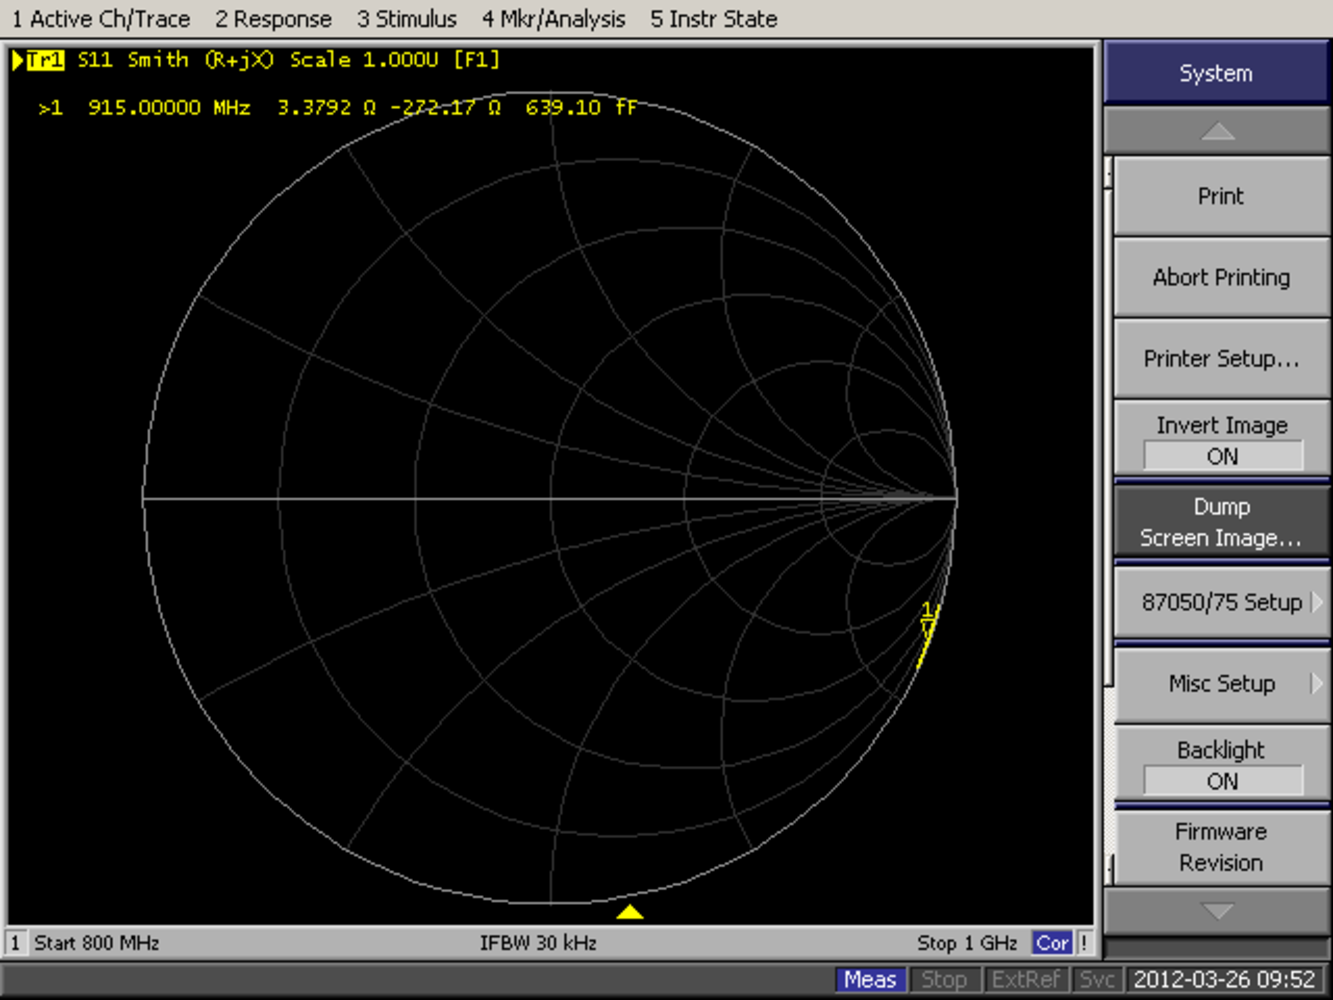
\includegraphics[width=2.8in]{Pictures/26Mar2012/INDUCTOR_100NH} 
	\label{fig:inductor_100nH}
	}
	\subfigure[100 nH Inductor, with 63.1 psec electrical delay]{
	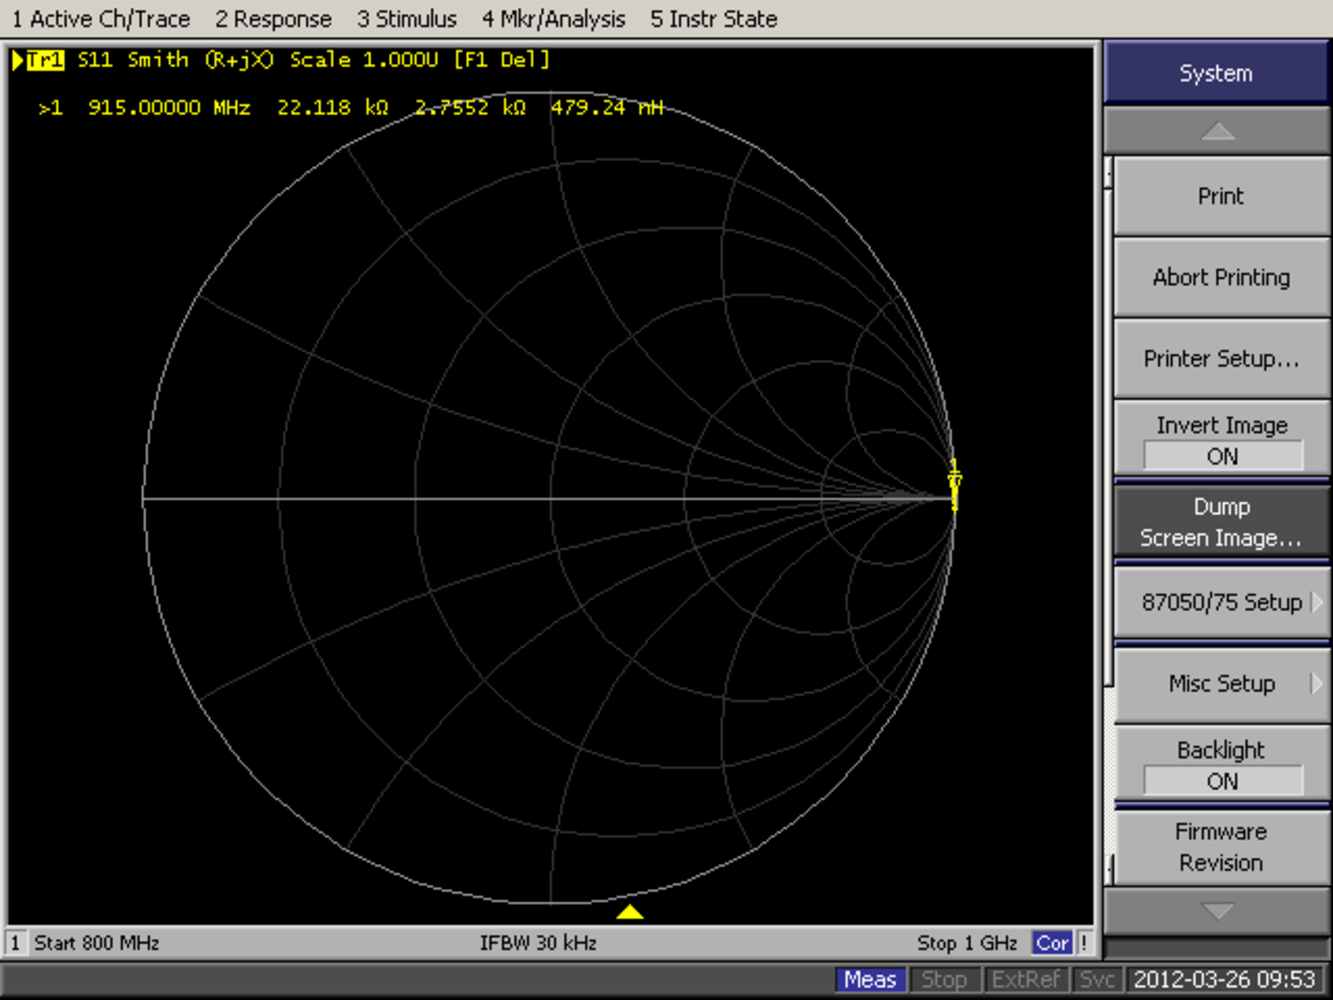
\includegraphics[width=2.8in]{Pictures/26Mar2012/INDUCTOR_100NH_ELEC_DELAY} 
	\label{fig:inductor_100nH_elec_delay}
	}
	\label{fig:inductor_test1}
	\caption{Singular Inductor Connected To Straight Coaxial Connector}
%	\caption[Optional caption for list of figures]{Backscattered signal strength as a function of
%	distance in the saline proxy for various carrier frequencies. Modulated backscatter of 
%	7.5 MHz in \subref{fig:backscatter_f75}, 15MHz in \subref{fig:backscatter_f15}, and 
%	30 MHz in \subref{fig:backscatter_f30}.}
\end{figure}

In the measurement with no electrical delay, the inductor appears capacitive, with a capacitance of $639.10$ fF. When the electrical delay was used to correct for open condition, the inductor appears inductive with an inductance of $479.24$ nH. All these values are taken at the frequency of interest of 915 MHz. This large error in both cases may be due to the fact that we're on the outer edge of the smith chart, where the network analyzer's error is larger. Another source of error may be the calibration plane, as the inductor is located at the edge of the coaxial pins, and the short used for calibration is close to the mating plane of the connector. Those few mm can make a large difference since the frequency of interest is 915 MHz. 

\subsection{Loop Impedance Tests}
\indent \indent The small loop antenna, diameter of 9.50 mm, was tested in a similar manner to the inductor, using the same settings. The results from testing the impedance of the small loop at 915 MHz are shown below in Figures \ref{fig:loop} and \ref{fig:loop_elec_delay}.

\begin{figure}[h!]
	\centering
	\subfigure[9.50 mm loop, no electrical delay]{
	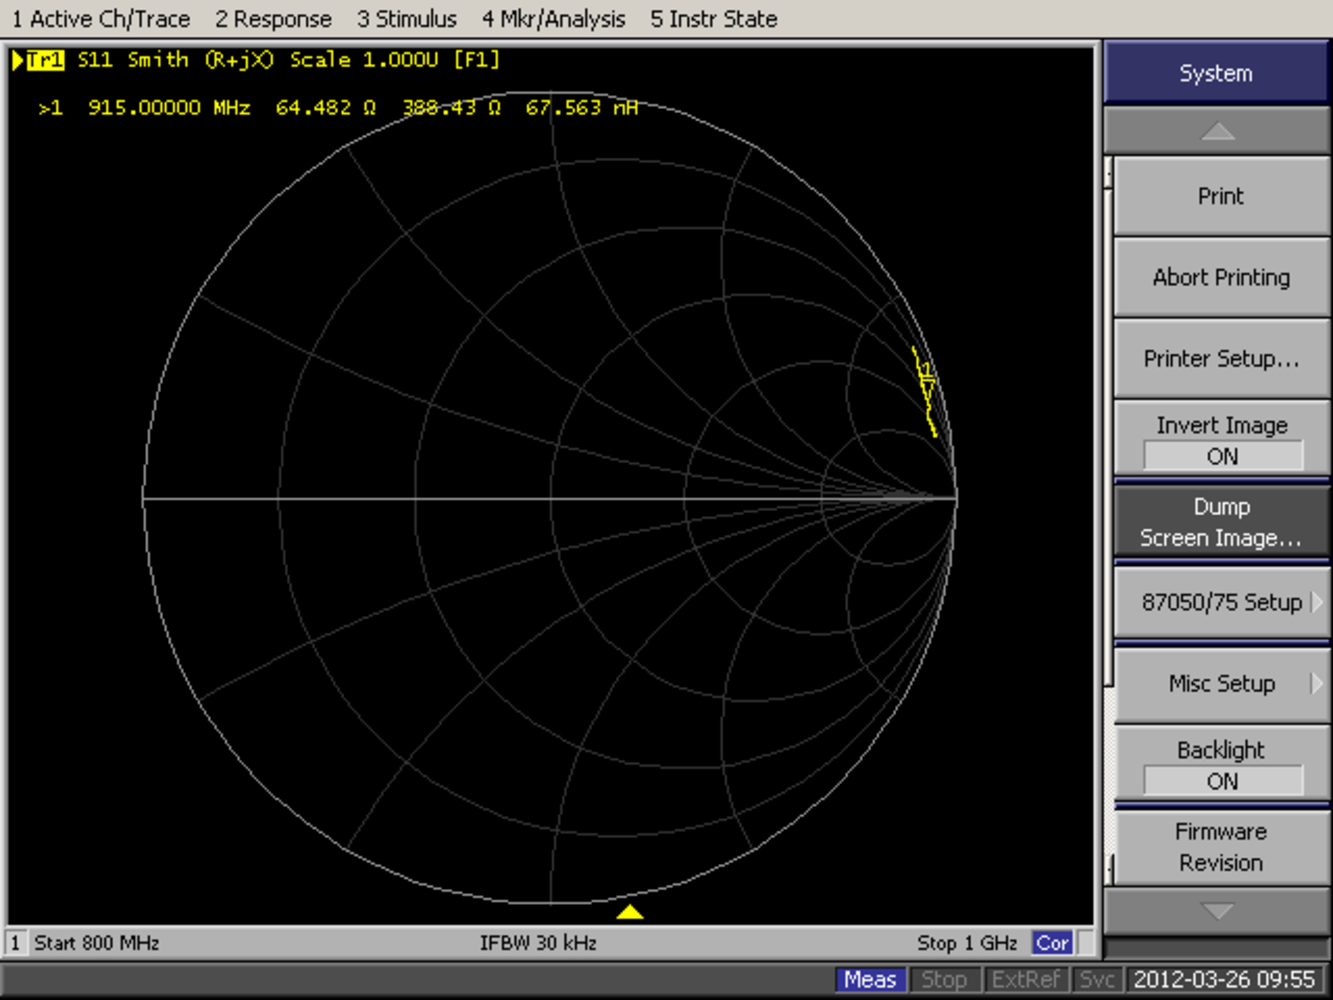
\includegraphics[width=2.8in]{Pictures/26Mar2012/LOOP} 
	\label{fig:loop}
	}
	\subfigure[9.50 mm loop, with 63.1 psec electrical delay]{
	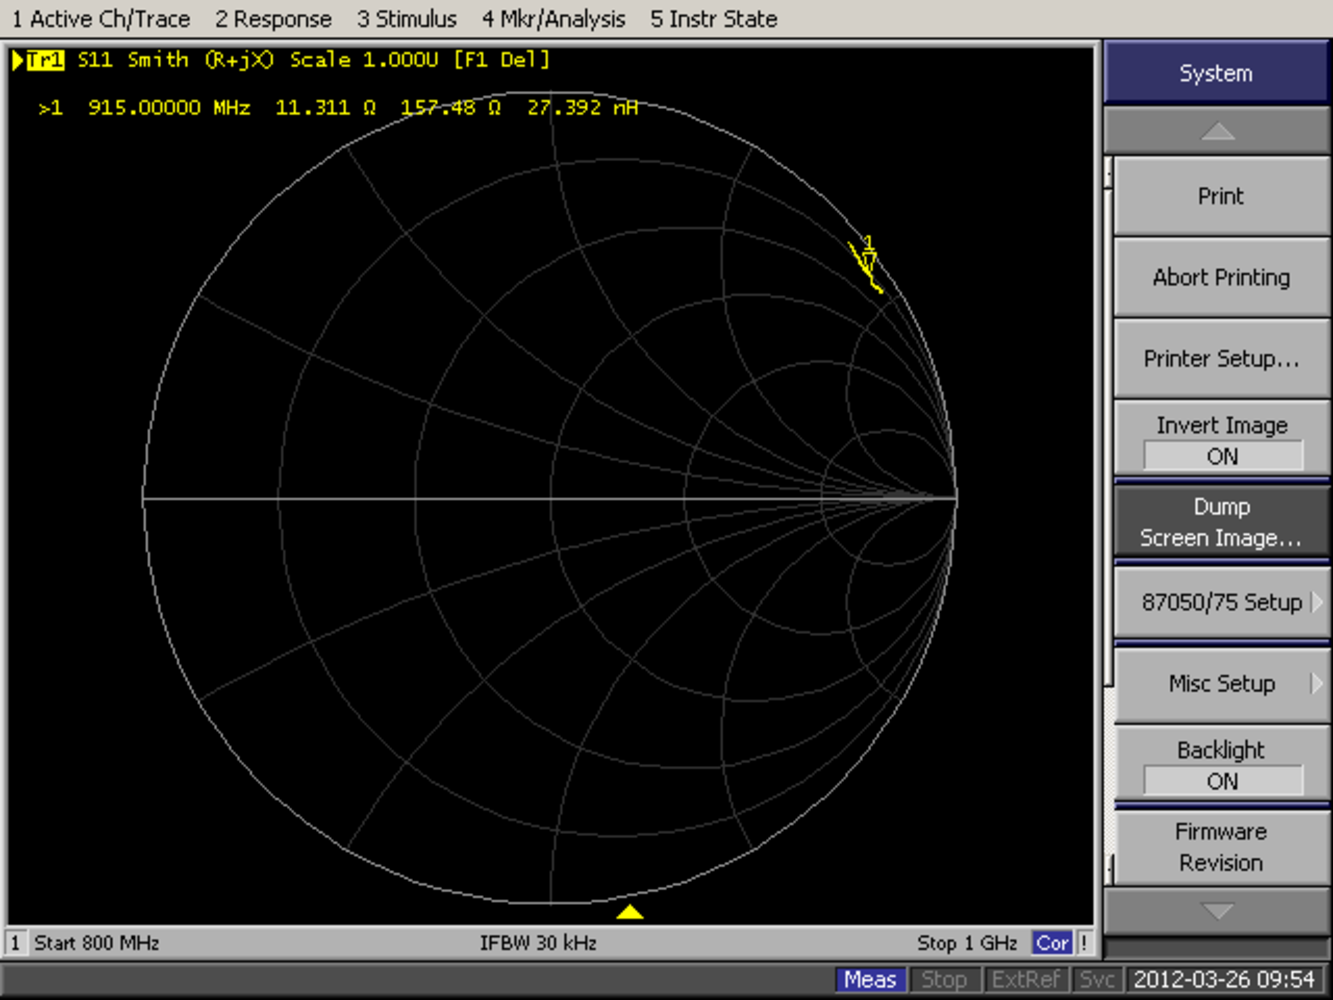
\includegraphics[width=2.8in]{Pictures/26Mar2012/LOOP_ELEC_DELAY} 
	\label{fig:loop_elec_delay}
	}
	\label{fig:loop_test1}
	\caption{Impedance Of Small Loop Antenna, Diameter = 9.50 mm}
%	\caption[Optional caption for list of figures]{Backscattered signal strength as a function of
%	distance in the saline proxy for various carrier frequencies. Modulated backscatter of 
%	7.5 MHz in \subref{fig:backscatter_f75}, 15MHz in \subref{fig:backscatter_f15}, and 
%	30 MHz in \subref{fig:backscatter_f30}.}
\end{figure}

As expected, the loop appears inductive, both with and without a corrective electrical delay. Unfortunately, it appears that the measured values for the loop don't match up with simulations obtained from Agilent ADS and CST Microwave Studio (not shown here, will include in the future...). Without the electrical delay, the loop's impedance is about $Z=64.5+j388.4\Omega$, which corresponds to an inductance of 67.6 nH, and with the electrical delay the impedance is $Z=11.3+j157.5\Omega$, for an inductance of 27.4 nH.

\subsection{Chip Impedance Tests}
\indent \indent The chip impedance was again tested in the same manner as the inductor and the small loop antenna. Note here the power level is 0 dBm. The impedance measurements are shown below in Figures \ref{fig:chip} and \ref{fig:chip_elec_delay}.

\begin{figure}[ht!]
	\centering
	\subfigure[Chip impedance, no electrical delay]{
	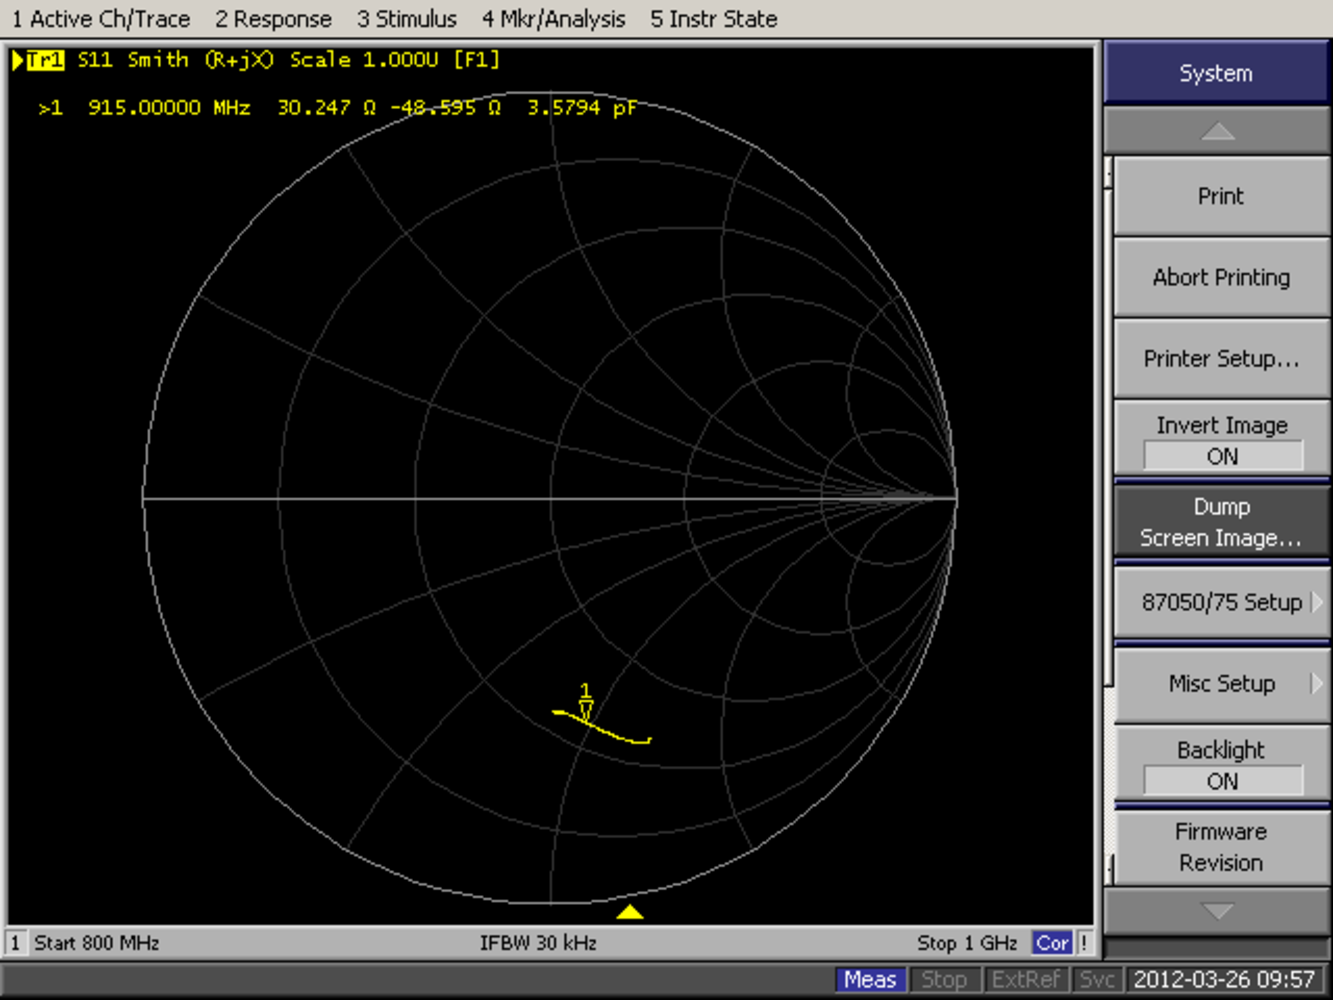
\includegraphics[width=2.8in]{Pictures/26Mar2012/CHIP} 
	\label{fig:chip}
	}
	\subfigure[Chip impedance, with 63.1 psec electrical delay]{
	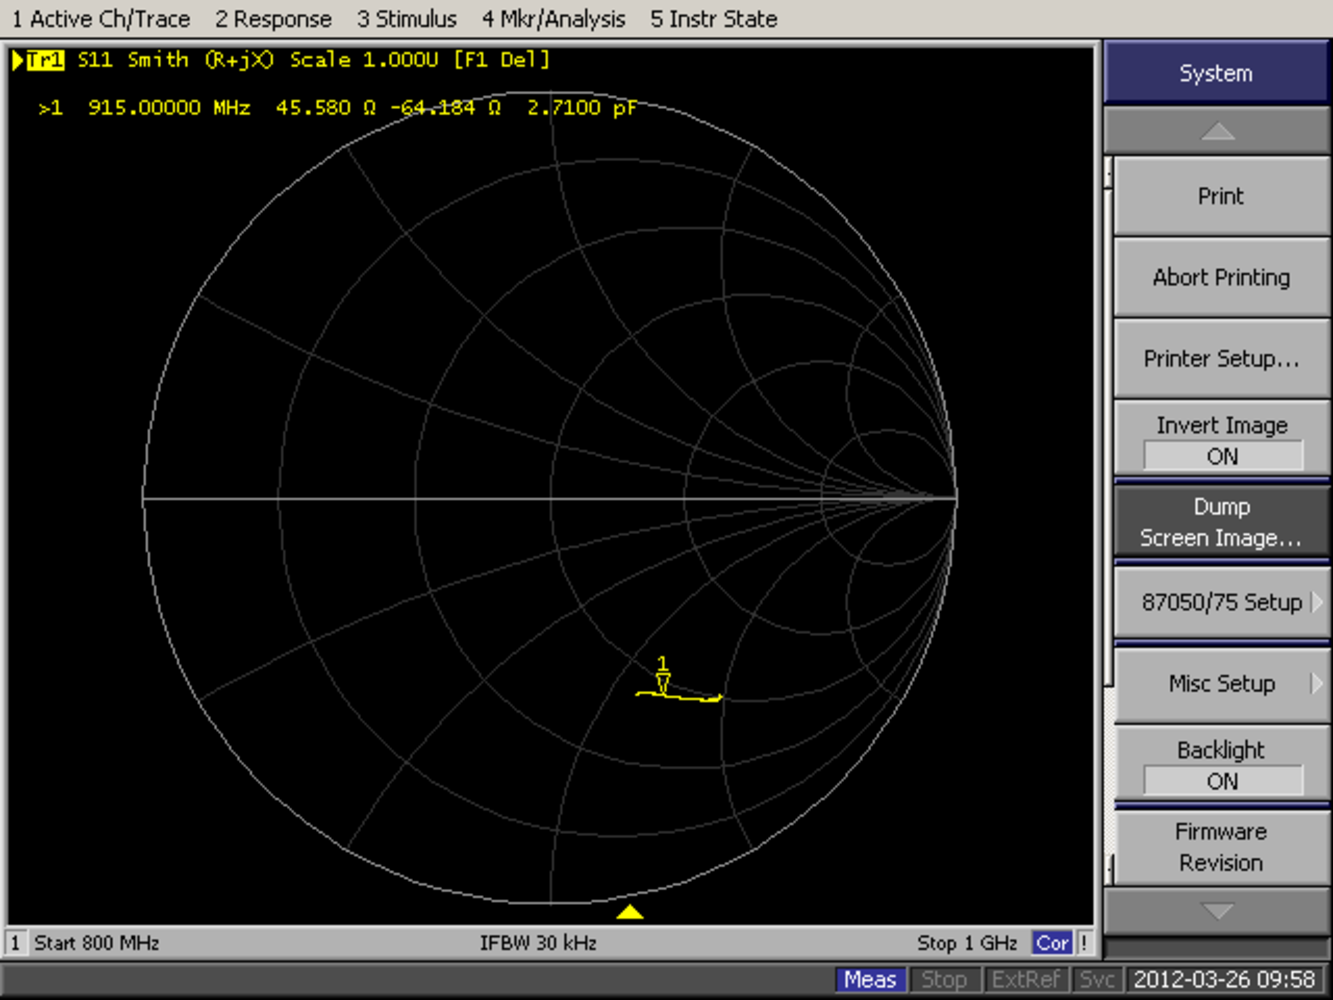
\includegraphics[width=2.8in]{Pictures/26Mar2012/CHIP_ELEC_DELAY} 
	\label{fig:chip_elec_delay}
	}
	\label{fig:loop_test1}
	\caption{Impedance Of NXP SL3S1002FTB1 chip with the TSSOP8 package}
%	\caption[Optional caption for list of figures]{Backscattered signal strength as a function of
%	distance in the saline proxy for various carrier frequencies. Modulated backscatter of 
%	7.5 MHz in \subref{fig:backscatter_f75}, 15MHz in \subref{fig:backscatter_f15}, and 
%	30 MHz in \subref{fig:backscatter_f30}.}
\end{figure}

Without the electrical delay, $Z=29.7-j45.9\Omega$, which is about 3.39 pF, and with the electrical delay $Z=45.6-j64.2\Omega$, or 2.71 pF. These values are significantly different from the reported value on the spec sheet for this package of $Z=16-j148\Omega$, which is 

%Future stuff:
%Inductor: smaller value, closer to 5 nH or so, to get a better reading, and do this with the new calibration setup



%31 May 2012
\clearpage
\section{31 May 2012:}

%\textbf{Time in: 9:45 AM} \\
%\textbf{Time out:  PM} \\


\indent \indent Focusing on matching both the NXP tag chip (SL3S1002FTB1 chip with the TSSOP8 package) and the small loop antenna (9.50 mm diameter) to 50 $\Omega$ in the saline tank. The calibration here was performed using the Agilent calibration kit (85033E) outside of the tank. Since the calibration kit is sealed, the calibration should not change once inside the tank. No manual calibration correction was performed here (ie: using the electrical delay to move the short \& open to the correct spots on the smith chart), since as long as both the loop and chip are matched to the same relative point with the same calibration, they will be matched when combined. 

\subsection{NXP Tag Chip Impedance in Saline Using Agilent Cal}
\indent \indent The impedance of the NXP tag chip using the calibration described above is shown below in Figure \ref{fig:chip_agilentcal_saline}. Note, the power level is set to -10.5 dBm.

\begin{figure}[htbp]
   \centering
   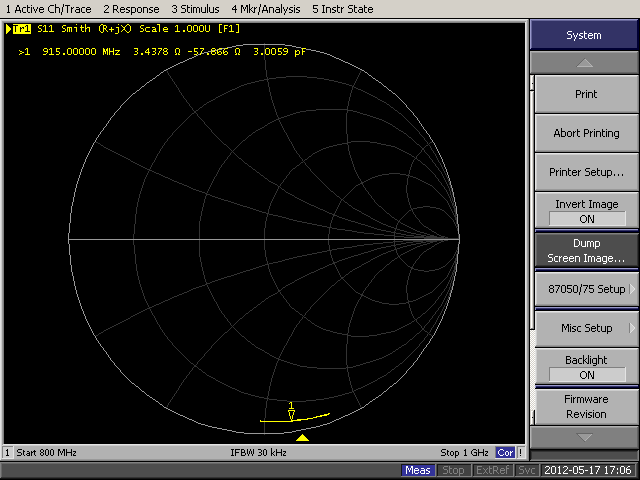
\includegraphics[width=5in]{Pictures/31May2012/CHIP_SALINE_AGILENTCAL_NOCORR} % requires the graphicx package
   \caption{NXP chip impedance in saline using the Agilent calibration kit, no manual calibration correction}
   \label{fig:chip_agilentcal_saline}
\end{figure}

The impedance of the NXP chip in the saline for this scenario at 915 MHz is $Z=3.4378 - j57.866 \, \Omega$, which is equivalent to a capacitance of 3.0059 pF.


\subsection{Small Loop Impedance in Saline Using Agilent Cal}
\indent \indent The impedance of the small loop using the calibration described above is shown below in Figure \ref{fig:loop_agilentcal_saline}. The power level is again set to -10.5 dBm.

\begin{figure}[htbp]
   \centering
   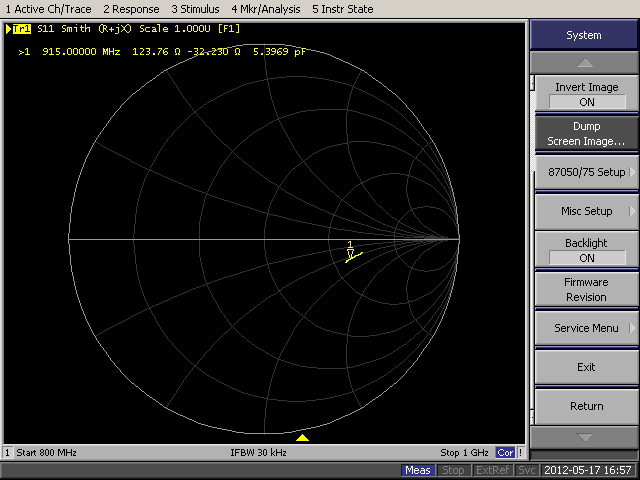
\includegraphics[width=5in]{Pictures/31May2012/LOOP_SNGL_TURN_SALINE_AGILENTCAL_NOCORR} % requires the graphicx package
   \caption{Small loop impedance in saline using the Agilent calibration kit, no manual calibration correction}
   \label{fig:loop_agilentcal_saline}
\end{figure}

The impedance of the small loop in the saline for this scenario at 915 MHz is $Z=123.76 - j32.230 \, \Omega$, which is equivalent to a capacitance of 5.3969 pF.


\subsection{Matching NXP Tag Chip in Saline to 50 $\Omega$}
\indent \indent Using the impedance matching network designer (\url{http://bwrc.eecs.berkeley.edu/research/rf/projects/60ghz/matching/impmatch.html}), the following 2 matching networks shown in Figures \ref{fig:Chip_saline_agilentcal_match1} and \ref{fig:Chip_saline_agilentcal_match2} were determined and then built using the same type of coaxial connector used for testing. 

\begin{figure}[h!]
	\centering
	\subfigure[Matching network 1: Lowpass Hi-low]{
	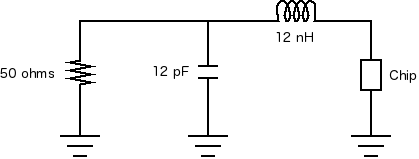
\includegraphics[width=2.8in]{Pictures/31May2012/Chip_saline_agilentcal_match1} 
	\label{fig:Chip_saline_agilentcal_match1}
	}
	\subfigure[Matching network 2: Highpass Low-hi]{
	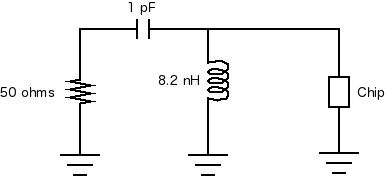
\includegraphics[width=2.8in]{Pictures/31May2012/Chip_saline_agilentcal_match2} 
	\label{fig:Chip_saline_agilentcal_match2}
	}
	\label{fig:Chip_saline_agilentcal_match}
	\caption{Matching networks for the NXP tag chip}
%	\caption[Optional caption for list of figures]{Backscattered signal strength as a function of
%	distance in the saline proxy for various carrier frequencies. Modulated backscatter of 
%	7.5 MHz in \subref{fig:backscatter_f75}, 15MHz in \subref{fig:backscatter_f15}, and 
%	30 MHz in \subref{fig:backscatter_f30}.}
\end{figure}


The resulting impedance with the addition of the matching networks is shown below in Figures \ref{fig:Chip_saline_agilentcal_match1_smithchart} and \ref{fig:Chip_saline_agilentcal_match2_smithchart}. The power level is -10.5 dBm.

\begin{figure}[h!]
	\centering
	\subfigure[Smith chart, matching network 1: Lowpass Hi-low]{
	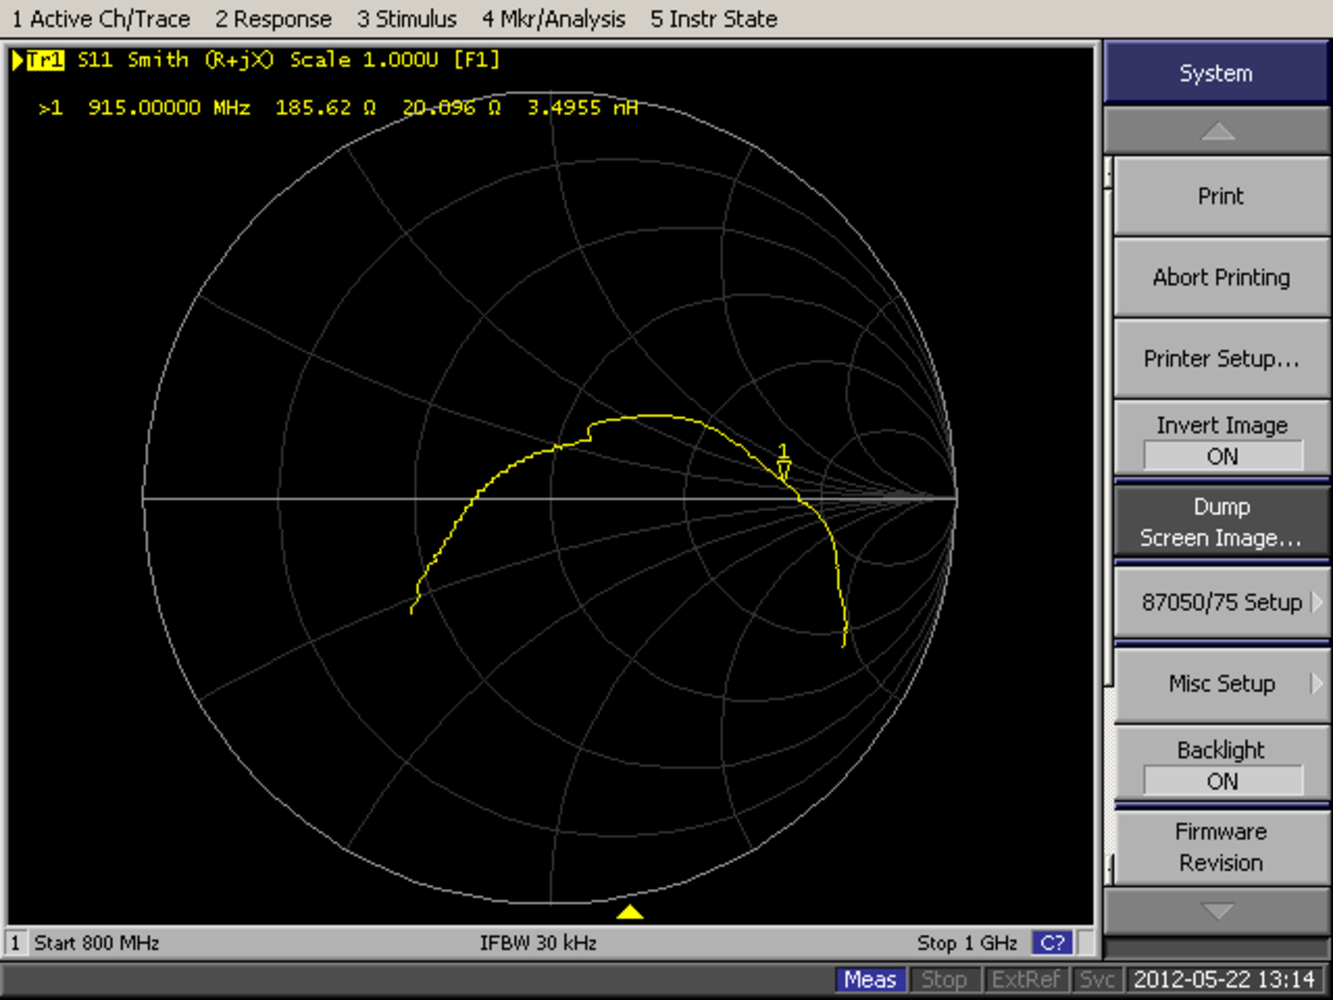
\includegraphics[width=2.8in]{Pictures/31May2012/CHIP_SALINE_MATCH_AGILENTCAL_NOCORR} 
	\label{fig:Chip_saline_agilentcal_match1_smithchart}
	}
	\subfigure[Smith chart, matching network 2: Highpass Low-hi]{
	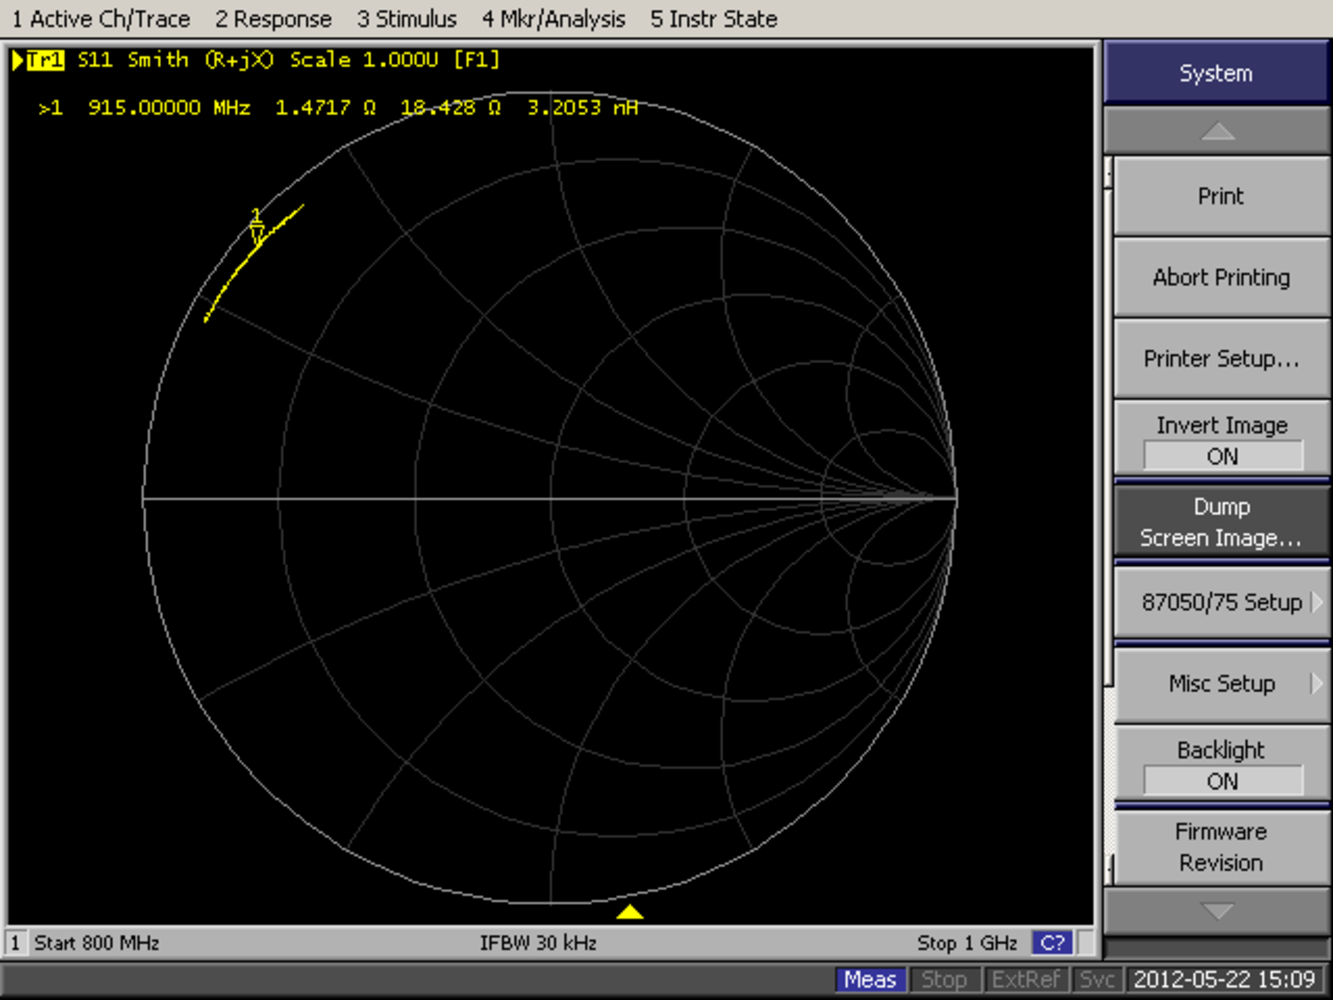
\includegraphics[width=2.8in]{Pictures/31May2012/CHIP_SALINE_MATCH2_AGILENTCAL_NOCORR} 
	\label{fig:Chip_saline_agilentcal_match2_smithchart}
	}
	\label{fig:Chip_saline_agilentcal_match_smithchart}
	\caption{Resulting impedance using matching networks for the NXP tag chip}
%	\caption[Optional caption for list of figures]{Backscattered signal strength as a function of
%	distance in the saline proxy for various carrier frequencies. Modulated backscatter of 
%	7.5 MHz in \subref{fig:backscatter_f75}, 15MHz in \subref{fig:backscatter_f15}, and 
%	30 MHz in \subref{fig:backscatter_f30}.}
\end{figure}

The impedance using the first matching network at 915 MHz is $Z=185.62+j20.096 \, \Omega$, which is equivalent to an inductance of 3.4955 nH. The second matching network at 915 MHz is $Z=1.4717+j18.428 \, \Omega$, which is equivalent to 3.2053 nH.



\subsection{Matching Small Loop in Saline to 50 $\Omega$}
\indent \indent The matching networks shown in Figures \ref{fig:Chip_saline_agilentcal_match1_smithchart} and \ref{fig:Chip_saline_agilentcal_match2_smithchart} were used.

\begin{figure}[h!]
	\centering
	\subfigure[Matching network 1: Lowpass Low-hi]{
	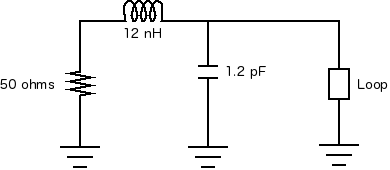
\includegraphics[width=2.8in]{Pictures/31May2012/Loop_sngl_turn_saline_agilentcal_match1.png} 
	\label{fig:Loop_sngl_turn_saline_agilentcal_match1}
	}
	\subfigure[Matching network 2: Highpass Low-hi]{
	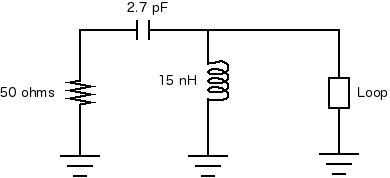
\includegraphics[width=2.8in]{Pictures/31May2012/Loop_sngl_turn_saline_agilentcal_match2.png} 
	\label{fig:Loop_sngl_turn_saline_agilentcal_match2}
	}
	\label{fig:Loop_sngl_turn_saline_agilentcal_match}
	\caption{Matching networks for the small loop}
%	\caption[Optional caption for list of figures]{Backscattered signal strength as a function of
%	distance in the saline proxy for various carrier frequencies. Modulated backscatter of 
%	7.5 MHz in \subref{fig:backscatter_f75}, 15MHz in \subref{fig:backscatter_f15}, and 
%	30 MHz in \subref{fig:backscatter_f30}.}
\end{figure}

The resulting impedance with the addition of the matching networks is shown below in Figures \ref{fig:LOOP_SNGL_TURN_SALINE_AGILENTCAL_MATCH1_NOCORR_smithchart} and \ref{fig:LOOP_SNGL_TURN_SALINE_AGILENTCAL_MATCH2_NOCORR_smithchart}

\begin{figure}[h!]
	\centering
	\subfigure[Smith chart, matching network 1: Lowpass Low-hi]{
	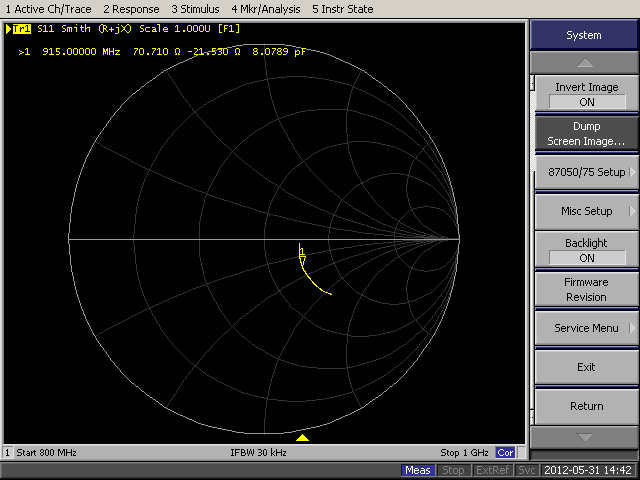
\includegraphics[width=2.8in]{Pictures/31May2012/LOOP_SNGL_TURN_SALINE_AGILENTCAL_MATCH1_NOCORR} 
	\label{fig:LOOP_SNGL_TURN_SALINE_AGILENTCAL_MATCH1_NOCORR_smithchart}
	}
	\subfigure[Smith chart, matching network 2: Highpass Low-hi]{
	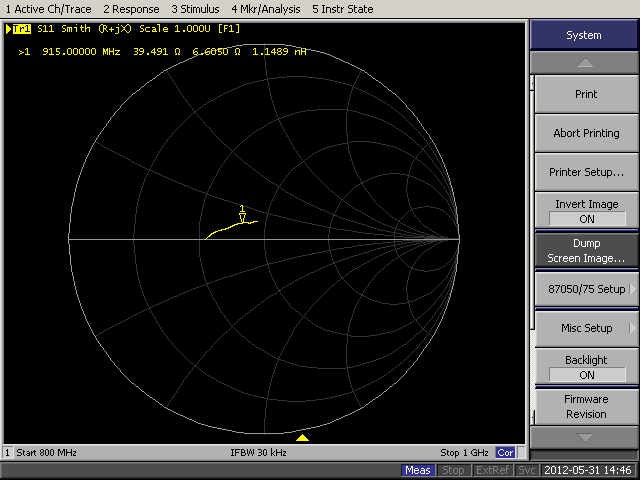
\includegraphics[width=2.8in]{Pictures/31May2012/LOOP_SNGL_TURN_SALINE_AGILENTCAL_MATCH2_NOCORR} 
	\label{fig:LOOP_SNGL_TURN_SALINE_AGILENTCAL_MATCH2_NOCORR_smithchart}
	}
	\label{fig:LOOP_SNGL_TURN_SALINE_AGILENTCAL_MATCH_NOCORR_smithchart}
	\caption{Resulting impedance using matching networks for the NXP tag chip}
%	\caption[Optional caption for list of figures]{Backscattered signal strength as a function of
%	distance in the saline proxy for various carrier frequencies. Modulated backscatter of 
%	7.5 MHz in \subref{fig:backscatter_f75}, 15MHz in \subref{fig:backscatter_f15}, and 
%	30 MHz in \subref{fig:backscatter_f30}.}
\end{figure}

The impedance using the first matching network at 915 MHz is $Z=70.710-j21.530 \, \Omega$, which is equivalent to a capacitance of 8.0789 nH. The second matching network at 915 MHz is $Z=39.491+j6.6050 \, \Omega$, which is equivalent to 1.1489 nH. While these 2 matching networks do not work perfectly to match the small loop to 50 $\Omega$, it appears that they are close enough, especially for the 2nd matching network, since the close proximity of the components can explain any parasitic capacitance and small wire lengths/solder blobs/slightly incorrect placement can potentially create parasitic inductance. 


%February 18, 2013-----------------------------------------------------------------------------------------------------------------------------------------
\clearpage
\section{18 February 2013:}

\indent \indent Today focused on fixing up some plots from last week's groupmeeting referring to comparing receiver architectures, as well as taking new data using the implantable setup in the tank of saline. Previously, to compare analog front-ends (AFE) of the receiver, the ratio between the self-jammer and the data sidebands was compared among different architectures, but the data sideband power was taken directly at the subcarrier frequency. But, when looking at the return signal power vs. distance, the total power in the sidebands was considered, so in order to be fair and consistent, the total power in the sideband(s) must be considered when comparing receiver architectures. When taking new data, with any receiver architecture employing a self-jammer canceler, it must be retuned for every distance/scenario.

\subsection{Comparing Receiver Architecture Analog Front Ends (AFE)}
\indent \indent To compare different receiver architectures, the metric used here is the difference between the self-jamming signal, the carrier, and the total power in the upper data sideband (USB). This ratio is in dBc, the difference between the total power in the upper sideband and that of the self-jammer. The better this ratio, the better the receiver architecture. Three (3) different analog front ends (AFE) for the receiver were considered here and are compared below.

\subsubsection{Circulator Architecture}
\indent \indent Figure \ref{fig:circulator_Rx_architecture} below shows the circulator based receiver architecture. A circulator is used instead of a coupler to decouple the Rx and Tx paths, and allows for higher sideband return strength, but at the cost of higher self-jammer signal as well. Part of the Tx signal only, ie: without data from the tag, is siphoned off the Tx path, shifted and attenuated, and then added to the return signal in an attempt to cancel out part of the return self-jamming signal for better SNR at the receiver.

Figure \ref{fig:alt_Rx_architecture_canceler} shows the envelope of the return signal using the spectrum analyzer, NOT at baseband. The signal is recorded both with and without the self-jammer canceler, to quantify the amount of rejection the self-jammer canceler is able to achieve. 

Table \ref{tab:alt_Rx_architecture_rejection} shows the total power in the upper sideband, the power in the self-jammer (carrier), and finally the rejection ratio, defined here as the difference between the total upper sideband power and the self-jammer. This ratio tells us how far below the self-jammer the total upper sideband power is, and is the metric for the effectiveness of the self-jammer canceler.

For the circulator architecture, it's clear that the self-jammer is reduced with the canceler by about 7 dBm, but the total power in the upper sideband decreased by about the same amount, such that the rejection ratio for both cases is essentially the same, rendering this architecture not useful as a self-jammer canceler for the receiver front end.

\begin{figure}[ht]
	\centering
	\subfigure[Circulator receiver architecture for analog front end (AFE)]{
		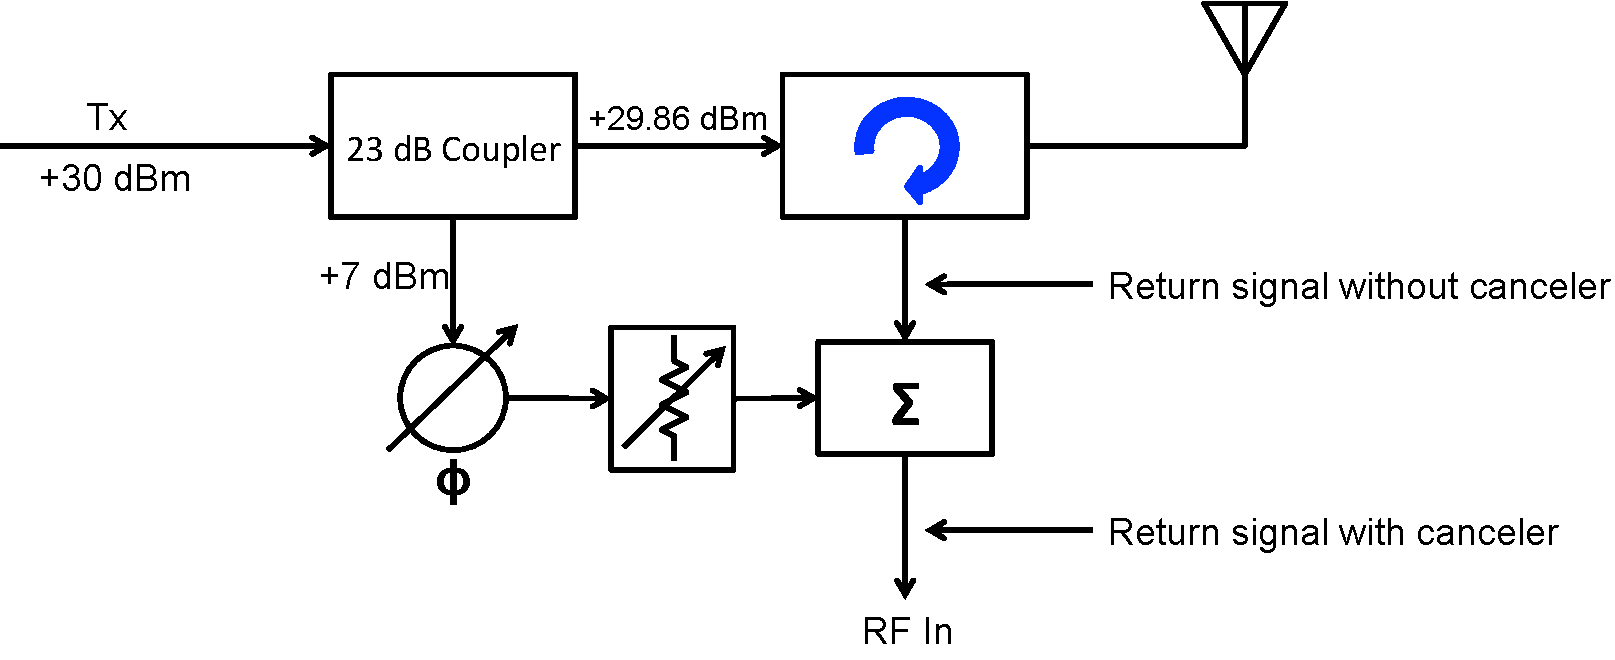
\includegraphics[width=0.45\textwidth]{Pictures/18Feb2013/alt_Rx_architecture}
		\label{fig:circulator_Rx_architecture}
		}
		\quad
	\subfigure[Return signal using circulator based receiver architecture with and without self-jammer canceler]{
		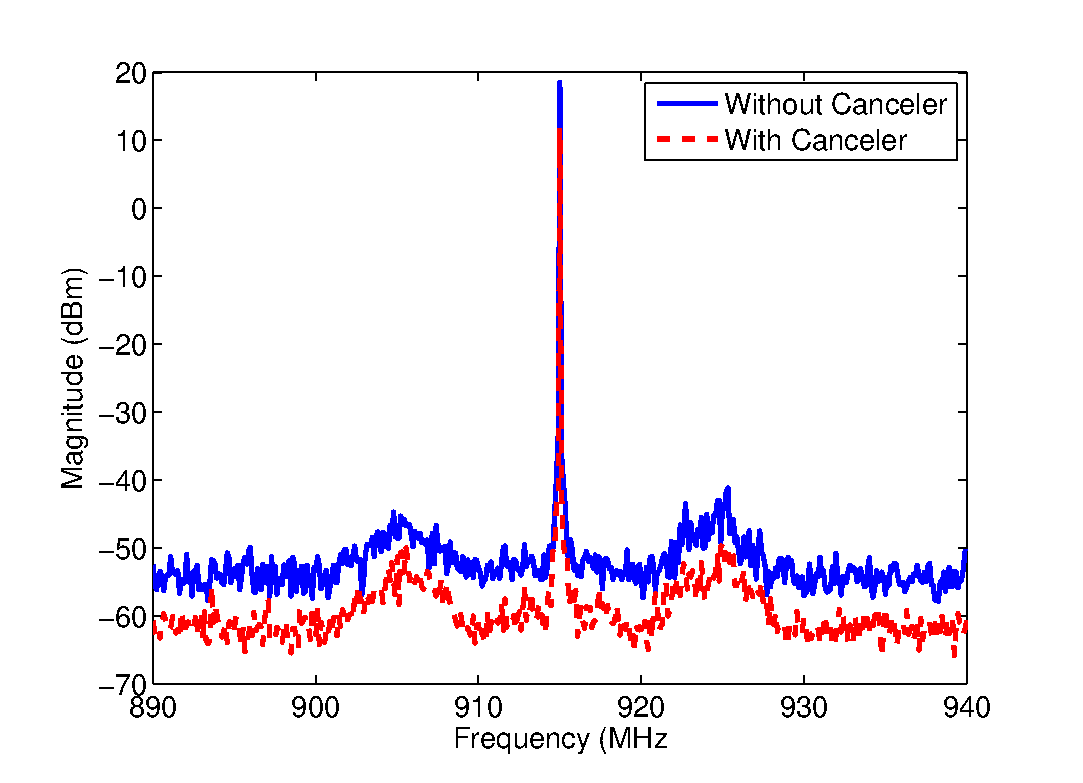
\includegraphics[width=0.45\textwidth]{Pictures/18Feb2013/alt_Rx_architecture_canceler} 
		\label{fig:alt_Rx_architecture_canceler}
		}
	\label{fig:alt_Rx}
	\caption{Response of circulator based receiver architecture}
\end{figure}

%Rejection ratio table
\begin{table}[h!]
\centering
	\caption{Circulator based receiver architecture self-jammer canceler rejection ratios}
	\begin{tabular}{| c | c | c || c |}
	\hline
	 & USB total power & Self-jammer power  & USB rejection ratio  \\
	 & (dBm) & (dBm) & (dBc) \\ \hline
	 Without canceler & -18.86 & 18.56 & -37.42 \\ \hline
	 With canceler & -25.59 & 11.80 & -37.39 \\ \hline
	\end{tabular}
\label{tab:alt_Rx_architecture_rejection}
\end{table}


\subsubsection{23 dB Coupler Architecture}

Figure \ref{fig:23dB_coup_Rx_architecture} shows the 23 dB coupler based receiver architecture, Figure \ref{fig:orig_Rx_architecture_canceler_23dBcoup} shows the return envelope of the backscattered signal with the tag 1 cm away in saline both with and without the self-jammer canceler, and Table \ref{tab:orig_Rx_architecture_rejection_23dBcoup} shows the achieved rejection ratio with this architecture. 

This architecture clearly achieves a better rejection ratio than the circulator based architecture with the self-jammer canceler included, and there is a clear advantage in including the self-jammer canceler in this scenario, as it improves the rejection ratio by about 17 dB. However, since a 23 dB coupler is being used to separate Tx and Rx paths, the total power in the USB is much lower, by about 23 dB, as expected, without the self-jammer canceler included (where the couple-out port is terminated). When the self-jammer canceler is included, the total power in the upper sideband only decreases by about 2 dBm, but the self-jammer is reduced by about 18 dBm, leading to a rejection ratio of about -22 dBc.

\begin{figure}[ht]
	\centering
	\subfigure[23 dB coupler receiver architecture for analog front end (AFE)]{
		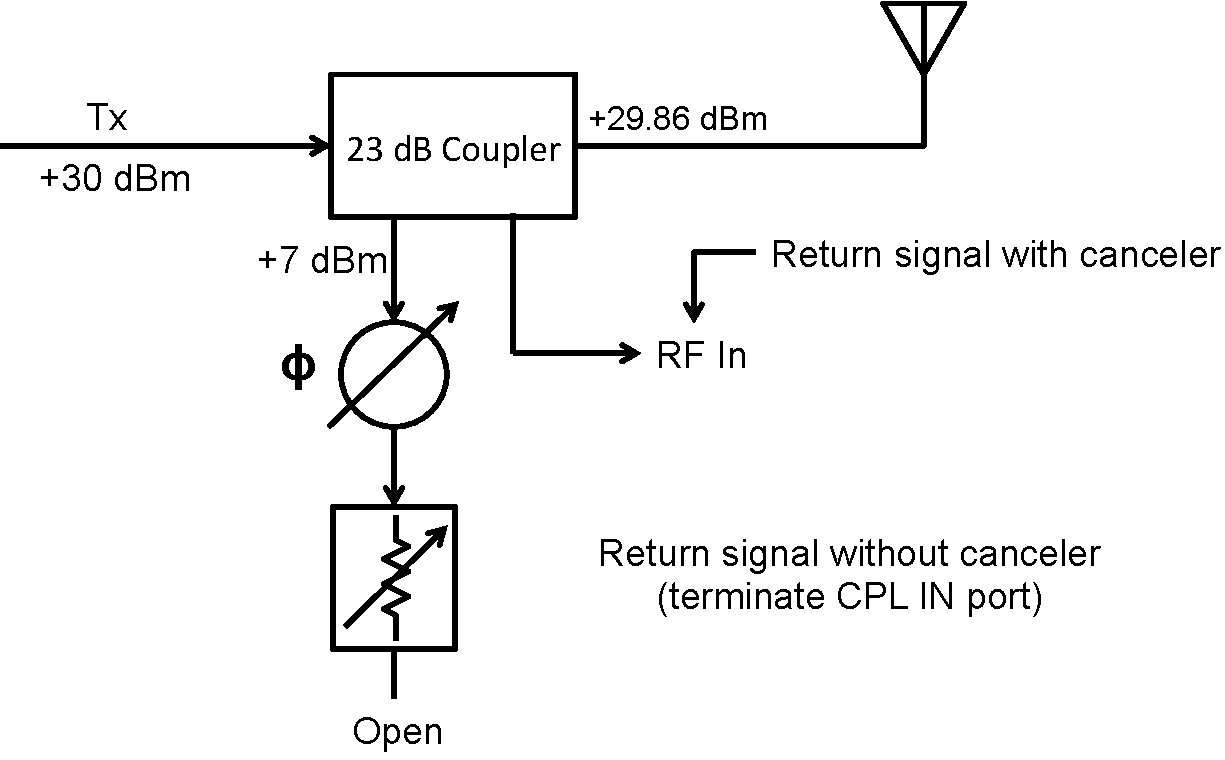
\includegraphics[width=0.45\textwidth]{Pictures/18Feb2013/orig_23dBcoup_Rx_architecture}
		\label{fig:23dB_coup_Rx_architecture}
		}
		\quad
	\subfigure[Return signal using 23 dB coupler based receiver architecture with and without self-jammer canceler]{
		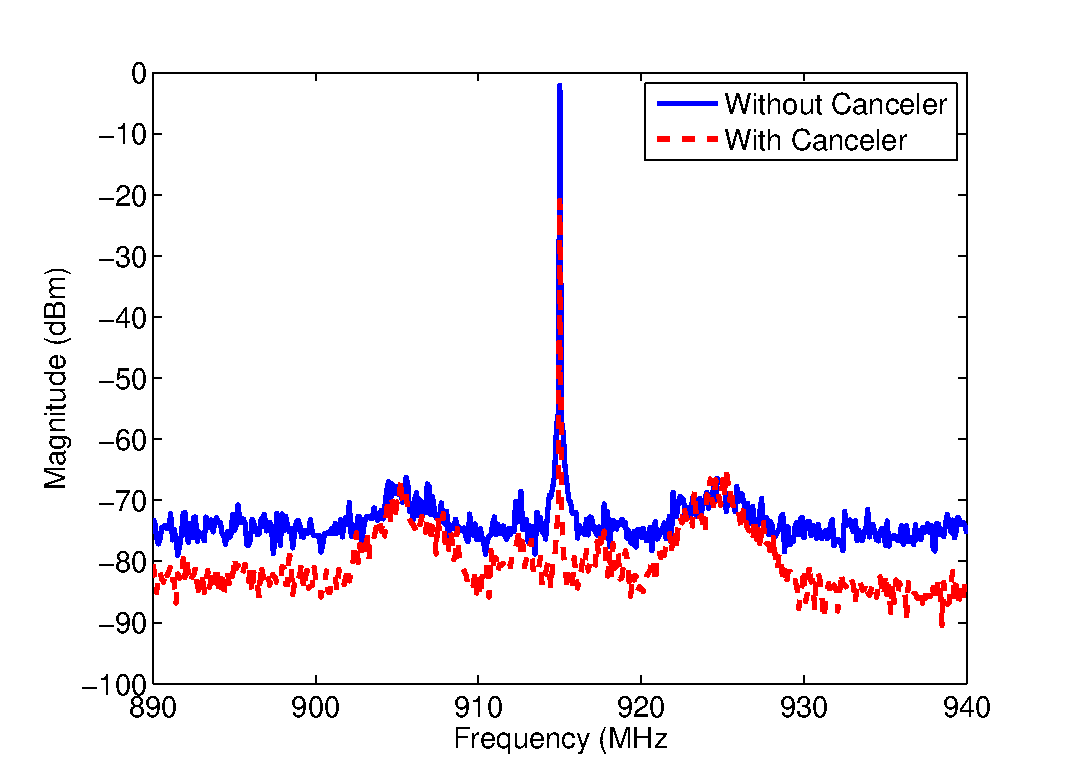
\includegraphics[width=0.45\textwidth]{Pictures/18Feb2013/orig_Rx_architecture_canceler_23dBcoup} 
		\label{fig:orig_Rx_architecture_canceler_23dBcoup}
		}
	\label{fig:orig_Rx_23dBcoup}
	\caption{Response of 23 dB coupler based receiver architecture}
\end{figure}

%Rejection ratio table
\begin{table}[h!]
\centering
	\caption{23 dB coupler based receiver architecture self-jammer canceler rejection ratios}
	\begin{tabular}{| c | c | c || c |}
	\hline
	 & USB total power & Self-jammer power  & USB rejection ratio  \\
	 & (dBm) & (dBm) & (dBc) \\ \hline
	 Without canceler & -41.56 & -2.14 & -39.42 \\ \hline
	 With canceler & -43.08 & -20.93 & -22.16 \\ \hline
	\end{tabular}
\label{tab:orig_Rx_architecture_rejection_23dBcoup}
\end{table}


\subsubsection{10 dB Coupler Architecture}

Figure \ref{fig:10dB_coup_Rx_architecture} shows the 10 dB coupler based receiver architecture, Figure \ref{fig:orig_Rx_architecture_canceler_10dBcoup} shows the return envelope of the backscattered signal with the tag 1 cm away in saline both with and without the self-jammer canceler, and Table \ref{tab:orig_Rx_architecture_rejection_10dBcoup} shows the achieved rejection ratio with this architecture. 

By replacing the 23 dB coupler in the previous architecture with a 10 dB coupler, it is expected that we will get back a stronger return signal from the tag but also a stronger self-jammer, and if the self-jammer can be reduced to a similar degree, the rejection ratio will be even better. This is indeed that case, as evidenced by the data in Table \ref{tab:orig_Rx_architecture_rejection_10dBcoup}. Without the self-jammer canceler, we achieve an extra 10 dBm in the upper sideband when compared to the 23 dB coupler, but the self-jammer is approximately 13 dBm stronger, leading to a similar rejection ratio without the self-jammer canceler. By including the self-jammer canceler and tuning it appropriately to achieve the best self-jammer suppression, the total power in the upper sideband decreases by about 2 dBm, but the self-jammer is suppressed by about 31 dBm, leading to a rejection ratio of about -10 dBc, a 12 dB improvement over the 23 dB coupler. 

This architecture using a 10 dB coupler instead of a 23 dB coupler is clearly the best receiver architecture in terms of the rejection ratio as defined here, however, while the inclusion of the coupler does allow for a better rejection ratio and SNR, it does decrease the available backscatter power, making it difficult for the back-end of the receiver to accurately demodulate the return signal. That is, even though the rejection ratio is good, which is a relative difference between self-jammer and signal power, the absolute power level of the return signal is lower and more difficult to demodulate.

An idea to overcome this low signal power would be to use an LNA on the return signal.

\begin{figure}[h!]
	\centering
	\subfigure[10 dB coupler receiver architecture for analog front end (AFE)]{
		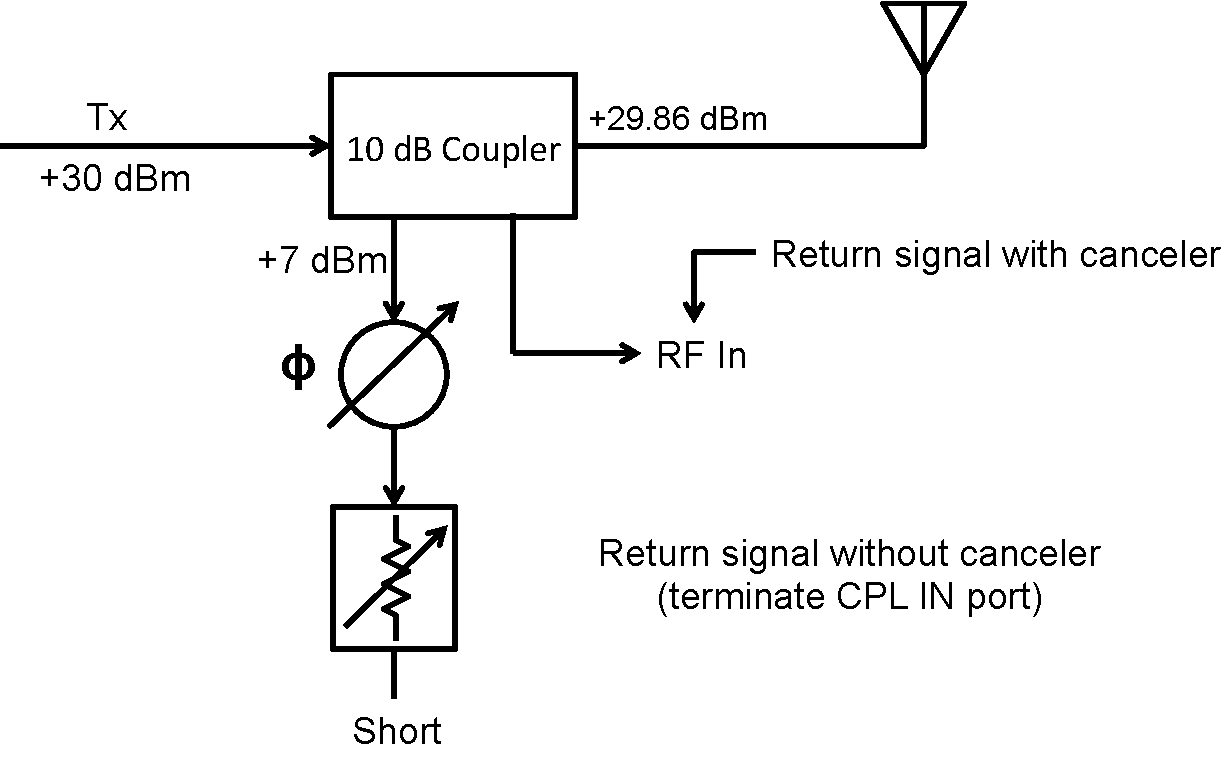
\includegraphics[width=0.45\textwidth]{Pictures/18Feb2013/orig_10dBcoup_Rx_architecture}
		\label{fig:10dB_coup_Rx_architecture}
		}
		\quad
	\subfigure[Return signal using 23 dB coupler based receiver architecture with and without self-jammer canceler]{
		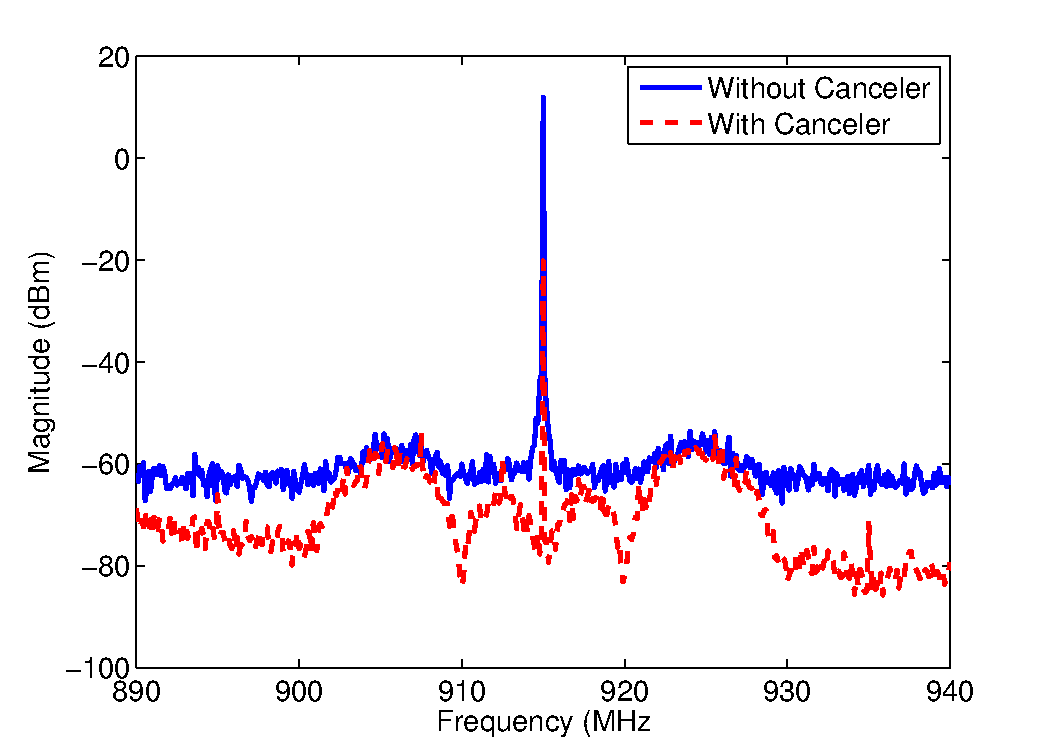
\includegraphics[width=0.45\textwidth]{Pictures/18Feb2013/orig_Rx_architecture_canceler_10dBcoup} 
		\label{fig:orig_Rx_architecture_canceler_10dBcoup}
		}
	\label{fig:orig_Rx_10dBcoup}
	\caption{Response of 10 dB coupler based receiver architecture}
\end{figure}

%Rejection ratio table
\begin{table}[h!]
\centering
	\caption{10 dB coupler based receiver architecture self-jammer canceler rejection ratios}
	\begin{tabular}{| c | c | c || c |}
	\hline
	 & USB total power & Self-jammer power  & USB rejection ratio  \\
	 & (dBm) & (dBm) & (dBc) \\ \hline
	 Without canceler & -28.64 & 11.87 & -40.50 \\ \hline
	 With canceler & -30.99 & -20.20 & -10.07 \\ \hline
	\end{tabular}
\label{tab:orig_Rx_architecture_rejection_10dBcoup}
\end{table}


%February 19, 2013-----------------------------------------------------------------------------------------------------------------------------------------
\clearpage
\section{19 February 2013:}

\indent \indent Today, I retook the data using the dragonfly tag in the saline tank. The receiver architecture shown in Figure \ref{fig:10dB_coup_Rx_architecture} was used, as this produced the best rejection ratio, shown in Table \ref{tab:orig_Rx_architecture_rejection_10dBcoup}. The self-jammer canceler was tuned at every tested distance to achieve the smallest magnitude self-jammer, boosting the rejection ratio as much as possible. The best rejection ratio was achieved with the self-jammer canceler attenuation at 5 dB, and the phase shifter was tuned in the middle of its full range. Since it's unknown how much of a phase shift is achievable with the currently used phase shifter, it might be worthwhile to switch to the trombone, as this will definitely give us at least 360 degrees of phase rotation.

In taking this data, the same measurements were recorded: $V_{reg}$, $V_{unreg}$, upper sideband power, and the entire backscatter envelope. The latter two measurements are automatically recorded using the equipment control software I wrote for the spectrum analyzer and signal generator. The measurements are shown below.

\subsection{Harvested Voltage}
\indent \indent The voltage harvested by the tag in the tank at each distance, where the self-jammer canceler has been tuned each time, is shown below in Figure \ref{fig:VHarvest_small_oct_loop_retune}.

\begin{figure}[h]
	\centering
	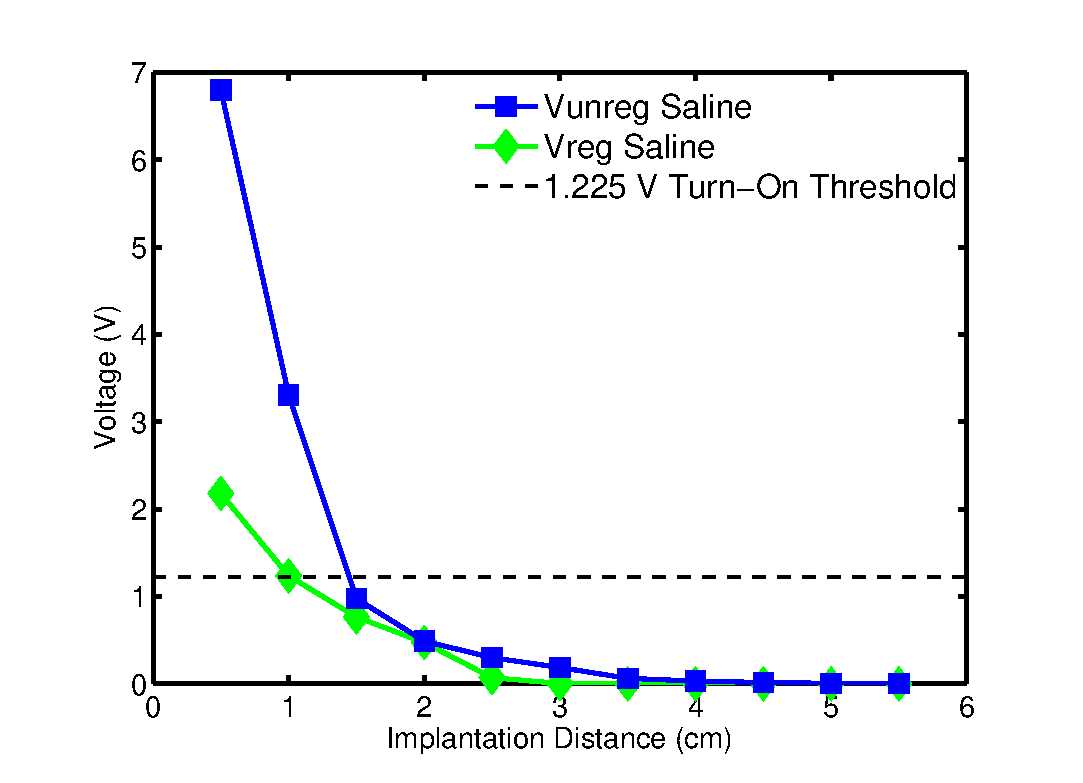
\includegraphics[width=0.6\textwidth]{Pictures/19Feb2013/VHarvest_small_oct_loop_retune}
	\caption{Harvested voltage from the ``implanted" tag in a tank of saline}
	\label{fig:VHarvest_small_oct_loop_retune}
\end{figure}

The tag only appears to harvest enough power to turn on and backscatter data up to a depth of about 1 to 1.5 cm, beyond this point, the tag does not harvest enough operating power. This maximum operating distance seems reduced when compared to previous tests. During this test, the small octagonal segmented loop was flipped so that it could be attached flush onto the tank containing the saline. However, in this setup with the flipped transceiver antenna, the transmit and receive signal must also travel through the FR-4 substrate, which is (find thickness!!!). This could account for the seemingly reduced harvested voltage, as well as the reduced maximum operating distance.

\subsection{Return Signal Strength}
\indent \indent The return signal strength of the backscattered data was also measured using the same setup as mentioned in the previous section. The strength of the return signal was calculated by determining the power in the upper sideband, from 920 - 930 MHz since there is a 10 MHz subcarrier for a data rate of 5 Mbps, and the 10 dB coupling loss was added back in, resulting in the power of the upper sideband of the return signal reference to the face of the antenna (not taking the antenna's gain into account, as that is unknown here! It can't be more than a dB or two, if that, due to its size and geometry). In calculating the power in the upper sideband, the resolution bandwidth setting of the spectrum analyzer was taken into account to remove frequency smearing over each sweep which would result in overestimating the measured power. This data is shown below in Figure \ref{fig:return_signal_strength_small_oct_loop_retune}.

\begin{figure}[h]
	\centering
	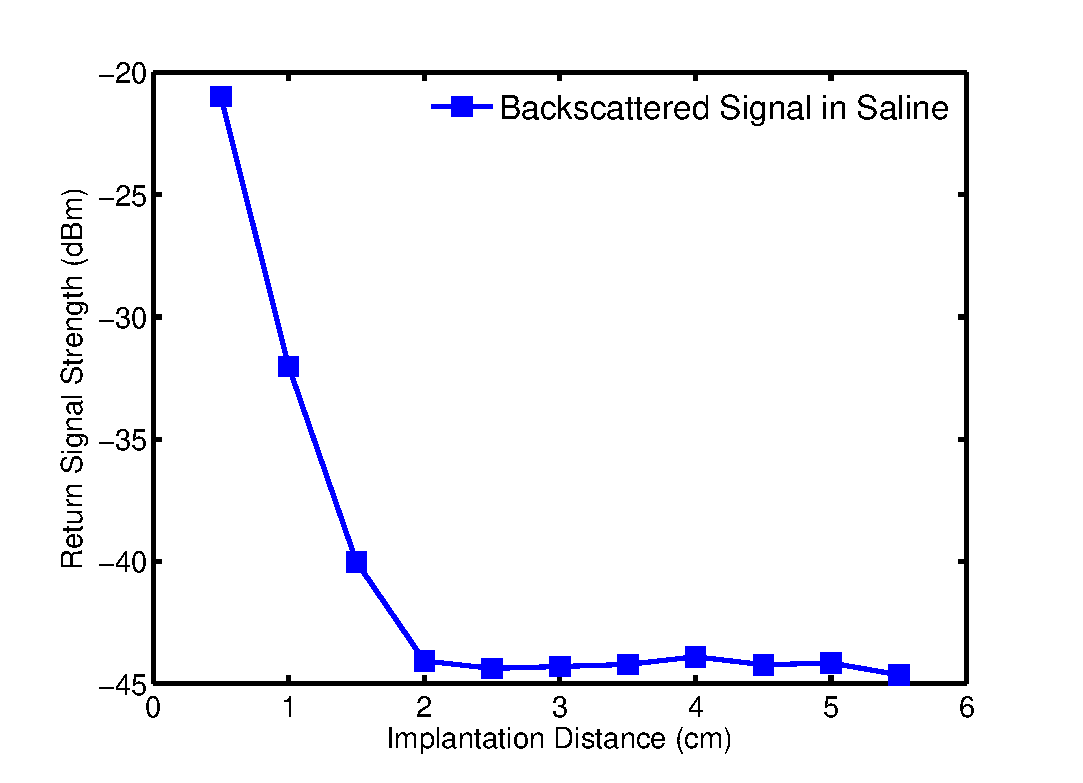
\includegraphics[width=0.6\textwidth]{Pictures/19Feb2013/return_signal_strength_small_oct_loop_retune}
	\caption{Return signal strength referenced to transceiver antenna}
	\label{fig:return_signal_strength_small_oct_loop_retune}
\end{figure}

Once the tag is moved to a distance of 2 cm, the return signal becomes buried in the noise floor of the spectrum analyzer, as shown by the essentially flat line in return signal strength at this distance and beyond. From 0.5 - 1.5 cm, the backscatter envelope is clearly visible, but drops below -35 dBm beyond 1 cm. Also, since this data is taking the coupling loss into account, the power levels seen by the receiver are 10 dBm lower, requiring  a sensitive receiver if a clean, accurate signal is to be demodulated. This further highlights the need for a sensitive receiver, as well as the benefit an LNA could provide.

\subsection{Rejection Ratio}
\indent \indent Here, we're looking at the achieved rejection ratio, as defined previously, of the self-jammer canceler at each distance. Again, the self-jammer canceler was tuned at each distance individually to achieve the best possible rejection ratio. The achieved rejection ratio versus distance is shown below in Figure \ref{fig:rejection_ratio_retune}.

\begin{figure}[h]
	\centering
	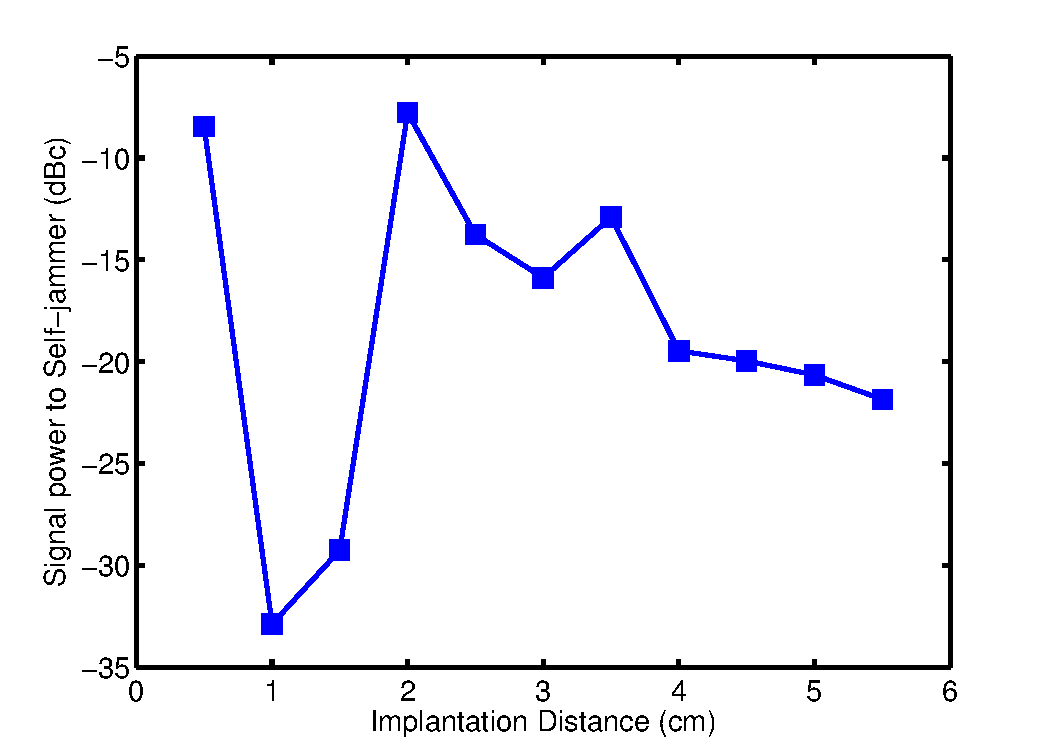
\includegraphics[width=0.6\textwidth]{Pictures/19Feb2013/rejection_ratio_retune}
	\caption{Rejection ratio of self-jammer canceler at each distance}
	\label{fig:rejection_ratio_retune}
\end{figure}

The rejection ratio achieved here before the return signal gets lost in the spectrum analyzer's noise appears to average about -20 dBc. One obvious feature here is the clear dip in the rejection ratio at 1 and 1.5 cm. I'm not 100\% sure why this happens yet, but judging from the return spectrum at those distances, it appears that even though the self-jammer is weaker at these distances with the canceler tuning, the upper sideband power decreases by a greater degree, leading to the degradation in the rejection ratio. Once a distance of 2 cm is reached, the sidebands are weaker, but the self-jammer is able to reduce the carrier signal to a further degree than the sideband level decreases, leading to a significantly better rejection ratio. Beyond 2 cm, the return signal is buried in the noise floor of the spectrum analyzer as seen in Figure \ref{fig:return_signal_strength_small_oct_loop_retune}, so the rejection ratio here doesn't grant us any information.


%February 20, 2013-----------------------------------------------------------------------------------------------------------------------------------------
\clearpage
\section{20 February 2013:}

\indent \indent Today is a group meeting day, so the morning was spent making slides to present. They consist of the data collected over the last couple days concerning the performance of the self-jammer canceler as well as the data collection with the tag in the tank making sure to retune the self-jammer canceler at every distance. I did have a chance to test out adding an amplifier to the Rx path and see how it affected the received backscatter envelope, as well as the self-jammer rejection ratio.

\subsection{Using an LNA to Increase Backscatter Signal Strength}
\indent \indent The receiver architecture using the 10 dB coupler is the best choice based on the rejection ratio, however, since we're using a 10 dB coupler to separate the Tx and Rx paths, the absolute power level of the data sidebands is still quite low, with the subcarrier power in the upper sideband of around -60 dBm (even though the total power in this sideband is around -30 dBm at a distance of 5 mm). 

To this end, I'm going to try using the {\textbf{ZRL-3500+}} low-noise amplifier from Mini-Circuits. It is advertised as an LNA, with a noise figure of 2.5 dB, and in the frequency range of 700 - 1600 MHz, it has a typical gain of 26 dB and a maximum output power of +24 dBm. The amplifier can accept a maximum input of +10 dBm, so since the self-jammer can reach levels above this while tuning the self-jammer canceler circuit, the self-jammer canceler should be tuned {\textbf{without}} the amplifier, and once it's certain that there are no components above or anywhere near +10 dBm, the amplifier can be connected. Since the amplifier is only capable of outputting a maximum of +24 dBm, there is no chance of damaging the spectrum analyzer, which has a maximum input power of +30 dBm.

Placing the tag about 1 cm away and tuning the self-jammer canceler without the amplifier in place, measuring the result and then placing the amplifier in place results in the backscatter envelope as shown below in Figure \ref{fig:BS_envelope_amplifier_comparison}. Table \ref{tab:BS_envelope_amplifier_comparison} shows the comparison between the two implementations.

\begin{figure}[h]
	\centering
	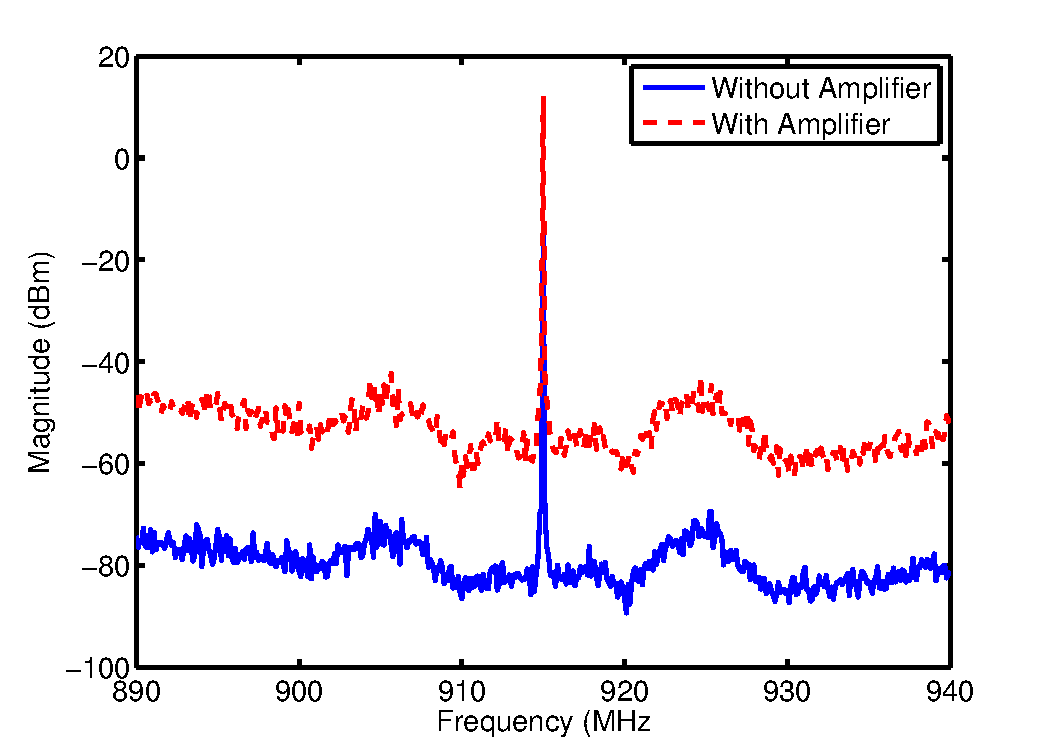
\includegraphics[width=0.6\textwidth]{Pictures/20Feb2013/BS_envelope_amplifier_comparison}
	\caption{Backscatter envelope with and without low-noise amplifier (LNA) on Rx path, self-jammer canceler included}
	\label{fig:BS_envelope_amplifier_comparison}
\end{figure}

%Rejection ratio table for amplifier
\begin{table}[h]
\centering
	\caption{Rejection ratio characteristics with and without a low-noise amplifier (LNA)}
	\begin{tabular}{| c | c | c || c |}
	\hline
	 & USB total power & Self-jammer power  & USB rejection ratio  \\
	 & (dBm) & (dBm) & (dBc) \\ \hline
	 Without amplifier & -46.79 & -15.20 & -31.59 \\ \hline
	 With amplifier & -20.33 & 12.09 & -32.42 \\ \hline
	\end{tabular}
\label{tab:BS_envelope_amplifier_comparison}
\end{table}

Not including an LNA on the Rx path, the receiver architecture appears as in Figure \ref{fig:10dB_coup_Rx_architecture}, and the resulting backscatter envelope is similar to that shown in Figure \ref{fig:orig_Rx_architecture_canceler_10dBcoup} and Table \ref{tab:orig_Rx_architecture_rejection_10dBcoup}. The tag in this experiment was placed at a distance of 1 cm instead of 0.5 cm for the previous investigation of the Rx architecture, which is why the total power in the USB is smaller by approximately 16 dBm. This also contributes to the worse rejection ratio when compared to the previous experiment. When the amplifier is added to the Rx path, the power in the USB increases by approximately 26 dB, and the power of the self-jammer (carrier) also increases by about 27 dB, right around the typical gain of the amplifier. Since both the power in the USB and the power of the self-jammer increase by nearly the same amount, the rejection ratio is nearly identical to the setup without the amplifier, only appearing 0.83 dB worse. 

Thus, since the rejection ratio is not essentially unaffected at the inclusion of an LNA on the Rx path, this may be a viable option for increasing the absolute power level of the backscattered data sidebands. However, one thing to note here is that the self-jammer is now approximately +12 dBm, which is a significant increase from its typical value of -15 dBm or smaller when the amplifier is not included, and this might affect the performance of the demodulator. While the SNR is within a couple dB when the amplifier is included, the demodulator might not be able to handle such a large self-jammer signal, potentially affecting its ability to cleanly reproduce the transmitted data. Moreover, a signal power of +12 dBm might damage the demodulator, and its maximum input power should be investigated before conducting any further experiments with the LNA in the full receiver.


%February 21, 2013-----------------------------------------------------------------------------------------------------------------------------------------
\clearpage
\section{21 February 2013:}

\indent \indent The plan for today is to examine the dragonfly tag chip to check for damage since the data I've been collecting with it has not matched up to data taken previously, and it appears that for the latest dataset shown in Figure \ref{fig:VHarvest_small_oct_loop_retune}, the harvested voltage is not regulated when the tag is 0.5 cm away and harvesting about 7 V. The regulated voltage here is above the 1.225 V threshold and appears to be approximately 2 V. 

Depending on the state of the tag, I have a couple Bug3 chips soldered onto the small boards, ready to be tested and matched if the original tag needs to be replaced. Also, the previous dataset was taken with the Tx antenna (small octagonal loop) flipped so that it could lie flush against the tank. There is a chance that this adversely affected the matching and performance of the antenna, causing the maximum distance for the ``implanted" tag to decrease from the original result of approximately 2.5 cm to 1.5 cm (marginally powered). The matching of the Tx antenna will be re-examined in both configurations to nail down the effect of flipping the antenna.

Once the chip is deemed ok, or once a new chip is made, data can be retaken (again). Another suggested test to run: semi-passive test. Power the chip with a battery so forward link is removed from equation, only looking at channel specifically, can get an idea of backscatter at further distances (much like was done for my 2012 RFID paper). 

\subsection{Testing for Chip Damage}
\indent \indent One quick method to test for damage to the chip, especially the regulator, is to inject a voltage into $V_{unreg}$ and measure and ensure that $V_{reg}$ is regulating the voltage properly.

Upon doing this, voltage regulation was achieved with $V_{unreg} \approx 1.4$ V. Regulation was maintained as shown in Figure \ref{fig:regulator_damage_test} below.

\begin{figure}[htbp]
	\centering
	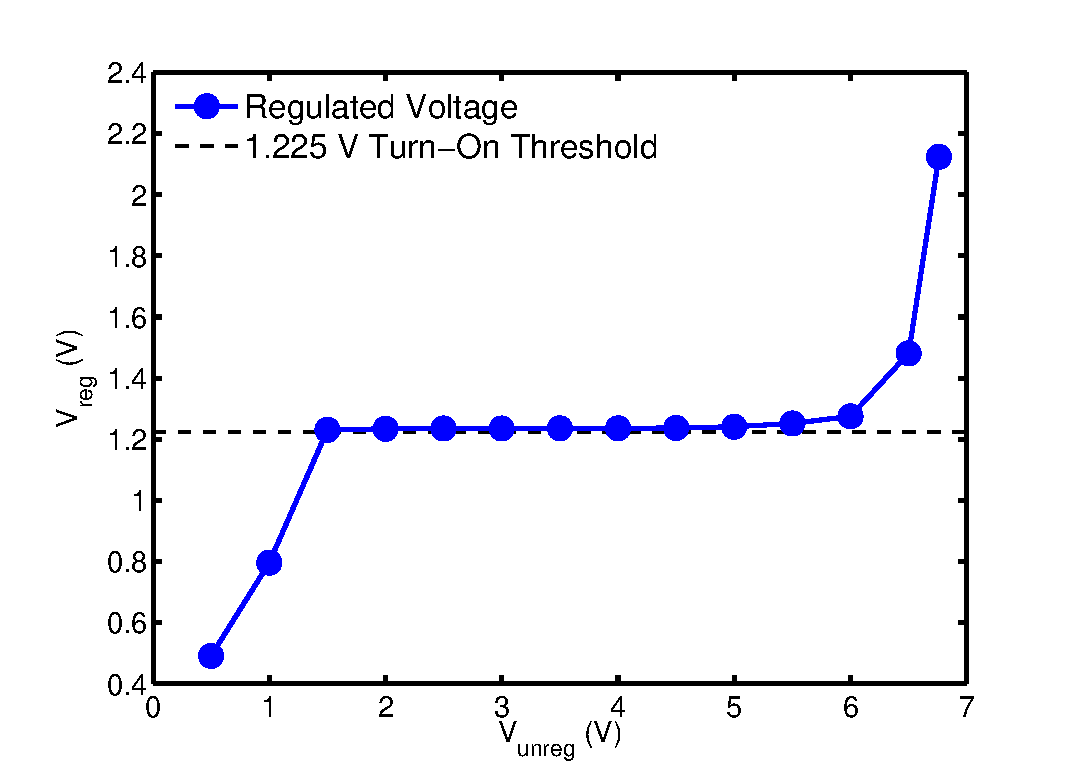
\includegraphics[width=0.6\textwidth]{Pictures/21Feb2013/regulator_damage_test}
	\caption{Regulator performance ($V_{reg}$) versus an injected ``harvested" voltage ($V_{unreg}$) }
	\label{fig:regulator_damage_test}
\end{figure}

As stated previously, the input voltage reaches regulation around a ``harvested" voltage of $\approx 1.4$ V, and regulation is maintained cleanly until $\approx 6.5$ V. When the unregulated, ``harvested" voltage reaches 6.5 V, the voltage supplied to the chip appears to no longer be regulated, as it is around 1.4 V here, and once the unregulated voltage reaches $\approx 6.76$ V, the regulated voltage is now $\approx 2.1$ V, much greater than the threshold of 1.225 V. 

The transistors in the chip are apparently only rated to about 5 V, which might explain the voltage supplied to the chip deviating from regulation beyond this point, namely around 6.5 V. However, in previous tests, the chip was able to maintain regulation for harvested voltages as high as 10 V. But, since this was the same chip that is being currently tested and used for data collection, it is possible that those previous and the current high harvested voltages might have contributed to burning out the chip.

Figures \ref{fig:Chip_in_glove} and \ref{fig:possible_MN_corrosion} show the chip inside and outside of the glove. The outline of the chip inside the glove is shown in Figure \ref{fig:Chip_in_glove}, and we can clearly see salt deposits near the top of the latex glove, as well as some discoloration of the glove where the chip is inside. Upon removing the chip from the glove, it appeared clean and dry, but placing it under the microscope revealed the closeup view in Figure \ref{fig:possible_MN_corrosion}, where it appears that there might be some slight corrosion or damage near the components of the matching network between the chip and small loop antenna.

\begin{figure}[T!]
	\centering
	\subfigure[Chip inside a latex glove, used to protect the chip from the saline]{
		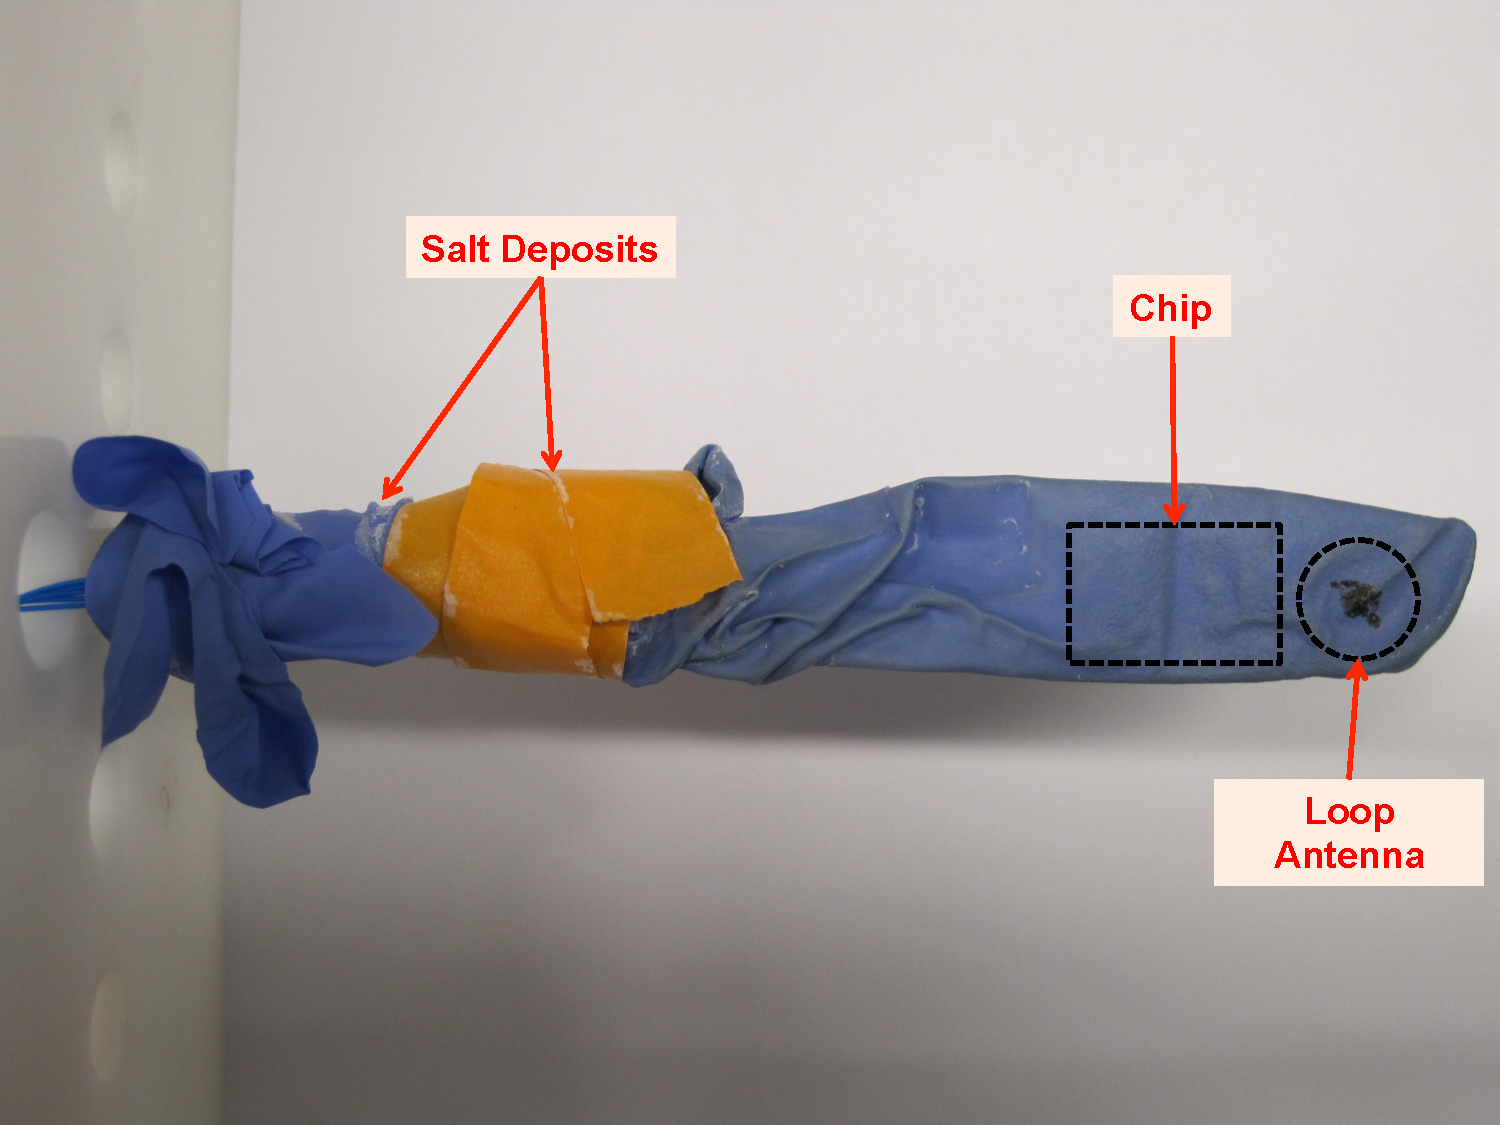
\includegraphics[width=0.45\textwidth]{Pictures/21Feb2013/Chip_in_glove}
		\label{fig:Chip_in_glove}
		}
		\quad
	\subfigure[Chip removed from latex glove and closeup showing possible corrosion]{
		\includegraphics[width=0.45\textwidth]{Pictures/21Feb2013/possible_MN_corrosion} 
		\label{fig:possible_MN_corrosion}
		}
	\label{fig:chip_damage_inspection}
	\caption{Inspecting the chip for possible damage}
\end{figure}

This was the only possible visible damage that could be detected. Judging by the data in Figure \ref{fig:regulator_damage_test} concerning the regulator and by inspecting the chip, there is a good chance that this chip is damaged to the point where switching to a new one is warranted. This is now the next step. I have soldered a couple new chips onto boards, and now I need to test them to make sure they work, and then match them. 

\subsection{Testing and Matching New Bug3 Chips}
\indent \indent For tomorrow...


%February 22, 2013-----------------------------------------------------------------------------------------------------------------------------------------
\clearpage
\section{22 February 2013:}

\indent \indent Today will focus on testing and matching a couple of new Bug3 chips, since the other day it was determined that the chip I've been using for testing is slightly damaged, possibly due to overloading some of the transistors with too much voltage? Either way, I have 2 new chips soldered onto the small boards, and they need to be confirmed as operational. In doing so, I can capture and save the chip's impedance characteristics over frequency and power using the control files for the network analyzer. This should make future matching of these chips easier.

If time allows, I can also measure the characteristics of the small loop antennas for the chips, and the effect of flipping the small octagonal segmented loop antennas on the tank.

\subsection{Testing and Matching New Bug3 Chips}
\indent \indent To ensure that the newly soldered Bug3 chips work, I had to check their impedance on the network analyzer. Since these chips are eventually going to be matched to a small loop antenna, calibration here is very important, namely the calibration plane, the spot on the circuitry that the network analyzer is calibrated to. If the calibration plane is off, the input impedance of the chip will be recorded incorrectly, as any extra path length will add impedance, capacitance, and resistance. 

Calibration was performed with a custom ``cal kit," consisting of the same small boards the chips are soldered onto, with an open, short ,and match ($50 \Omega$ load) right where the matching network will begin. The traces for the open, short, and match were saved and used for off-line calibration using vna\_calcorr.m. The impedance of both of the chips tested is shown in Figures \ref{fig:chip1_FS_impedance} and \ref{fig:chip2_FS_impedance}.

\begin{figure}[T!]
	\centering
	\subfigure[Impedance of chip \#1 in free space swept over power]{
		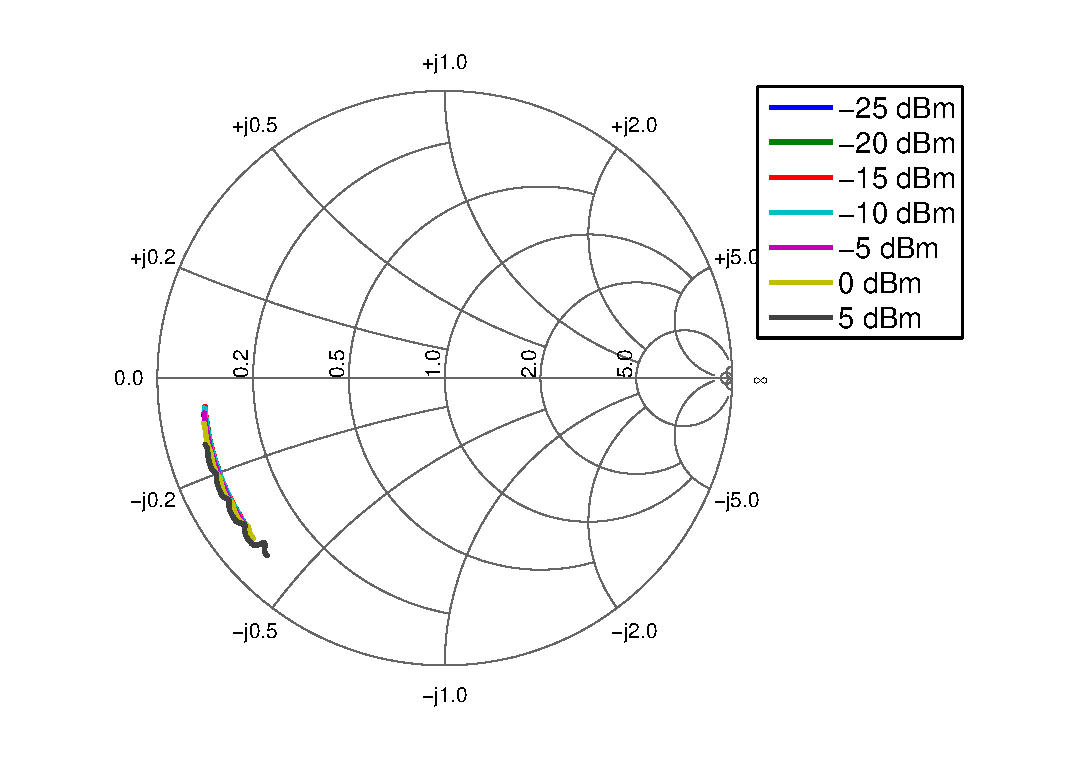
\includegraphics[width=0.45\textwidth]{Pictures/22Feb2013/chip1_FS_impedance}
		\label{fig:chip1_FS_impedance}
		}
		\quad
	\subfigure[Impedance of chip \#2 in free space, swept over power]{
		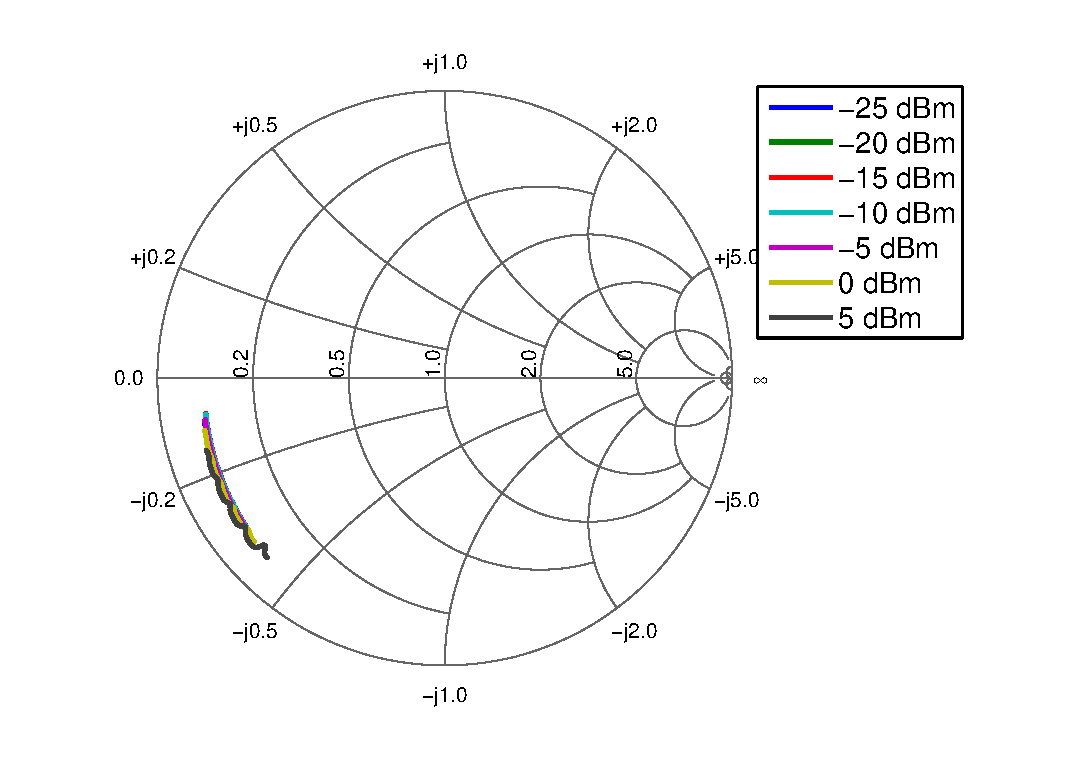
\includegraphics[width=0.45\textwidth]{Pictures/22Feb2013/chip2_FS_impedance} 
		\label{fig:chip2_FS_impedance}
		}
	\label{fig:chip_FS_impedance}
	\caption{Impedance of Bug3 chip in free space. Power swept from -25 dBm to +5 dBm, frequency from 800 MHz to 1 GHz}
\end{figure}

Since the chip includes an RF harvester, its impedance is power dependent due to the nonlinear diodes. As the power is swept from a low value, -25 dBm, up to a high value, +5 dBm, we can clearly see the shift in impedance and when the diodes become active and the harvester ``turns on." Both chips show a very similar impedance over the swept powers and frequencies, and in their current state without a matching network, both are poorly matched to 50 $\Omega$.

We're concerned about using the chip at approximately 915 MHz, so Table \ref{tab:chip_FS_impedance} shows the impedance, both real/imaginary and $R+jX$ form, for each chip at 915 MHz. Since determining the impedance of the chip is only a 1-port measurement, we can easily convert between real/imaginary and $R+jX$ forms using the definition of the load reflection coefficient, $\Gamma_{L}$, in equation \ref{equ:gamma_L}:

\begin{equation}
\label{equ:gamma_L}
\Gamma_{L} = \frac{Z_L - Z_S}{Z_L + Z_S}
\end{equation}

where $Z_L$ is the load impedance, the chip in this case, and $Z_S$ is the source impedance, $50 \Omega$ here, from the network analyzer. Solving for $Z_L$, we arrive at equation \ref{equ:Z_L}.

\begin{equation}
\label{equ:Z_L}
Z_L = Z_S \frac{1+\Gamma_L}{1-\Gamma_L}
\end{equation}

%Bug3 chip impedance in FS
\begin{table}[h]
\centering
	\caption{Bug3 chip impedance at 915 MHz in free space}
	\begin{tabular}{| c | c | c | c | c |}
	\hline
	& \multicolumn{2}{|c|}{Chip \#1} & \multicolumn{2}{|c|}{Chip \#2} \\ \hline
	 Power (dBm) & Real/Imag & $R+jX \, \Omega$ & Real/Imag & $R+jX \, \Omega$ \\ \hline
	 -25 &  $-0.8019-j0.2947$ & $4.052-j8.840 \, \Omega$ & $-0.7956-j0.3170$ & $4.008-j9.534 \, \Omega$ \\ \hline
	 -20 & $-0.8029-j0.2697$ & $4.252-j8.114 \, \Omega$ & $-0.7986-j0.2878$ & $4.211-j8.673 \, \Omega$ \\ \hline
	 -15 & $-0.8029-j0.2696$ & $4.253-j8.113 \, \Omega$ & $-0.7993-j0.2887$ & $4.184-j8.693 \, \Omega$ \\ \hline
	 -10 & $-0.8032-j0.2733$ & $4.211-j8.217 \, \Omega$ & $-0.7985-j0.2918$ & $4.176-j8.788 \, \Omega$\\ \hline
	 -5 & $-0.8013-j0.2940$ & $4.074-j8.826 \, \Omega$ & $-0.7969-j0.3110$ & $4.034-j9.350 \, \Omega$  \\ \hline
	 0 & $-0.7936-j0.3321$ & $3.905-j9.982 \, \Omega$ & $-0.7888-j0.3519$ & $3.820-j10.589 \, \Omega$ \\ \hline
	 5 & $-0.7702-j0.4137$ & $3.567-j12.518 \, \Omega$ & $-0.7657-j0.4275$ & $3.498-j12.954 \, \Omega$ \\ \hline
	\end{tabular}
\label{tab:chip_FS_impedance}
\end{table}

We're now going to try and match the Bug3 chip at an input power of 0 dBm at a frequency of 915 MHz, to a source frequency of 50 $\Omega$, to ensure that they're able to harvest energy and backscatter data properly. Choosing these numbers from Table \ref{tab:chip_FS_impedance}, we arrive at the...

To be continued...


%February 25, 2013-----------------------------------------------------------------------------------------------------------------------------------------
\clearpage
\section{25 February 2013:}

\indent \indent On Friday, I realized I made the mistake of forgetting to perform offline calibration of the chip impedance data before attempting to determine a matching network. Thus, the matching network did not work at all, as it was designed with an impedance that was incorrect. Table \ref{tab:chip_FS_impedance} has been corrected with the proper values of the chip impedance at varying power levels at 915 MHz. Matching and testing of the chip was performed, to ensure they work properly.


\subsection{Testing and Matching Bug3 Chips}
\subsubsection{Chip \#1}
Using the impedance data at 0 dBm input power, the matching network shown in Figure \ref{fig:Chip1_MN_schematic} was used (as suggested by Matt), and the resulting impedance on the Smith chart is shown in Figure \ref{fig:Chip1_MN_Smith} and the return loss in Figure \ref{fig:Chip1_MN_logmag}.


\begin{figure}[htbp]
	\centering
	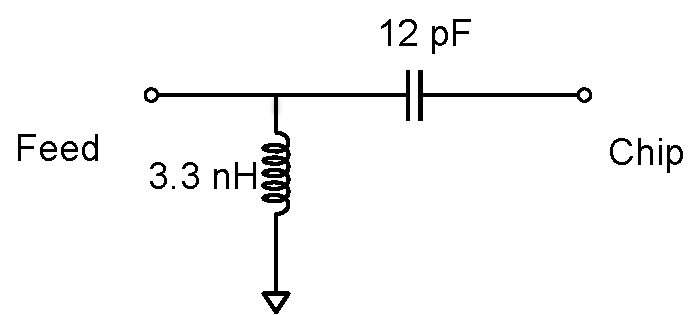
\includegraphics[width=0.6\textwidth]{Pictures/25Feb2013/Chip1_MN_schematic}
	\caption{Matching network used for Chip \#1 }
	\label{fig:Chip1_MN_schematic}
\end{figure}


\begin{figure}[htbp]
	\centering
	\subfigure[Impedance of chip \#1 with matching network]{
		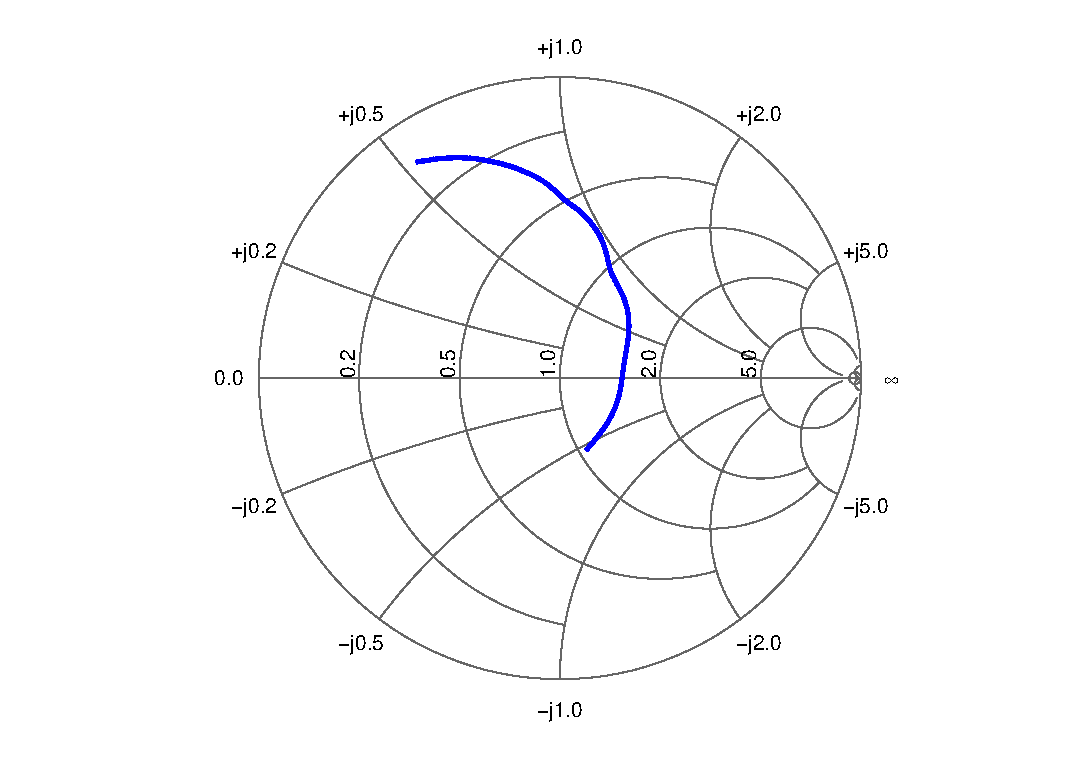
\includegraphics[width=0.45\textwidth]{Pictures/25Feb2013/Chip1_MN_Smith}
		\label{fig:Chip1_MN_Smith}
		}
		\quad
	\subfigure[Return loss of chip \#1 with matching network]{
		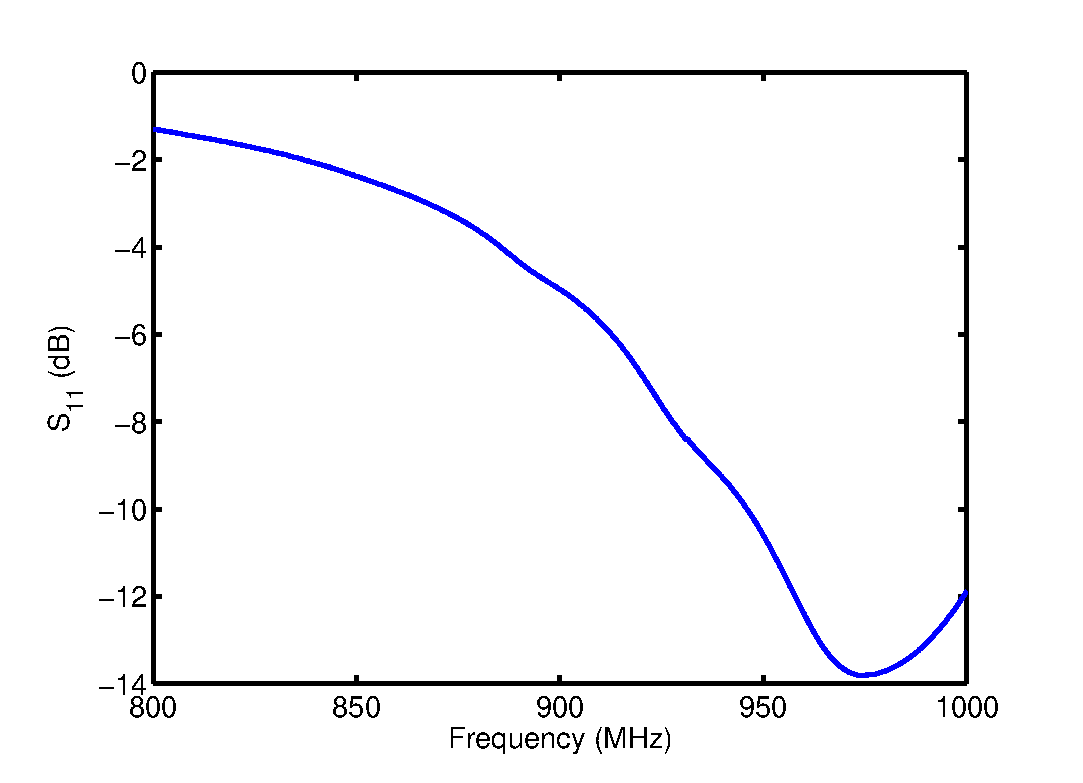
\includegraphics[width=0.45\textwidth]{Pictures/25Feb2013/Chip1_MN_logmag} 
		\label{fig:Chip1_MN_logmag}
		}
	\label{fig:Chip1_MN}
	\caption{Impedance and return loss of chip \#1 with matching network in place, input power set at 0 dBm}
\end{figure}

While the chip isn't matched perfectly at 915 MHz, it has a return loss of $\approx 13.82$ dB at about 975 MHz, which is good enough to test that it works and backscatters data properly.

Upon testing the chip in a cabled setup with the 10 dB coupler, it works!!! It backscatters data when the Tx power reaching the chip is between 4 - 6 dBm. Now to test the other chip...


\subsubsection{Chip \#2}
Using the same matching network for chip \#1 shown in Figure \ref{fig:Chip1_MN_schematic} at the same power level, we achieve a result very similar to that of chip \#1 (not shown here for brevity). The best match is achieved at a frequency of 972 MHz with a return loss of 13.42 dB. 

Testing this chip in the same cabeled setup at first produced no backscatter at all for similar threshold powers as chip \#1. Upon inspection of the chip on the board, it turns out that one of the pads of the 20 MHz crystal oscillator was not soldered in place. Soldering this pad down fixed the problem, and this chip works fine as well, and turns on at a similar threshold to chip \#1.

Now, these chips can be matched to small loop antennas in different scenarios.

\subsection{Impedance Characteristics of 9.5 mm Diameter Loop Antenna in Saline}
\indent \indent Using the customized ``cal kit" to determine the impedance of the small 9.5 mm single turn loop in the saline tank while it is soldered onto the same board as the chips (so it's calibrated to the same point) produces the results shown in Figures \ref{fig:sngl_loop_saline_smith} and \ref{fig:sngl_loop_saline_RL}.

\begin{figure}[htbp]
	\centering
	\subfigure[Smith chart]{
		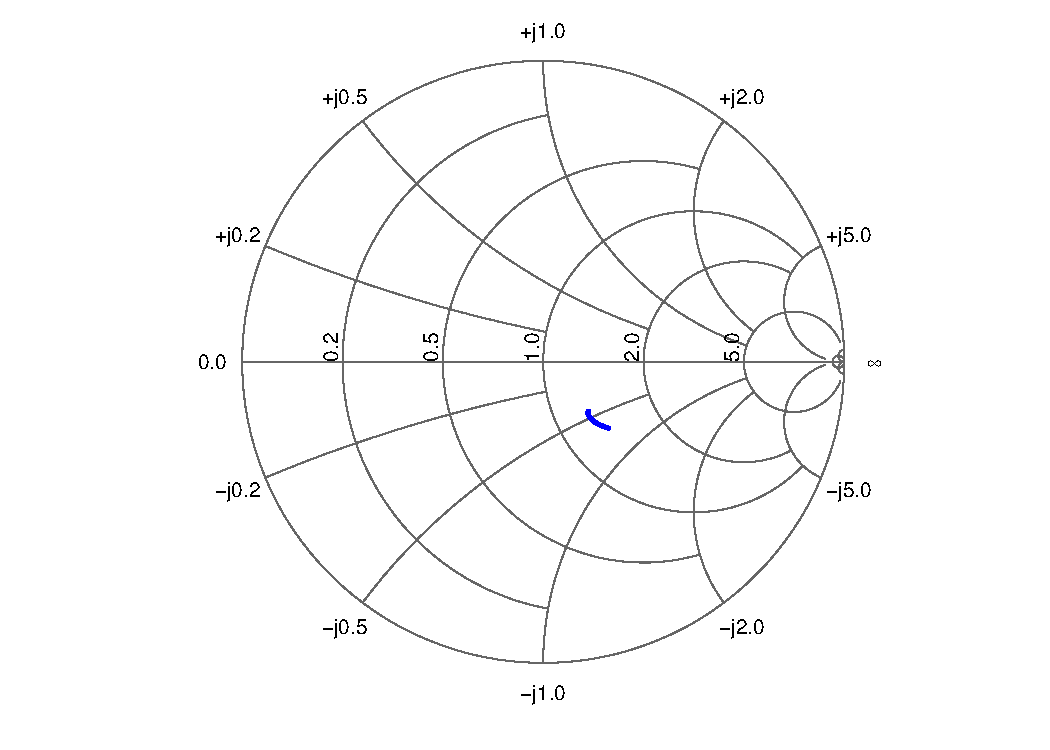
\includegraphics[width=0.45\textwidth]{Pictures/25Feb2013/sngl_loop_saline_smith}
		\label{fig:sngl_loop_saline_smith}
		}
		\quad
	\subfigure[Return loss]{
		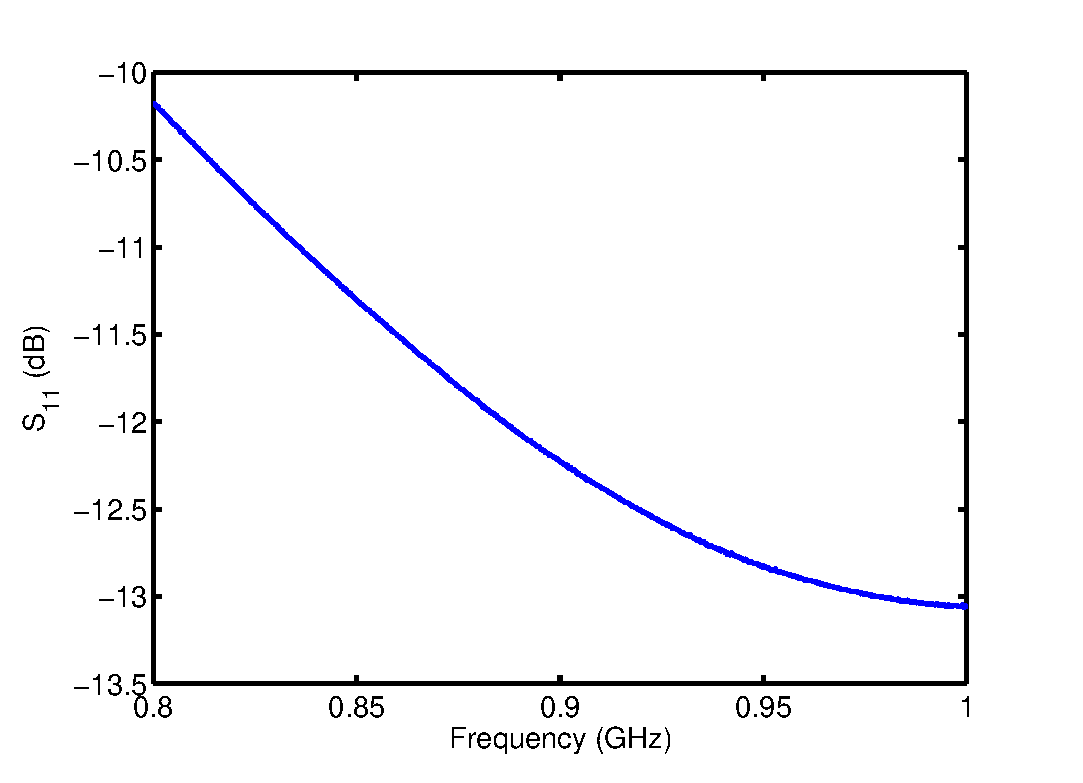
\includegraphics[width=0.45\textwidth]{Pictures/25Feb2013/sngl_loop_saline_RL} 
		\label{fig:sngl_loop_saline_RL}
		}
	\label{fig:sngl_loop_saline}
	\caption{Impedance and return loss of single turn 9.5 mm diameter loop}
\end{figure}

The impedance and return of the chip at 915 MHz, the frequency we care about and will match to, is shown in Table \ref{tab:sngl_loop_saline}. This is assuming a $50 \, \Omega$ source (ie: the VNA). The idea here is going to be to match the chip to the antenna's impedance for minimum reflections between the two. So, we're matching each component to the {\bf{conjugate}} of the other instead of matching each to $50 \, \Omega$, which is typically done as most antennas are $50 \, \Omega$ at the feed point. It was difficult to get the small loop to $50 \, \Omega$ previously, but now it appears to be quite close to that point when fully immersed in the saline {\bf{in a latex glove}}. When we move to either the silicone compound or the sugru for potting/waterproofing, this data will need to be reinvestigated, as the waterproofing material will affect the impedance, and thus the matching, of the antenna.

Surprisingly, submerging the small loop antenna in saline drastically improves its matching to a $50 \, \Omega$ source. In fact, its return loss with a $50 \, \Omega$ source over the tested range of 800 MHz to 1 GHz is entirely below 10 dB, indicating a good match. This is possibly due to the fact that when the poor radiating small loop is placed inside the saline, which is a very lossy, dielectric fluid when compared to free space, the wavelength of the injected signal decreases significantly, so the small loop appears electrically larger. Also, the small loop is less lossy when compared with the new surrounding media of the saline.

%Single 9.5 mm diameter loop impedance in saline at 915 MHz
\begin{table}[h]
\centering
	\caption{Impedance Characteristics of Single-turn 9.5 mm Diameter Loop in Saline at 915 MHz}
	\begin{tabular}{| c || c |}
	\hline
	$\Gamma_L$ & $0.153-j0.183$ \\ \hline
	$S_{11}$ & -12.4 dB \\ \hline
	$Z_L$ & $62.86-j24.38 \, \Omega$ \\ \hline
	\end{tabular}
\label{tab:sngl_loop_saline}
\end{table}

\subsection{Impedance Characteristics of Bug3 Chip in Saline}
\indent \indent Again, using the customized ``cal kit" to determine the impedance of the Bug3 chip in the tank of saline. New calibrations need to be recorded here, as everything must be submerged in saline for testing purposes. These measurements were recorded with everything inside a latex glove submerged in the tank of 0.91\% saline, containing about 6 L worth.

Figures \ref{fig:chip1_saline_impedance} and \ref{fig:chip2_saline_impedance} show the impedance of the chip in the tank of saline. 


\begin{figure}[htbp]
	\centering
	\subfigure[Impedance of chip \#1 in saline swept over power]{
		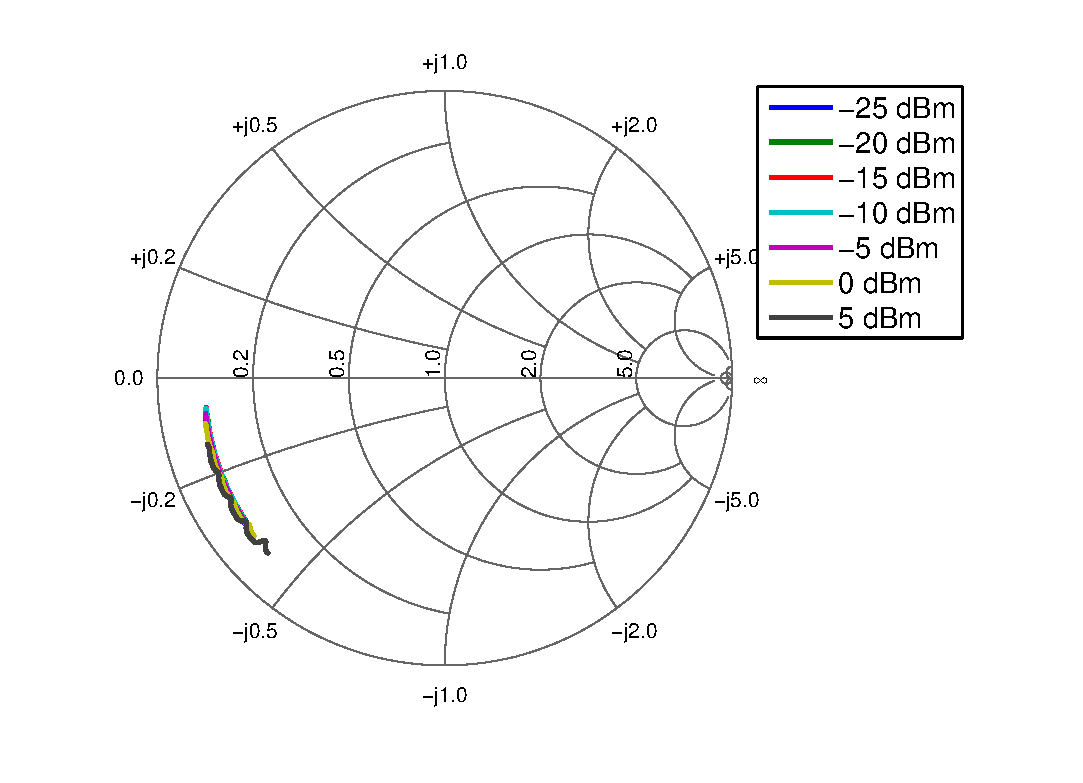
\includegraphics[width=0.45\textwidth]{Pictures/25Feb2013/chip1_saline_impedance}
		\label{fig:chip1_saline_impedance}
		}
		\quad
	\subfigure[Impedance of chip \#2 in saline swept over power]{
		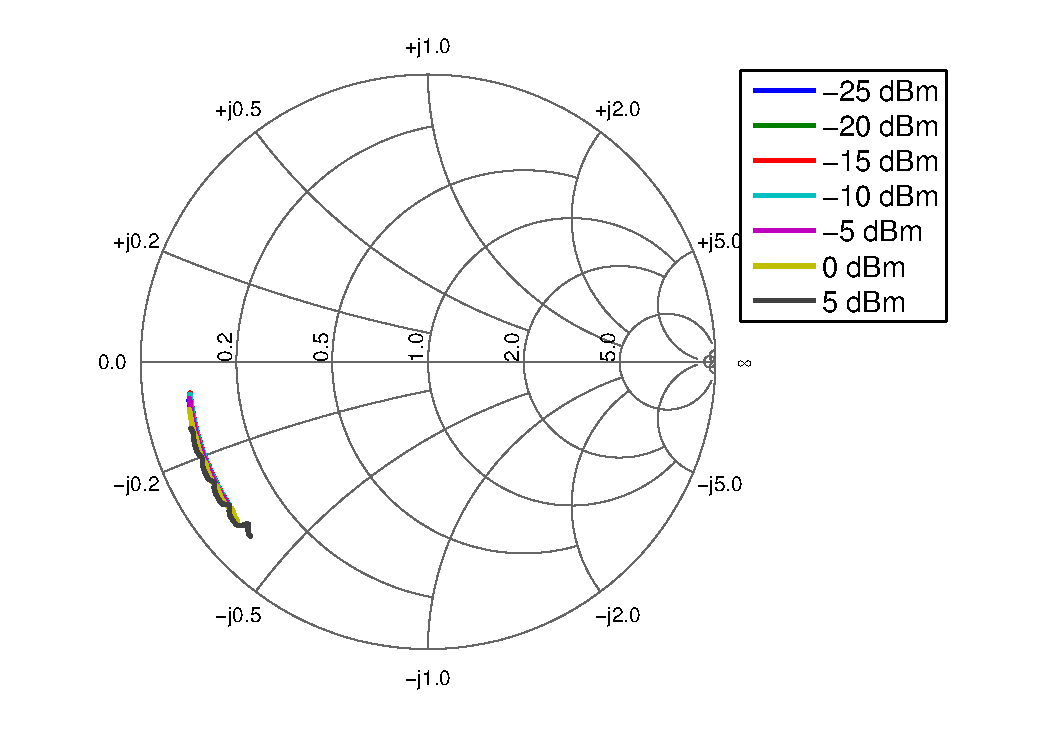
\includegraphics[width=0.45\textwidth]{Pictures/25Feb2013/chip2_saline_impedance} 
		\label{fig:chip2_saline_impedance}
		}
	\label{fig:chip_saline_impedance}
	\caption{Impedance of Bug3 chip in saline. Power swept from -25 dBm to +5 dBm, frequency from 800 MHz - 1 GHz}
\end{figure}

It's pretty clear that these figures are quite similar to Figures \ref{fig:chip1_FS_impedance} and \ref{fig:chip2_FS_impedance}, the impedance of the chip in free space. Not surprisingly, placing the chip in the tank of saline has very little effect on its impedance, as the chip itself is a closed package. Picking out the desired carrier frequency of 915 MHz, we arrive at the reflection coefficients and impedances in Table \ref{tab:chip_saline_impedance}.


%Bug3 chip impedance in saline
\begin{table}[h]
\centering
	\caption{Bug3 chip impedance at 915 MHz in saline}
	\begin{tabular}{| c | c | c | c | c |}
	\hline
	& \multicolumn{2}{|c|}{Chip \#1} & \multicolumn{2}{|c|}{Chip \#2} \\ \hline
	 Power (dBm) & Real/Imag & $R+jX \, \Omega$ & Real/Imag & $R+jX \, \Omega$ \\ \hline
	 -25 &  $-0.7946-j0.2960$ & $4.247-j8.948 \, \Omega$ & $-0.7925-j0.2981$ & $4.287-j9.027 \, \Omega$ \\ \hline
	 -20 & $-0.7970-j0.2696$ & $4.424-j8.164 \, \Omega$ & $-0.7953-j0.2733$ & $4.438-j8.287 \, \Omega$ \\ \hline
	 -15 & $-0.7978-j0.2706$ & $4.393-8.187 \, \Omega$ & $-0.7952-j0.2742$ & $4.434-j8.313 \, \Omega$ \\ \hline
	 -10 & $-0.7975-j0.2732$ & $4.377-8.264 \, \Omega$ & $-0.7946-j0.2763$ & $4.432-j8.380 \, \Omega$\\ \hline
	 -5 & $-0.7957-j0.2918$ & $4.256-8.818 \, \Omega$ & $-0.7933-j0.2935$ & $4.308-j8.889 \, \Omega$  \\ \hline
	 0 & $-0.7870-j0.3299$ & $4.117-j9.990 \, \Omega$ & $-0.7853-j0.3346$ & $4.114-j10.141 \, \Omega$ \\ \hline
	 5 & $-0.7630-j0.4082$ & $3.835-j12.464 \, \Omega$ & $-0.7623-j0.4085$ & $3.850-j12.483 \, \Omega$ \\ \hline
	\end{tabular}
\label{tab:chip_saline_impedance}
\end{table}


Comparing the values in Table \ref{tab:chip_saline_impedance} to those in Table \ref{tab:chip_FS_impedance} further confirms that there is very little difference between the impedance of Bug3 chip in free space and in saline.

Now, we can use the impedance information about the Bug3 chip in saline and the small loop antenna in saline to match the chip impedance to the conjugate of the small loop at 915 MHz.


\subsection{Matching the Bug3 Chip to the Small Loop Antenna in Saline}
\indent \indent The goal here is to match the impedance of the Bug3 chip to the conjugate of the antenna, as this allows for maximum power transfer from the antenna to the chip, although this is not reflection-less. In this instance, it is desired to deliver the most power possible to the chip to allow for maximum operating distance at the cost of some internal reflections.

Thus, since the impedance of the small loop antenna at 915 MHz in the saline is $Z_{{\rm{loop}}}=62.86-j24.38$, we must have:

\[Z_{{\rm{chip}}}=Z_{{\rm{loop}}}^{*}=62.86+j24.38 \]

This is accomplished through a matching network, where the matching point is as above, the conjugate of the small loop antenna in the saline.



%February 26, 2013-----------------------------------------------------------------------------------------------------------------------------------------
\clearpage
\section{26 February 2013:}

\indent \indent Continuing to match the chip to the conjugate of the small loop antenna impedance. 

\subsection{Matching the Bug3 Chip to the Small Loop Antenna in Saline}
\indent \indent Using the impedance matching network designer, a 2-element matching network was designed that would, in the ideal case, transform the impedance seen looking into the chip to that of the conjugate of the small loop antenna while in saline. Using this network designer provides a starting point to perform matching, as there are parasitics that make this ``ideal" network not work as expected.

Altering the ideal network, we arrive at the matching network shown in Figure \ref{fig:Chip1_MN1_saline_schematic} with the impedance on the Smith chart in Figure \ref{fig:Chip1_MN1_saline_smith}.


\begin{figure}[htbp]
	\centering
	\subfigure[Matching network for chip \#1 in saline to match to small loop antenna conjugate]{
		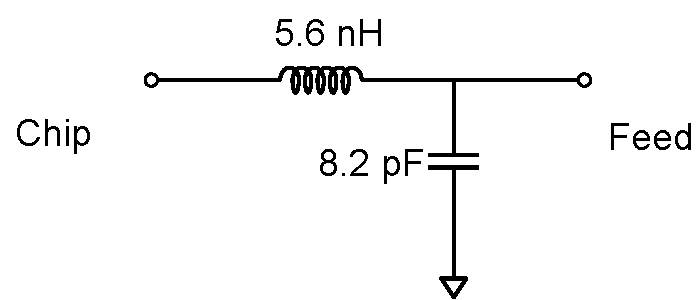
\includegraphics[width=0.45\textwidth]{Pictures/26Feb2013/Chip1_MN1_saline}
		\label{fig:Chip1_MN1_saline_schematic}
		}
		\quad
	\subfigure[Impedance looking into chip from feed point with matching network]{
		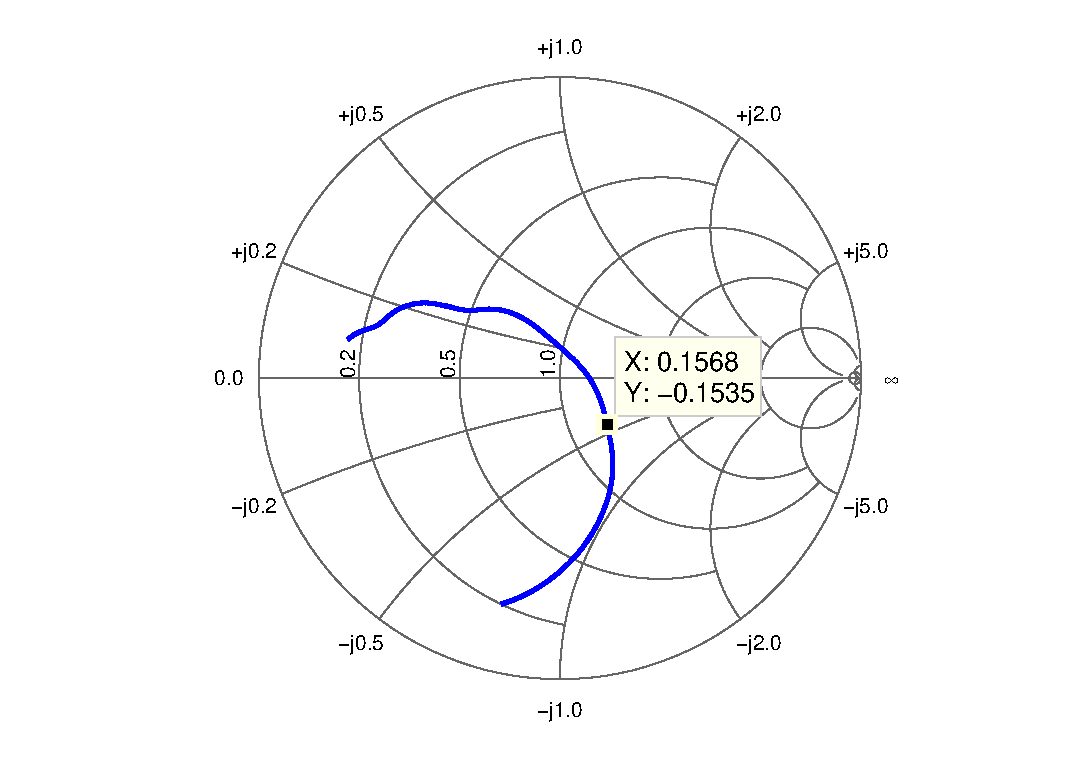
\includegraphics[width=0.45\textwidth]{Pictures/26Feb2013/Chip1_MN1_saline_smith} 
		\label{fig:Chip1_MN1_saline_smith}
		}
	\label{fig:Chip1_MN1_saline}
	\caption{First attempt at matching chip \#1 to conjugate of small loop antenna}
\end{figure}

Marked on the smith chart is the reflection coefficient at 915 MHz. We are trying to match to the conjugate of the small loop antenna's impedance, so we need the impedance seen looking into the chip to be close to $\Gamma = 0.153 + j0.183$, or $Z = 62.86 + j24.38$. Using the matching network in Figure \ref{fig:Chip1_MN1_saline_schematic}, we arrive at:

\[ \Gamma = 0.157 - j0.154 \]

Or

\[Z = 64.80 - j20.89 \]

The impedance achieved through this matching network is quite close to the actual impedance of the small loop antenna at 915 MHz as opposed to its conjugate. This would allow for minimum reflections, but not maximum power transfer. It appears that less capacitance is needed, so utilizing a smaller shunt capacitor might be helpful?

Swapping out the 8.2 pF shunt capacitor for a 6.8 pF capacitor, as shown in Figure \ref{fig:Chip1_MN2_saline_schematic} produces the impedance as shown in Figure \ref{fig:Chip1_MN2_saline_smith}.


\begin{figure}[htbp]
	\centering
	\subfigure[Alternate matching network for chip \#1 in saline to match to small loop antenna conjugate]{
		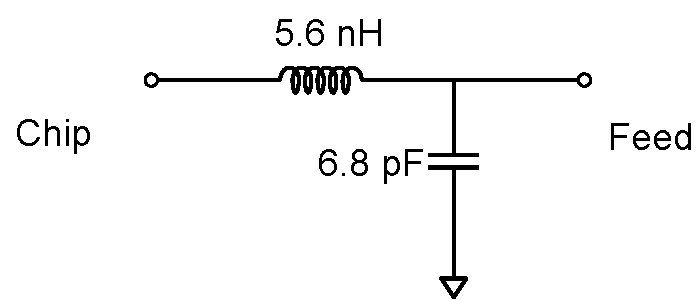
\includegraphics[width=0.45\textwidth]{Pictures/26Feb2013/Chip1_MN2_saline}
		\label{fig:Chip1_MN2_saline_schematic}
		}
		\quad
	\subfigure[Impedance looking into chip from feed point with alternate matching network]{
		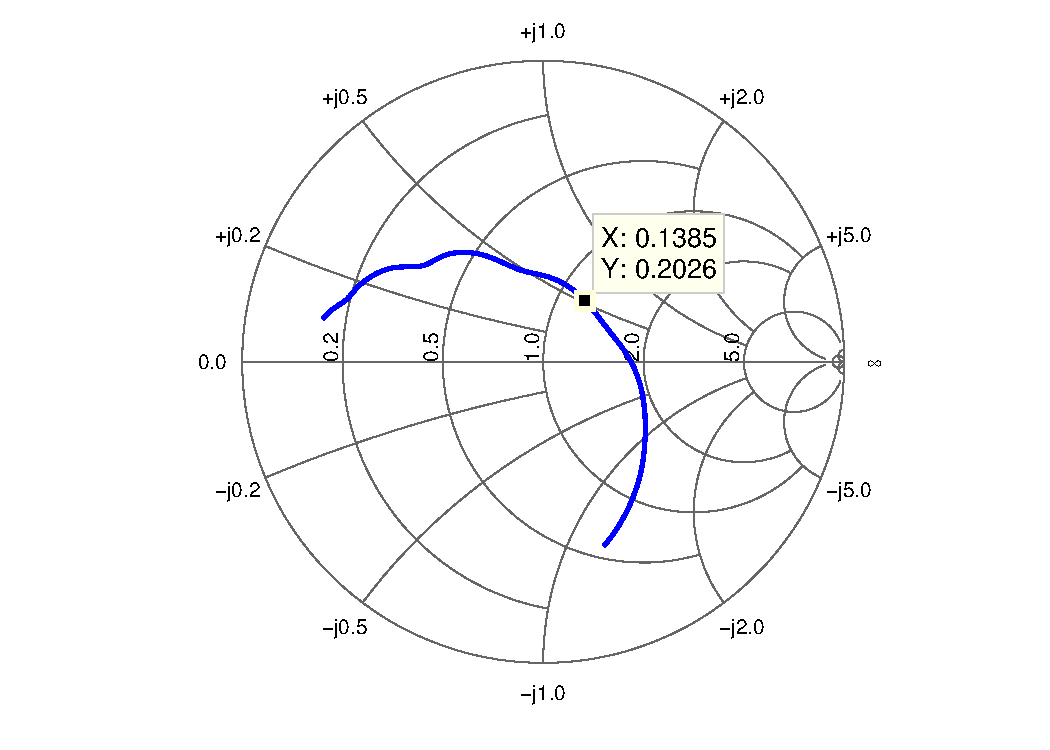
\includegraphics[width=0.45\textwidth]{Pictures/26Feb2013/Chip1_MN2_saline_smith} 
		\label{fig:Chip1_MN2_saline_smith}
		}
	\label{fig:Chip1_MN2_saline}
	\caption{Second attempt at matching chip \#1 to conjugate of small loop antenna}
\end{figure}


Marked on the smith chart in Figure \ref{fig:Chip1_MN2_saline_smith} is the reflection coefficient at 915 MHz. Table \ref{tab:chip1_loop_saline_comparison} shows a comparison between the chip impedance with a matching network in place and the impedance of the small loop antenna.


%Comparison between loop and chip impedance in saline at 915 MHz
\begin{table}[h]
\centering
	\caption{Impedance Characteristics of Single-turn 9.5 mm Diameter Loop in Saline at 915 MHz}
	\begin{tabular}{| c || c | c |}
	\hline
	& Loop & Chip \#1 \\ \hline
	$\Gamma_L$ & $0.153-j0.183$ & $0.139+j0.203$ \\ \hline
	$Z_L$ & $62.86-j24.38 \, \Omega$ & $59.99+j25.87 \, \Omega$ \\ \hline
	\end{tabular}
\label{tab:chip1_loop_saline_comparison}
\end{table}


We can see that the matching network transforms the impedance seen looking into the chip quite close to the conjugate of the small loop's impedance at 915 MHz. To quantify how close we are, we can use the error vector magnitude (EVM). So, if we compare where the matching network brings the chip's impedance to the conjugate of the loop's impedance at 915 MHz, we have the ``ideal" reflection coefficient of:

\[ \Gamma_{{\rm{ideal}}} = 0.153 + j0.183 \]

With the measured reflection coefficient as reported in Table \ref{tab:chip1_loop_saline_comparison}, the error vector magnitude between these two points is as follows:

\[ EVM = 0.0244 \]

Thus, the matching network here will provide a good conjugate match between the chip and single turn small loop antenna in the saline, providing maximum power transfer between the two.


%February 27, 2013-----------------------------------------------------------------------------------------------------------------------------------------
\clearpage
\section{27 February 2013:}

\indent \indent Need to fill this out...data from groupmeeting slide...testing new chip but had to abandon due to unknown error with Vreg...


%February 28, 2013-----------------------------------------------------------------------------------------------------------------------------------------
\clearpage
\section{28 February 2013:}

\indent \indent Trying to finish everything needed for MTT paper, data-wise. Came up with a plan with Matt on the few experiments left to run, as shown below.

\subsection{MTT Paper Completion Plan}

\begin{enumerate}
\item Pass signal (sine wave, ECG data, stored neural data) through chip in chicken and demodulate
\item Impedance characteristics of small single turn 9.5 mm diameter loop in chicken (using VNA)
\end{enumerate}


\subsection{Impedance Characteristics of 9.5 mm Single Turn Loop Antenna in Chicken}
\indent \indent Determining the impedance characteristics of the single turn 9.5 mm diameter loop antenna used on the biotelemetry boards. The antenna ``cal kit" was used to store calibration data and correct subsequent measurements. Measurements were performed in chicken and in free space, as a free space characterization has not been performed yet.

\subsubsection{Free Space}
\indent \indent Calibrating and measuring the antenna's return loss and impedance characteristics in free space. Figures \ref{fig:sngl_loop_FS_smith} and \ref{fig:sngl_loop_FS_RL} show the impedance of the small loop in free space.

\begin{figure}[htbp]
	\centering
	\subfigure[Impedance of single turn loop]{
		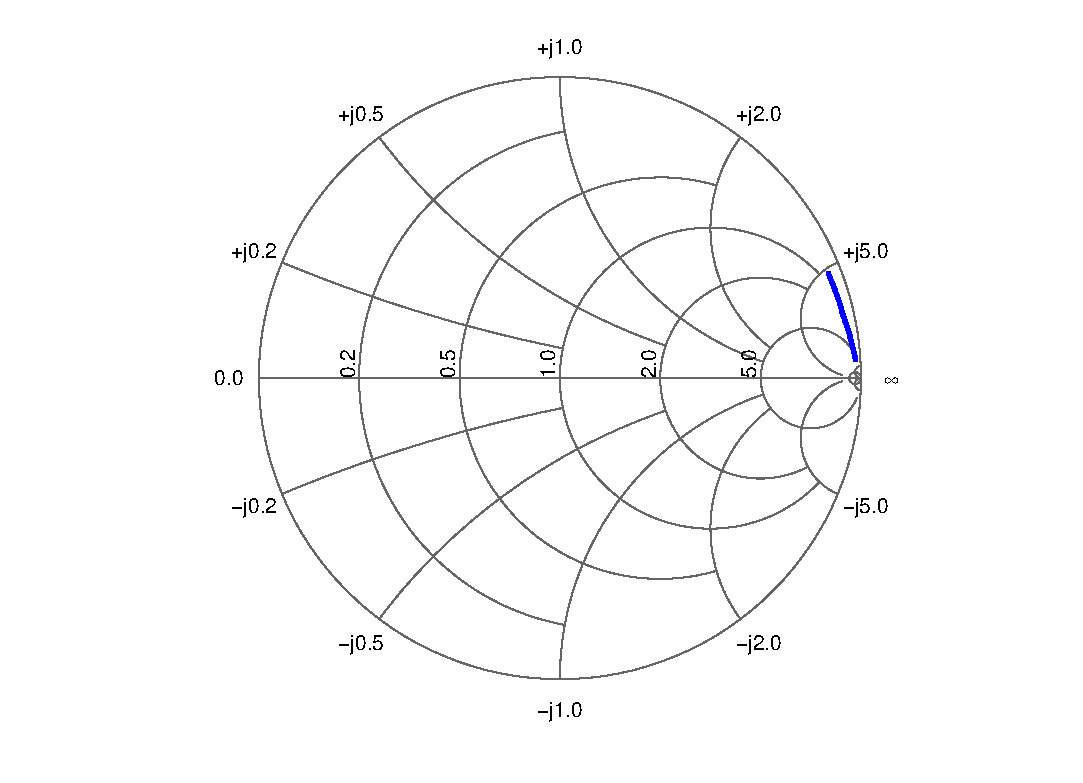
\includegraphics[width=0.45\textwidth]{Pictures/28Feb2013/sngl_loop_FS_smith}
		\label{fig:sngl_loop_FS_smith}
		}
		\quad
	\subfigure[Return loss of single turn loop]{
		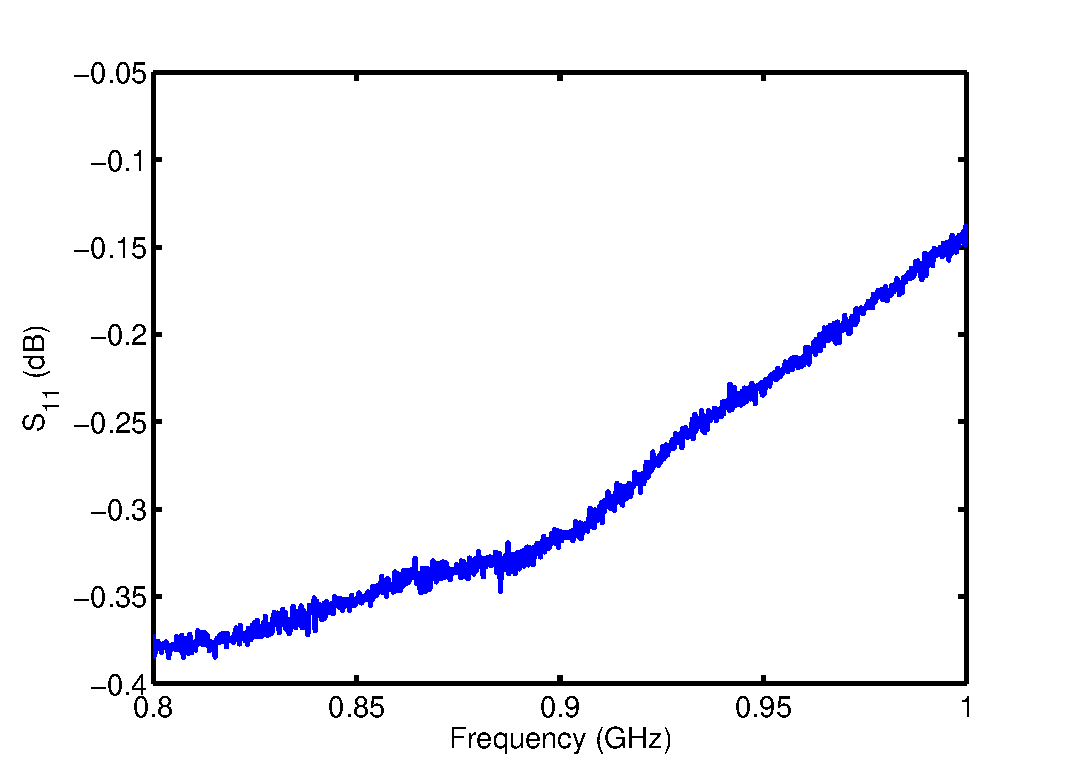
\includegraphics[width=0.45\textwidth]{Pictures/28Feb2013/sngl_loop_FS_RL} 
		\label{fig:sngl_loop_FS_RL}
		}
	\label{fig:sngle_loop_FS}
	\caption{Impedance characteristics of single turn 9.5 mm diameter loop antenna in free space, frequency swept from 800 MHz - 1 GHz}
\end{figure}


The small loop in free space is quite poorly matched to $50 \, \Omega$, as evidenced by its location on the smith chart and its return loss, which is essentially 0 dB, meaning that almost the entire signal being sent into the loop is reflected back. This is not surprising, as small loop antennas are often poor radiators. 

Table \ref{tab:sngl_loop_FS} shows the impedance characteristics at 915 MHz. This reveals how far out on the edge of the smith chart this loop actually is. The magnitude of the reflection coefficient is $|\Gamma_L| = 0.9665$, meaning that almost all of the signal is reflected back. The return loss, as expected, is quite poor, and the loop has a large resistance and reactance. It is very inductive in free space, with an equivalent inductance of 89.62 nH. Due to the loop's impedance being so far out on the edge of the smith chart in free space, it would be quite difficult to match to $50 \, \Omega$, which I ran into previously. 


%Single 9.5 mm diameter loop impedance in free space at 915 MHz
\begin{table}[h]
\centering
	\caption{Impedance Characteristics of Single-turn 9.5 mm Diameter Loop in Free Space at 915 MHz}
	\begin{tabular}{| c || c |}
	\hline
	$\Gamma_L$ & $0.9496+j0.1800$ \\ \hline
	$S_{11}$ & -0.2961 dB \\ \hline
	$Z_L$ & $94.347 + j515.21 \, \Omega$ \\ \hline
	\end{tabular}
\label{tab:sngl_loop_FS}
\end{table}


\subsubsection{Chicken}
\indent \indent Using pieces of skinless, boneless chicken breast as a proxy for muscle/human tissue, the impedance of the small single turn loop was investigated in this scenario. The ``cal kit" was again used to store the calibration data in this new media. Figures \ref{fig:sngl_loop_chicken_smith} and \ref{fig:sngl_loop_chicken_RL} show the results.


\begin{figure}[htbp]
	\centering
	\subfigure[Impedance of single turn loop in chicken]{
		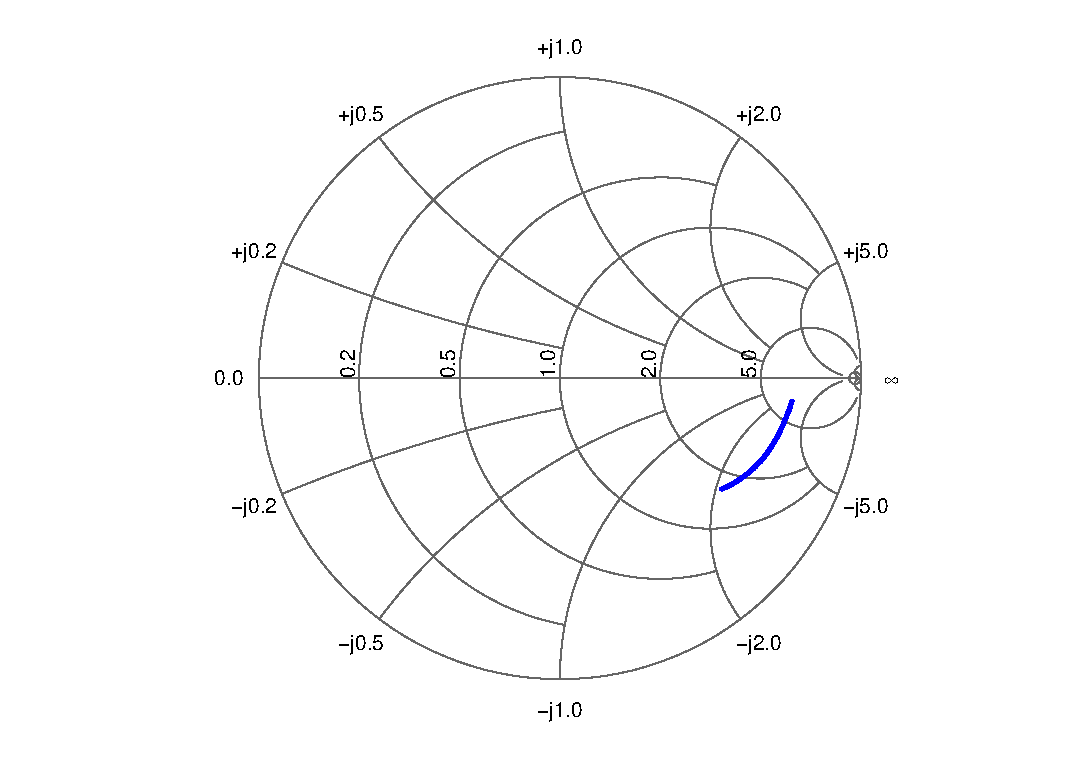
\includegraphics[width=0.45\textwidth]{Pictures/28Feb2013/sngl_loop_chicken_smith}
		\label{fig:sngl_loop_chicken_smith}
		}
		\quad
	\subfigure[Return loss of single turn loop in chicken]{
		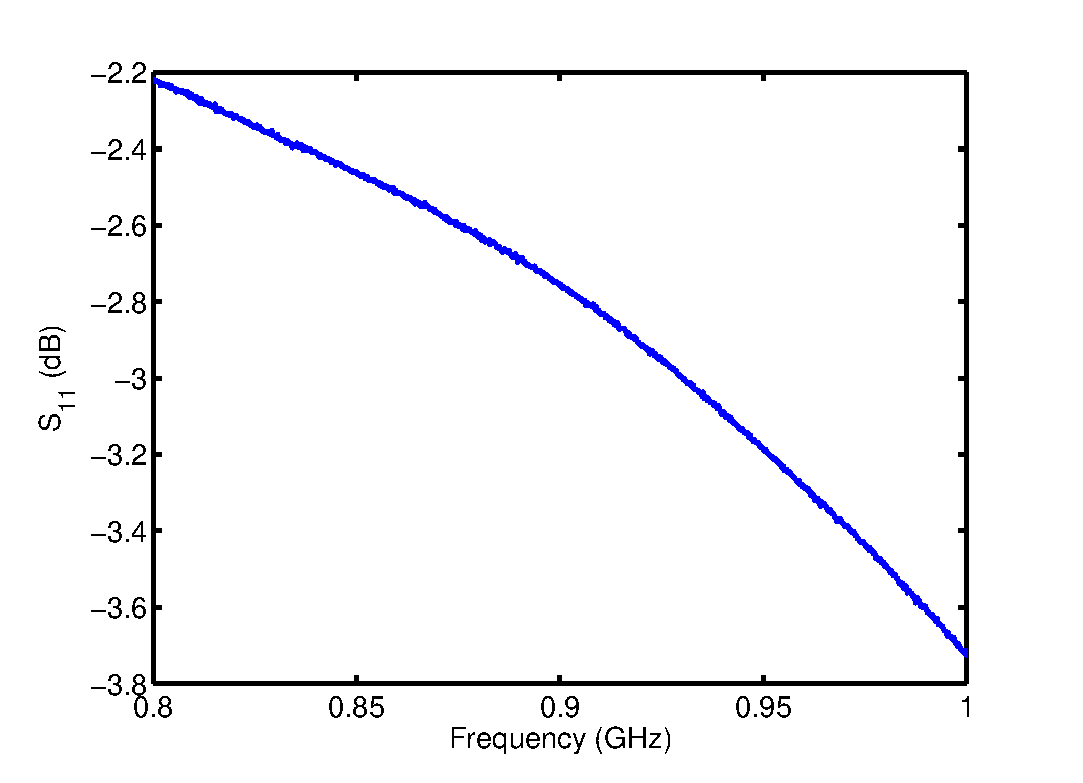
\includegraphics[width=0.45\textwidth]{Pictures/28Feb2013/sngl_loop_chicken_RL} 
		\label{fig:sngl_loop_chicken_RL}
		}
	\label{fig:sngle_loop_chicken}
	\caption{Impedance characteristics of single turn 9.5 mm diameter loop antenna in chicken, frequency swept from 800 MHz - 1 GHz}
\end{figure}

The small loop in chicken is more closely matched to $50 \, \Omega$ than it is in free space, but not as close as it is in saline. Table \ref{tab:sngl_loop_chicken} shows the loop's impedance characteristics at 915 MHz.


%Single 9.5 mm diameter loop impedance in chicken at 915 MHz
\begin{table}[h]
\centering
	\caption{Impedance Characteristics of Single-turn 9.5 mm Diameter Loop in Chicken at 915 MHz}
	\begin{tabular}{| c || c |}
	\hline
	$\Gamma_L$ & $0.6615-j0.2806$ \\ \hline
	$S_{11}$ & -2.8707 dB \\ \hline
	$Z_L$ & $125.08-j145.15 \, \Omega$ \\ \hline
	\end{tabular}
\label{tab:sngl_loop_chicken}
\end{table}


The loop is more closely matched to $50 \, \Omega$ than in free space, with a return loss that is about 2.5 dB better at 915 MHz. It still has a large reactive component and an even larger resistive component, with an equivalent inductance of 25.25 nH.

The main reason for investigating this, besides being useful for the MTT paper, is to see how the matching between the chip and loop antenna will perform when moved from the saline medium to chicken. The matching network was designed with saline in mind, so the chip is matched to the loop's conjugate when in the saline. 


%March 1, 2013-----------------------------------------------------------------------------------------------------------------------------------------
\clearpage
\section{1 March 2013:}

\indent \indent Yesterday, I tried to inject a signal into the chip, and demodulate it through a piece of chicken. While the chicken should be theoretically less lossy than the saline, it was difficult to cleanly demodulate the signal coming through the chip. Even when the chip was fully powered with 4-5 V, the signal being demodulated was very noisy, and the receiver software had a difficult time latching on.

\subsection{Chip Mismatch in Chicken}
The experiment that was conducted used a piece of chicken folded on top of itself, with the device in the middle so that there was chicken surrounding the implant loop. I felt this represented a practical implant situation. There was about 1-1.5 cm of chicken on each side of the implant loop. It appeared that once the upper half of the chicken on the backside of the implant loop was lifted and moved away from the loop, the demodulated signal became much cleaner. This points to the fact that the issue here is probably due to antenna tuning. This is not surprising, as the antenna has been matched to the chip for implantation in the saline, and as we can see from the data the other day, the loop's impedance characteristics are much different when ``implanted" in the chicken.

In fact, we can look more closely at how the matching is affecting the loop's performance in the saline. In the saline, the loop's impedance is: $Z_{{\rm{saline}}} = 62.86 - j24.38$, so we matched the chip to $62.86 + j24.38$. In the chicken, the loop's impedance is: $Z_{{\rm{chicken}}} = 125.08 - j145.15$, so the chip should be matched to $125.08 + j145.15$ for maximum power transfer. If we look at the magnitude of the reflection coefficient between the current matching point of the chip and what it should be in the chicken, we can get an idea of what we're losing due to matching in the chicken. 

\[|\Gamma_{{\rm{mismatch}}}| = 0.537 \]

This indicates that we lose about half the signal strength due to the mismatch between the antenna and chip in the chicken, which could explain why it was so difficult to demodulate a clean signal in the chicken, even at relatively close depths where enough voltage was being harvested. 

\subsection{Demodulating a Signal in Saline}
\indent \indent Since the chip is matched to the loop in saline, we should be able to inject a signal through the chip and demodulate it. After some quick preliminary tests, it looks as though we can demodulate a signal with the device in saline at implantation depths of up to 1.5 cm. As per the plan from yesterday, I'm going to try out injecting a few sine waves of varying frequency, some ``ideal" ECG data from the function generator, and possibly some pre-recorded neural data.

\subsubsection{Sine Wave Demodulation}
\indent \indent Using the original device in the tank of saline and placing it at a distance of 1.5 cm, a sine wave was injected into neural input 1 (N1). The sine wave was 500 Hz, and was set to a peak-to-peak voltage of 10 mV. However, since the device is essentially looking for signals that are in the $\mu V$ range, a 3 dB attenuator was added. The resulting demodulated signal can be seen in Figures \ref{fig:sine500Hz_1p5cm_saline_demod_filt} and \ref{fig:sine500Hz_1p5cm_saline_demod_compare}.


\begin{figure}[htbp]
	\centering
	\subfigure[Received \& demodulated sine wave, using different filtering techniques]{
		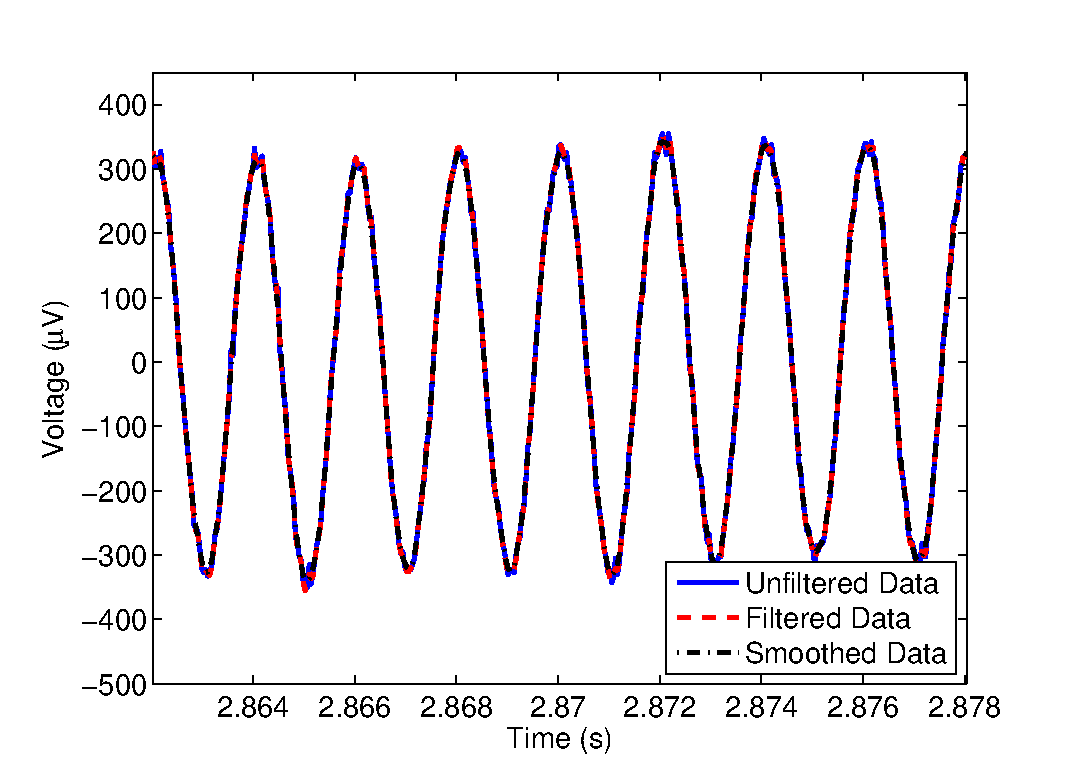
\includegraphics[width=0.45\textwidth]{Pictures/1Mar2013/sine500Hz_1p5cm_saline_demod_filt}
		\label{fig:sine500Hz_1p5cm_saline_demod_filt}
		}
		\quad
	\subfigure[Received, demodulated and filtered signal vs. the original]{
		\includegraphics[width=0.45\textwidth]{Pictures/1Mar2013/sine500Hz_1p5cm_saline_demod_compare} 
		\label{fig:sine500Hz_1p5cm_saline_demod_compare}
		}
	\label{fig:sine500Hz_1p5cm_saline_demod}
	\caption{Injecting a sine wave into the device and demodulating the output. The device is in saline, and 1.5 cm away from the Tx antenna}
\end{figure}

Since the signal being injected is an ideal sine wave, I just reproduced a sine wave of the same frequency in Matlab, and shifted it until it lined up well with the demodulated data. Here, the original data created in Matlab is not the same amplitude as the data injected into the device, just to show how well they line up. The actual amplitude of the original data was 10 mV peak-to-peak, but was passed through a 3 dB attenuator before being injected into the device, as it is searching for signals on the order of $\mu V$.


%March 4, 2013-----------------------------------------------------------------------------------------------------------------------------------------
\clearpage
\section{4 March 2013:}

\indent \indent On Friday, signals were injected into the device in the tank of saline and successfully demodulated using the current receiver setup. A few sine waves of varying frequency, as well as some ideal cardiac data was sent through the device. A couple of plots of this data are shown from Friday, and here we'll plot the rest. Also, the figures in the current version of the MTT paper will be modified and polished until they're ready to go. After that, the text will be fixed/finished.

\subsection{Demodulating a Signal in Saline}
\indent \indent Here are the results of injecting a signal into the device in saline and demodulating the data and comparing it with the original. Some post-processing was used to clean up the demodulated data.

\subsubsection{Demodulating a Sine Wave in Saline}
\indent \indent The results shown in Figures \ref{fig:sine250Hz_1p5cm_saline_demod_compare}, \ref{fig:sine500Hz_1p5cm_saline_demod_compare} and \ref{fig:sine750Hz_1p5cm_saline_demod_compare} show the demodulated sine wave versus the original over a few different input sine wave frequencies. 


\begin{figure}[htbp]
	\centering
	\subfigure[250 Hz sine wave]{
		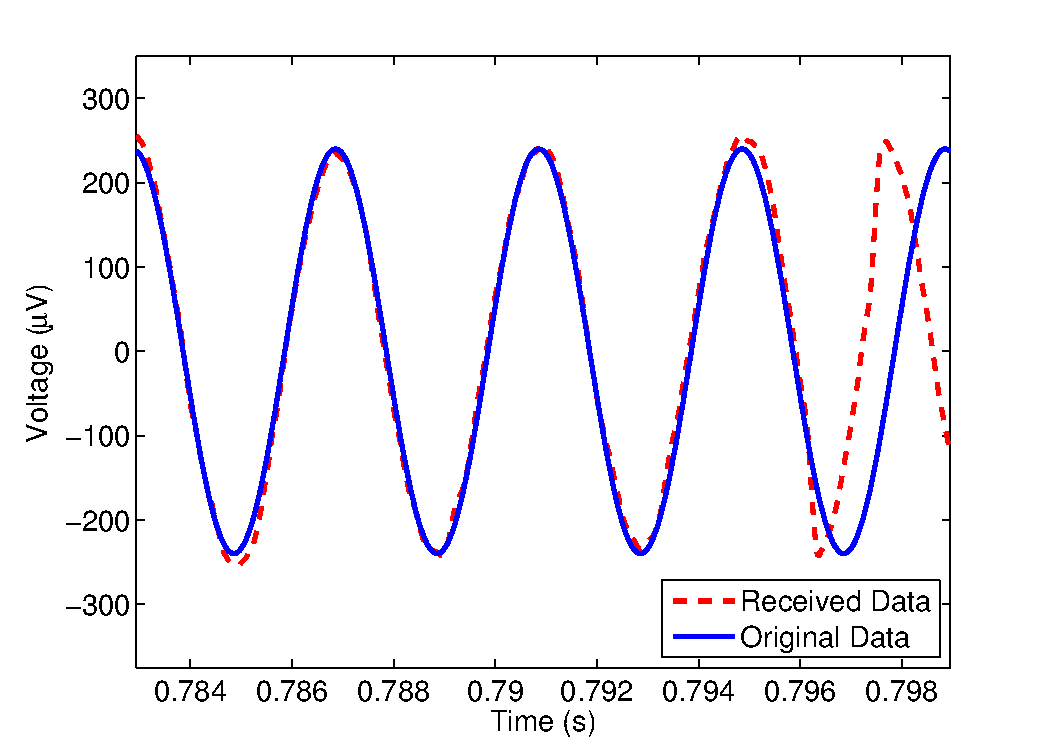
\includegraphics[width=0.45\textwidth]{Pictures/4Mar2013/sine250Hz_1p5cm_saline_demod_compare}
		\label{fig:sine250Hz_1p5cm_saline_demod_compare}
		}
		\quad
	\subfigure[500 Hz sine wave]{
		\includegraphics[width=0.45\textwidth]{Pictures/4Mar2013/sine500Hz_1p5cm_saline_demod_compare} 
		\label{fig:sine500Hz_1p5cm_saline_demod_compare}
		}
		\quad
	\subfigure[750 Hz sine wave]{
	\includegraphics[width=0.45\textwidth]{Pictures/4Mar2013/sine750Hz_1p5cm_saline_demod_compare}
	\label{fig:sine750Hz_1p5cm_saline_demod_compare}
	}
	\label{fig:sine_1p5cm_saline_demod_compare}
	\caption{Injecting a sine wave into the device and demodulating the output. The device is in saline, and 1.5 cm away from the Tx antenna. Sine waves of 250 Hz, 500 Hz and 750 Hz are shown}
\end{figure}


The demodulated data output has been post-processed in Matlab using lowpass filters to clean up the signal. The original data has also been scaled down for comparison. We can see that for 500 Hz and 750 Hz input sine waves, the demodulated output resembles the original input data quite accurately and appears to be of the same frequency. The 250 Hz input sine wave matches well for most of the cycles seen, but deviates by a few Hz during the last shown cycle. This can be explained by the frequency response of the biopotential amplifiers present on the Bug3 chip, as this is close to their lower frequency in their 3 dB bandwidth. Their 3 dB bandwidth is approximately 200 Hz - 13 kHz (measured by Stewart) and 250 Hz - 13 kHz simulated (from Reid Harrison). 

The input signals were generated from an signal generator, and the input peak-to-peak voltage was set at 10 mV. However, since the chip is looking for signals in the $\mu V$ range, a 30 dB attenuator was added between the signal generator and the chip's 1st neural amplifier input. In any case, it is clear that we are able to accurately demodulate a signal passing through the device while it is completely passively powered at a distance of 1.5 cm away in a tank of saline, using a small octagonal segmented loop as the transceiving antenna.

A good match between transmitted and demodulated data is seen for a zoomed-in section of the data for each frequency tested. However, during the last shown cycle of the 250 Hz sinusoid, we can see that there is a significant deviation between the original, transmitted signal, and the demodulated signal at the receiver. This is probably due to the frequency response of the neural amplifiers, as 250 Hz is on the edge of their 3-dB bandwidth, so section of the transmitted signal may have been attenuated a great deal, making it difficult for the receiver to accurately determine the backscattered signal.


\subsubsection{Demodulating ECG Data in Saline}
\indent \indent In addition to the sine waves used to test out demodulating a signal using the ``implanted" device, ideal ECG data was also used. This is a proxy for biological information, and will show that we can demodulate biological information accurately at a decent implant depth. 

See tomorrow for more details on this...



%March 5, 2013-----------------------------------------------------------------------------------------------------------------------
\clearpage
\section{5 March 2013:}

\indent \indent Here, processing the demodulated ECG data in the saline tank was worked on. At first, I thought using the {\bf{ecg.m}} file in Matlab to produce ``ideal" ECG data for the transmitted data would work out fine. But, I found out that the file accepts an argument which represents the length of the signal, and then it produces a single ``blip" of an ECG signal with all the correct features. You can't choose how far apart the features are, and setting a ``heart rate" would be a bit tricky since we have control over so little.

So, instead of using this function to produce the transmitted data to compare the demodulated data to, we simply connected the function generator to the oscilloscope and captured exactly what was routed to the chip. This trace data was saved and imported into Matlab for plotting.

Below are the results of looking at the comparison between the transmitted and demodulated ECG data.

\subsection{Demodulating ECG Data in Saline}
\indent \indent First, I took a look at the raw demodulated data, and then tried a couple of different filtering techniques. Normally, for ECG data, it is passed through a bandpass filter from 0.05 - 40 Hz. However, this won't work here since we have a repetition rate of 750 Hz, and this will cut off all the high frequency information. The frequency that the function generator was set to determines the ``heart rate," the distance between features of the ECG data. A bandpass filter from 0.05 - 1700 Hz was tried instead. Also, a smoothing filter was used separately to see if it could perform better than the bandpass filter. A Savitzky-Golay filter of degree 2 and a frame of 5 was used. Finally, using the exact transmitted ECG data at 750 Hz as described above, it was downsampled to match the sampling frequency of the neural inputs on the chip (250 MHz scope vs. 26.1 kHz on chip). The results are shown in the figure below.



\begin{figure}[htbp]
	\centering
	\subfigure[Raw demodulated data and filtering techniques]{
		\includegraphics[width=0.45\textwidth]{Pictures/5Mar2013/ecg750Hz_demod_saline_filt_compare}
		\label{fig:ecg750Hz_demod_saline_filt_compare}
		}
		\quad
	\subfigure[Transmitted data vs. raw demodulated data]{
		\includegraphics[width=0.45\textwidth]{Pictures/5Mar2013/ecg750Hz_demod_compare} 
		\label{fig:ecg750Hz_demod_compare}
		}
		\quad
	\subfigure[Transmitted data vs. filtered demodulated data]{
	\includegraphics[width=0.45\textwidth]{Pictures/5Mar2013/ecg750Hz_filt_demod_compare}
	\label{fig:ecg750Hz_filt_demod_compare}
		}
		\quad
	\subfigure[Transmitted data vs. smoothed demodulated data]{
	\includegraphics[width=0.45\textwidth]{Pictures/5Mar2013/ecg750Hz_smooth_demod_compare}
	\label{fig:ecg750Hz_smooth_demod_compare}
		}
	\label{fig:ecg750Hz_demod}
	\caption{Injecting an ECG signal into the device and demodulating the output. The device is in saline, and 1.5 cm away from the Tx antenna. Results using a 750 Hz ideal ECG signal are shown.}
\end{figure}

It's late...too tired to explain these right now...but need them for MTT paper and slides tomorrow. Include a couple of the above figures along with the sine wave demodulation. Include a line drawing too? Can use the unfinished one...should be in MTT figure sources folder...



%March 6, 2013-----------------------------------------------------------------------------------------------------------------------
\clearpage
\section{6 March 2013:}

\indent \indent Looking at the plots of the demodulated sine wave and ECG data versus the original transmitted data, the scaling of the original data was off previously. I was just choosing a scale for the original data to make a comparison easy, but now I'ver figured out the actual amplitude of the transmitted data.

We have a 10 mV peak-to-peak signal passing through a 30 dB attenuator, so this should be a {\bf{voltage}} gain of $\frac{1}{31.62}$. This brings us to 10 mV x $\frac{1}{31.62}$, or $316.3 \mu$V. Now, since the amplifier input on the chip is not $50 \, \Omega$, this value essentially doubles, so we have a peak-to-peak voltage at the chip of: $632.5 \mu$V.

Using this new information, the plots of the sine wave and ECG data can be fixed up a bit. Also, there might be a slight DC offset in the demodulated data, so removing this offset and re-centering the data around 0 should help, especially with the ECG data. One other thing to check could be the frequency content of the ECG data, since the high frequency spikes might be outside the amplifier's frequency response. Figures \ref{fig:sine250Hz_1p5cm_saline_demod_compare}, \ref{fig:sine500Hz_1p5cm_saline_demod_compare} and \ref{fig:sine750Hz_1p5cm_saline_demod_compare} show the results. 

\begin{figure}[htbp]
	\centering
	\subfigure[250 Hz sine wave]{
		\includegraphics[width=0.45\textwidth]{Pictures/6Mar2013/sine250Hz_1p5cm_saline_demod_compare}
		\label{fig:sine250Hz_1p5cm_saline_demod_compare}
		}
		\quad
	\subfigure[500 Hz sine wave]{
		\includegraphics[width=0.45\textwidth]{Pictures/6Mar2013/sine500Hz_1p5cm_saline_demod_compare} 
		\label{fig:sine500Hz_1p5cm_saline_demod_compare}
		}
		\quad
	\subfigure[750 Hz sine wave]{
	\includegraphics[width=0.45\textwidth]{Pictures/6Mar2013/sine750Hz_1p5cm_saline_demod_compare}
	\label{fig:sine750Hz_1p5cm_saline_demod_compare}
		}
	\label{fig:sine_demod_fix}
	\caption{Injecting a sine wave into the device and demodulating the output. The device is in saline, and 1.5 cm away from the Tx antenna. Results have been fixed to show the true amplitude of the Tx and Rx signals.}
\end{figure}


The poor match for the 250 Hz sine wave is more obvious here, as is the good match between the transmitted and received sine wave for the 500 Hz and 750 Hz case. This is due to the frequency response of the neural amplifiers, as their 3 dB bandwidth is approximately 250 Hz - 13 kHz, and the 250 Hz falls on the lower extreme of what they're capable of doing, so the fact that the 250 Hz sine wave does not match well both in amplitude and a slight time shift distortion is not surprising. 


%March 7, 2013-----------------------------------------------------------------------------------------------------------------------
\clearpage
\section{7 March 2013:}

\indent \indent Nothing to show here today...sorry! Working on figures for the MTT paper using data that has already been saved. Mainly fixing up some diagrams, changing some labels, etc. So not much to show here....maybe next time.


%March 8, 2013-----------------------------------------------------------------------------------------------------------------------
\clearpage
\section{8 March 2013:}

\indent \indent Still working on the figures for the MTT paper. Having a difficult time getting the transmitted and received ECG signals to match up well, so letting that one sit for a bit and finishing all the other figures. Will have to come back to the ECG signals before that figure/section can be completed.

\subsection{Demodulating ECG Data in Saline}
\indent \indent Matt had a couple of good suggestions for making this data look alright, since the data shown in Figure \ref{fig:ecg750Hz_smooth_demod_compare} don't show enough of a match to be presentable. Also, the ``ideal" ECG data shows some slight amplitude modulation in the spikes, so this means that the ``ideal" data isn't really ideal, and this needs to be fixed prior to submission.

A couple of ideas to fix this:
\begin{enumerate}
\item Bandlimit the Tx signal to that of the bandwidth of the neural channel's sampling rate - can use BPF with appropriate passband, and then downsample
\item Anti-aliasing of the Rx signal, so it resembles the Tx data
\end{enumerate}

At first, these processing ideas did not seem to work, and the Tx and Rx data were still not very similar. The problem seemed to lie in the filtering of the Tx data. The problem is, the Tx data is sampled at 250 MHz, and we are only concerned with the band 250 Hz - 13 kHz, so creating a decent filter for the Tx data is difficult. This means that the filter order, the number of taps, needs to be quite large. The filter orders I was using at first were too small to properly BPF the Tx data. The filter order needs to be increased to about 100 or greater to properly filter this data. Attempt either a BPF or LPF, but also try to get rid of DC offset from chip.



%March 11, 2013-----------------------------------------------------------------------------------------------------------------------
\clearpage
\section{11 March 2013:}

\indent \indent Worked more on the figures for the MTT paper, as well as the RFID 2013 paper which was conditionally accepted and is now being shepherded. The reviewers have a few points that we need to address, and once that is completed, the paper will be accepted. I've started a document outlining the points we need to address and how we will address them. This is the first deadline in the shepherding process, and needs to be submitted to our shepherd by March 15 (Friday). 



%March 12, 2013-----------------------------------------------------------------------------------------------------------------------
\clearpage
\section{12 March 2013:}

\indent \indent Today I looked at a few points in the RFID 2013 paper shepherding that we can address, including taking a bit more data of an ``ideal" ECG signal being transmitted OTA.

\subsection{RFID 2013 Paper Shepherding}
\indent \indent Addressing a few of the points for the passive ECG paper shepherding.

\subsubsection{Telemetry Device Power Breakdown: Only Used Channels}
\indent \indent One point brought up was the modest range of the system, which we found to be $\approx$ 1 meter. One of the reasons for the modest read distance is the fact that the device is currently setup to sample and transmit all 16 channels, regardless of whether or not there is useful information on those channels, so it is wasting power. For the 3 and 5-lead ECG's, we are only using a small subset of the available channels, and if we could turn off the unused channels, we would conserve power on the chip, and could achieve a greater read distance at the cost of a lower aggregate data rate. In the TBioCAS paper, there was a simulation-based power breakdown of the components on the chip. Using this table, we can determine how much current and power we would save if we only transmitted data from used channels in each ECG setup. Table \ref{tab:IC_pwr_breakdown} shows the results.

Since we know that the harvester and mismatch efficiency is 20.6\% from the TBioCAS paper, we can determine the minimum power up threshold at the terminals of the IC as follows: $P_{{\rm{thresh}}} = 10 \log_{10} \left( \frac{{\rm{IC_{pwr}}}}{0.206} \right)$

%Power breakdown of chip, saved power by only considering used channels
\begin{table*}[h]
\scriptsize
\centering
	\caption{Power breakdown of telemetry IC: Channel subset}
	\begin{tabular}{ l c r| c r| c r|}
	& & & \multicolumn{2}{c}{3-lead ECG} & \multicolumn{2}{c}{5-lead ECG} \\ \hline \hline
	Neural amplifiers & 10 x 16 $\mu$A & 160 $\mu$A & 3 x 16 $\mu$A & 48 $\mu$A & 4 x 16 $\mu$A & 64 $\mu$A \\
	EMG amplifiers & 4 x 0.25 $\mu$A & 1 $\mu$A & 0 x 0.25 $\mu$A & 0 $\mu$A & 0 x 0.25 $\mu$A & 0 $\mu$A \\
	DC amplifiers & 2 x 45 $\mu$A & 90 $\mu$A & 0 x 45 $\mu$A & 0 $\mu$A &  0 x 45 $\mu$A & 0 $\mu$A \\
	Analog mux & & 139 $\mu$A & & 139 $\mu$A & & 139 $\mu$A \\
	Amplifier / mux bias generators & & 80 $\mu$A & & 80 $\mu$A & & 80 $\mu$A \\
	11-bit ADC and digital control logic & & 320 $\mu$A & & 320 $\mu$A & & 320 $\mu$A\\
	LDO voltage regulator & & 60 $\mu$A & & 60 $\mu$A & & 60 $\mu$A \\
	Crystal oscillator & & 70 $\mu$A & & 70 $\mu$A & & 70 $\mu$A \\
	Backscatter modulator & & 15 $\mu$A & & 15 $\mu$A & & 15 $\mu$A \\
	\hline
	{\bf{Simulated}} Total IC supply current & & 935 $\mu$A & & 732 $\mu$A & & 748 $\mu$A \\
	& & & & & & \\
	& & & & & & \\
	Minimum unregulated supply voltage & & 1.31 V & & 1.31 V & & 1.31 V \\
	{\bf{Simulated}} Total IC power consumption & & 1.22 mW & & 0.959 mW & & 0.980 mW \\
	& & & & & & \\
	Power up threshold (for 20.6\% harvester) & & +7.76 dBm & & +6.68 dBm & & +6.77 dBm \\
	\end{tabular}
\label{tab:IC_pwr_breakdown}
\end{table*}

Here, we can clearly see that by only using a subset of the available channels necessary for certain types of ECG, we can save on power consumption of the telemetry device, leading to a reduced power-up threshold at the terminals of the IC. This will in turn have an effect on the effective fully-passive operating distance of the device, which is investigated below.

\subsubsection{Operating Range Only Using Required Channels}
\indent \indent Here, we investigate the maximum operating range of the fully passive telemetry device using the power thresholds calculated in Table \ref{tab:IC_pwr_breakdown}. Using the following equation, we can determine the maximum operating range:

\begin{eqnarray}
P_{thresh} &=& P_{Tx}+G_{Tx}-PL+G_{Rx}  \\
PL &=& P_{Tx}+G_{Tx}+G_{Rx}-P_{thresh} \\
20\log(d_{max})+20\log(f)-27.55 &=& P_{Tx}+G_{Tx}+G_{Rx}-P_{thresh} \\
d_{max} &=& 10^{\frac{P_{Tx}+G_{Tx}+G_{Rx}-P_{thresh}+27.55-20\log(f)}{20}}
\end{eqnarray}

Using this equation and $P_{Tx}=28$ dBm, $G_{Tx}=8$ dBi, $G_{Rx}\approx0$ dBi, and $P_{thresh}$ as the values shown in Table \ref{tab:IC_pwr_breakdown}, we find the following maximum operating distances for different amounts of active channels. The results are shown in Table \ref{tab:max_op_dist}.

%Maximum theoretical range with different power thresholds
\begin{table}[h]
\centering
	\caption{Maximum Theoretical Range For Different Power Thresholds}
	\begin{tabular}{| c | c | c |}
	\hline
	{\bf{Measurement Type}} & $P_{thresh}$ & $d_{max}$ \\ \hline
	All channels & +7.76 dBm & 0.67 m \\ \hline
	3-lead ECG (3 channels) & +6.68 dBm & 0.76 m \\ \hline
	5-lead ECG (4 channels) & +6.77 dBm & 0.75 m \\ \hline
	\end{tabular}
\label{tab:max_op_dist}
\end{table}

We can see that by decreasing the amount of active channels, we lower the power threshold of the IC and increase the operating distance, though only slightly. We can gain about 10 cm of operating distance, theoretically, for a 3-lead or 5-lead ECG setup by turning off unused channels.

\subsubsection{Calculating Semi-passive Ideal Range}
\indent \indent Still discussing the so-called modest range of the telemetry system, some of the reviewers mentioned semi-passive operation. This would increase the range of the system, as the device would not need to receive a certain power level to turn-on, and the most significant contributor to the operating range would be the receiver sensitivity. 

If we assume a 10 dB receiver noise figure, we can determine the theoretical maximum operating range of the device based on theoretical receiver sensitivity. According to the TBioCAS paper, the input referred noise to the receiver is -88 dBm. With the assumed 10 dB noise figure, this leads to a sensitivity of approximately -78 dBm (which seems a bit low...?). In the TBioCAS paper, the NF was 13 dB, and the claimed sensitivity was about -70 dBm, so here, we are going to use a sensitivity of -73 dBm.

In order to determine the maximum range, we are essentially limited by path loss. The equation to determine the maximum range is shown below

\begin{eqnarray}
P_{Rx} =& P_{Tx} - PL + BS_{ratio} - PL + G_{ant} \\
P_{Rx} = & P_{Tx} - 2PL + BS_{ratio} + G_{ant} \\
PL =& \frac{P_{Tx}+BS_{ratio}+G_{ant}-P_{Rx}}{2} \\
20\log(d_{max})+20\log(f)-27.55 =& \frac{36 {\rm{dBm}} - 15 {\rm{dB}} + 8 {\rm{dBi}} - (-73 {\rm{dBm}})}{2} \\ 
\log(d_{max}) =& 0.966 \\
d_{max} =& 9.25 {\rm{m}}
\end{eqnarray}

This theoretical range seems rather large, so I'm not sure if this was done right. If we change the sensitivity to -70 dBm, we find $d_{max} = 7.78$ m, and with a sensitivity of -60 dBm, we find $d_{max}=4.38$ m.


%March 13, 2013-----------------------------------------------------------------------------------------------------------------------
\clearpage
\section{13 March 2013:}

\indent \indent Looking at the OTA test using ``ideal" ECG data for the passive ECG experiment. I re-took this data the other day using both a bistatic and monostatic setup, but it turns out I actually had some of this data previously. I had taken essentially the same dataset in December, when trying to prepare the paper.

One strange thing that is clear from looking at the plots to follow is that for the ideal ECG data at a rep rate of between 1 and 2 Hz, the demodulated data does not resemble the original transmitted data at all. In fact, the demodulated data doesn't even resemble an ECG signal anymore. However, when I took the data with the electrodes connected to myself and viewed the demodulated output, the output waveforms, once they've been cleaned up, resemble ECG signals, and the salient features can be picked out. The ECG signals coming from my body are also at a rep rate of between 1 and 2 Hz, yet they are demodulated just fine, for the most part. Why is it that the ``ideal" ECG data at a similar rep rate fails to be demodulated cleanly and resemble the original transmitted signal?

\subsection{More RFID Shepherding}
\indent \indent More items to address for the shepherding of the RFID paper. 

\subsubsection{``Ideal" OTA ECG}
\indent \indent Looking at transmitting an ``ideal" ECG signal, created by the function generator, injecting it into the telemetry device and then sending it OTA (over the air) to the receive system. This is in response to the complaint that there is no analysis on the quality of the waveform, and that we haven't compared it to anything, such as that from a different instrument. So, if we transmit and demodulate an ``ideal" ECG signal, we can then easily compare the received and original signals.

This was actually done back in December (2012), when writing the RFID paper. The results of this test from December are shown in Figure \ref{fig:arb_sig_gen_OTA_ECG_freq_resp} for the neural channels, and in Figure \ref{fig:arb_sig_gen_OTA_ECG_EMGfreq_resp} for the EMG channels.


\begin{figure}[htbp]
	\centering
	\includegraphics[width=\textwidth]{Pictures/13Mar2013/arb_sig_gen_OTA_ECG_freq_resp}
	\caption{Injecting an ``ideal" ECG signal into the telemetry device as generated by the function generator, and demodulating the output. This is using the neural amps.}
	\label{fig:arb_sig_gen_OTA_ECG_freq_resp}
\end{figure}


\begin{figure}[htbp]
	\centering
	\includegraphics[width=\textwidth]{Pictures/13Mar2013/arb_sig_gen_OTA_ECG_EMGfreq_resp}
	\caption{Injecting an ``ideal" ECG signal into the telemetry device, and demodulating the output. This is using the EMG amps.}
	\label{fig:arb_sig_gen_OTA_ECG_EMGfreq_resp}
\end{figure}



From these figures, we can clearly see that the neural amplifiers appear to do a poor job of capturing the 1 Hz ``ideal" ECG signal, and even at a rep rate of 30 Hz, the output ECG signal still looks incorrect. The EMG channel does a slightly better job, and the demodulated ECG waveform appears somewhat recognizable around 5 Hz. This is probably due to the frequency response of each amplifier. But again, this leads to the question of how it appears to work when it's connected to my body via electrodes, where the rep rate between ECG ``spikes" will be between 1 and 2 Hz, the same rep rate as that produced by the function generator for the above tests.

\subsection{Bistatic Receiver Setup}
\indent \indent This test was performed again the other day (12 March 2013), and the results of this test are shown below in Figures \ref{fig:bistatic_1p2Hz_OTA_Rx} and \ref{fig:bistatic_1p2Hz_OTA_Tx}.



\begin{figure}[htbp]
	\centering
	\subfigure[Demodulated data]{
		\includegraphics[width=0.45\textwidth]{Pictures/13Mar2013/bistatic_1p2Hz_OTA_Rx} 
		\label{fig:bistatic_1p2Hz_OTA_Rx}
		}
		\quad
	\subfigure[Transmitted data]{
	\includegraphics[width=0.45\textwidth]{Pictures/13Mar2013/bistatic_1p2Hz_OTA_Tx}
	\label{fig:bistatic_1p2Hz_OTA_Tx}
		}
	\label{fig:bistatic_ECG_OTA}
	\caption{Injecting an ``ideal" ECG signal into the chip in a bistatic setup. The device is 0.78 m away.}
\end{figure}

\subsection{Monostatic Receiver Setup}
\indent \indent There is no self-jammer suppressing circuit in the bistatic setup, so by using a 10 dB bi-directional coupler, we can achieve some form of self-jammer canceler, as was done in the near field work. The coupler separates the Tx and Rx paths. Using the same setup otherwise as in the bistatic setup, the results of injecting the same ``ideal" ECG signal into the chip are shown in Figures \ref{fig:monostatic_1p2Hz_OTA_Rx} and \ref{fig:bistatic_1p2Hz_OTA_Tx}.



\begin{figure}[htbp]
	\centering
	\subfigure[Demodulated data]{
		\includegraphics[width=0.45\textwidth]{Pictures/13Mar2013/monostatic_1p2Hz_OTA_Rx} 
		\label{fig:monostatic_1p2Hz_OTA_Rx}
		}
		\quad
	\subfigure[Transmitted data]{
	\includegraphics[width=0.45\textwidth]{Pictures/13Mar2013/bistatic_1p2Hz_OTA_Tx}
	\label{fig:bistatic_1p2Hz_OTA_Tx}
		}
	\label{fig:bistatic_ECG_OTA}
	\caption{Injecting an ``ideal" ECG signal into the chip in a monostatic setup. The device is 0.24 m away.}
\end{figure}


The demodulated signal has been left in its raw state as filtering does not reveal anything resembling the transmitted data. The monostatic setup is shown since we are able to achieve an improvement in suppressing the self-jammer, but this comes at the cost of operating distance, as we lose 10 dB signal strength through the couple used to perform the cancellation. Figure \ref{fig:ECG_OTA_self_jammer_comparison} shows the comparison between the self-jammer level between the two. The self-jammer for the bistatic case was measured by connecting the receive antenna to a spectrum analyzer.


\begin{figure}[htbp]
	\centering
	\includegraphics[width=0.75\textwidth]{Pictures/13Mar2013/ECG_OTA_self_jammer_comparison}
	\caption{Self-jammer comparison between monostatic and bistatic receiver setup.}
	\label{fig:ECG_OTA_self_jammer_comparison}
\end{figure}



\subsection{Lining Up Tx and Rx ECG Data for Near-Field Biotelemetry Paper}
\indent \indent Initially, there was an issue with lining up the transmitted and received data using the Bug3 chip in the saline tank with the small octagonal segmented transmit loop and the small loop transponder antenna. 

The data should have lined up fairly well, as did the data using a sine wave of a similar frequency, but the ECG data did not line up very well. One issue is the fact that the original data that's recorded comes from the high-end oscilloscope, and it's sampled at 250 MHz, which is much greater than the 26.1 kHz sampling rate of the chip. The original data is also quite noisy and must be filtered and downsampled. In order to have a decent filter in the correct range, it needs to have a large number of taps (filter order). Also, in downsampling the original ECG signal, a strange amplitude modulation was seen on the QRS spikes, they appeared to change in amplitude over time, which they shouldn't do. Oddly enough, this behavior was present in the received data from the chip as well.

A good point that Matt brought up was the necessity of the filter order, and based on the original data's sampling frequency of 250 MHz and the sampling frequency of the chip, 26.1 kHz, we would need a filter order of approximately 100 or greater to filter the data down to the band from about 0 Hz to 26.1 kHz.



%March 14, 2013-----------------------------------------------------------------------------------------------------------------------
\clearpage
\section{14 March 2013:}

\indent \indent 





%April 4, 2013-----------------------------------------------------------------------------------------------------------------------
\clearpage
\section{4 April 2013:}

\indent \indent After matching up the timing between the ECG signal recorded using the chip in the saline tank and that through the wired ECG recording device (instrumentation amplifier) via the oscilloscope, the highpass nature of the Bug3 chip is quite evident. The QRS complex passes through the chip just fine, as this is a high frequency component. However, the Q and S waves dip much further than they should, according to the wired ECG data, and this is also due to the highpass nature of the chip (passband of approximately 250 Hz to 10 kHz), and some ringing is evident near these waves as well. The lower frequency ECG components, such as the P and T waves, are essentially non-existent, as they are attenuated by the neural biopotential amplifiers. Thankfully, the timing of the signals is correct for the most part (only by a few samples here and there).

A suggested solution to avoiding the highpass nature of the neural amplifiers is to use the EMG amplifiers on the chip instead, as they have a much lower passband. The passband of the EMG channels is approximately 5 Hz - 700 Hz, which should capture most, if not all, of the information in an ECG waveform.

\subsection{Using The EMG Channels On The Bug3 Chip For {\emph{in vivo}} Biotelemetry}
\indent \indent The frequency response of the EMG channels on the Bug3 chip is much lower than that of the neural channels. The passband of these biopotential amplifiers is approximately 5 Hz - 700 Hz, which should capture most of the ECG waveform. Also, the sampling rate of these channels is much lower, about 1.63 ksps. But, since the ECG waveform doesn't have any frequency components beyond 700 Hz (ideally), this should suffice.




%May 6, 2013-----------------------------------------------------------------------------------------------------------------------
\clearpage
\section{6 May 2013:}

\indent \indent Taking a look at the transponder antenna on the implantable telemetry device. The goal is to investigate a multi-turn approach, and to try and find the ``sweet spot," between number of turns and wire gauge (AWG), by modeling the antenna. I want to figure out what will give us the most voltage out before the gains actually become losses due to radiation resistance, wire resistance (by adding more material), etc.

\subsection{Implantable Transponder Antenna}
\indent \indent To properly characterize the small loop antenna, we'll first look at a single-turn loop model and the radiated fields, and then move to a multi-turn loop.



Spent the rest of the time reading over the appropriate chapters in Balanis's ``Antenna Theory," so I'll do the math out tomorrow...




%May 7, 2013-----------------------------------------------------------------------------------------------------------------------
\clearpage
\section{7 May 2013:}

\indent \indent Attempting to optimize the antenna on the {\emph{in vivo}} tag, in this case, the dragonfly tag. Although, this will apply to other devices as well, it's just a matter of matching the antenna to the tag, or vice versa.

\subsection{Loop Antenna Background}
\indent \indent Just some quick background information on loop antennas, to get a better idea of their pros and cons, and what sorts of theoretical limitations they endure.

\subsubsection{Introduction}
From ``Antenna Theory" by Balanis (3rd edition)

\indent \indent Loop antennas can either be electrically large, where the circumference is close to a wavelength ($C \approx \lambda$), or electrically small, where the circumference is on the order of one-tenth of a wavelength ($C \approx \frac{\lambda}{10}$). Loop antennas are generally used in the HF, VHF, and UHF bands.

Since we're working with small loop antennas in a lossy medium, we'll be focusing on electrically small antennas for now, but that can change to electrically large antennas, depending on the situation.

Electrically small antennas have quite small radiation resistances, usually significantly smaller than their loss resistances. Hence, these antennas are poor radiators and are typically not used in transmission. They are generally used as receivers. This application is perfect for backscatter communication, as the tag antenna does not need to actively transmit, but simply alter its impedance and reflect the incoming RF from the reader. Due to the low ratio between radiation resistance and loss resistance in the antenna, it will have a low antenna efficiency (defined below). 


\subsubsection{Antenna Radiation Efficiency}
\indent \indent Balanis defines antenna efficiency as follows:

\[ e_{cd} = \left[ \frac{R_r}{R_L + R_r} \right] \]

This is the conduction-dielectric efficiency, and $R_r$ is the radiation resistance, and $R_L$ are the resistive losses in the antenna. Both are discussed below.


\subsubsection{Radiated Fields}
\indent \indent The radiated fields of the small circular loop antennas are as follows (these are derived from the potential function and Maxwell's equations):

\begin{eqnarray}
H_r &=& j \frac{k a^2 \cos ( \theta ) }{2r^2} \left[ 1 + \frac{1}{jkr} \right] e^{-jkr} \\
H_\theta &=& - \frac{ \left( ka \right)^2 I_0 \sin ( \theta ) }{4r} \left[ 1 + \frac{1}{jkr} - \frac{1}{\left(kr\right)^2} \right] e^{-jkr} \\
H_\phi &=& 0 \\
E_r &=& E_\theta = 0 \\
E_\phi &=& \eta \frac{\left(ka \right)^2 I_0 \sin ( \theta )}{4r} \left[ 1 + \frac{1}{jkr} \right] e^{-jkr} \\
\end{eqnarray}

\noindent {\bf{Near-field ($kr << 1$) Region:}} \\
In the near-field region, where we are going to care about our antenna, the fields are slightly different:

\begin{eqnarray}
H_r &\simeq& \frac{a^2 I_0 e^{-jkr}}{2r^3} \cos(\theta) \\
H_\theta &\simeq& \frac{a^2 I_0 e^{-jkr}}{4r^3} \sin(\theta) \\
H_\phi &=& E_r = E_\theta = 0 \\
E_\phi &\simeq& -j \frac{a^2 k I_0 e^{-jkr}}{4r^2} \sin(\theta) \\
\end{eqnarray}


\subsection{Radiation Resistance}
\indent \indent Radiation resistance of the small circular loop antenna. Radiation resistance is the part of an antenna's resistance that is essentially caused by the radiation of EM waves. It is directly proportional to the power in the radiated field, so a higher radiation resistance equates to a more powerful radiating antenna, as long as the ohmic resistance is smaller. The ohmic resistance of an antenna relates to the heat dissipation of the current in the antenna, not to the strength of the radiated field.

For a small circular loop antenna, the radiation resistance is as follows:

\[R_r = \eta N^2 \left( \frac{\pi}{6} \right) \left( k^2 a^2 \right)^2 = \eta N^2 \frac{2\pi}{3} \left( \frac{kS}{\lambda} \right)^2 = 20\pi^2 N^2 \left( \frac{C}{\lambda} \right)^4 \]

\noindent $\eta$: impedance of the medium \\
$k$: wavenumber \\
$S$: loop antenna surface area ($\pi r^2$) \\
$\lambda$: wavelength \\
$N$: number of turns \\
$a$: loop radius \\
$C$: loop circumference \\



\subsection{Loss Resistance}
\indent \indent The value of adding more loops to a small circular loop antenna is that the radiation resistance, which is proportional to the number of turns squared, will increase. Normally, this will lead to a more efficient antenna, a very desirable feature. However, adding more turns adds more material, and thus more resistive losses, which is also a factor in the antenna's efficiency, as well as the amount of useful voltage the antenna is able to extract.

The added resistive losses not only come from the fact that there's more material, but also because of the skin effect, and now that there are a bunch of coils in close contact, there is also the proximity effect. This can increase the effective resistance more significantly than the skin effect, and essentially causes a redistribution of the current on the conducting coils due to eddy currents from the local magnetic fields in each turn (it's slightly more complicated than this, but unnecessary to go into detail here). 

Taking the three types of resistance -- material resistivity, proximity effect, and skin effect -- into account, we arrive at the following equation for the ohmic resistance in the small circular loop:

\[ R_{{\rm{ohmic}}} = \frac{Na}{b} R_s \left( \frac{R_p}{R_0} + 1 \right) \]

\begin{eqnarray*}
R_s &=& \sqrt{ \frac{\omega \mu_0}{2\sigma} } = {\text{surface impedance of conductor}} \\
R_p &=& {\text{ohmic resistance per unti length due to proximity effect}} \\
R_0 &=& \frac{NR_s}{2\pi b} = {\text{ohmic skin effect resistance per unit length (ohms/m)}} \\
\end{eqnarray*}

Here, $b$ is the wire radius, $N$ the number of turns, $a$ is the loop radius, and $2c$ is the spacing between loops.





%May 8, 2013-----------------------------------------------------------------------------------------------------------------------
\clearpage
\section{8 May 2013:}

\indent \indent Continuing to look into the characteristics of the small circular loop antenna, continued from the other day.

\subsection{Proximity Effect and Antenna Radiation Efficiency}
\indent \indent Using a multiturn loop antenna can increase the radiation resistance by a factor of $N^2$, while the ohmic losses increase with $N$, so the antenna efficiency will increase up to a point, and then begin to drop again.

We can look at the antenna efficiency in terms of the number of turns and wire gauge, which will change the wire radius, for an antenna of fixed radius and turn to wire radius spacing, just to get an idea of how many turns are typically efficient.

This all depends on the added losses from the skin effect and proximity effect, when multiple turns are utilized. To quantify the ohmic losses, we must refer to a couple papers by Glenn Smith in the 1970's. He computed the added resistive loss due to the proximity effect when mutliturn loop antennas are used. The two papers referred to here are, "Radiation Efficiency of Electrically Small Multiturn Loop Antennas," and "Proximity Effect in Systems of Parallel Conductors." A plot and table of the added losses due to the proximity effect are included here, shown in Figures \ref{fig:proximity_effect} and \ref{fig:proximity_effect_table}.


\begin{figure}[htbp]
	\centering
	\subfigure[Additional ohmic resistance per unit length of a system of parallel wires due to the proximity effect]{
		\includegraphics[width=0.4\textwidth]{Pictures/8May2013/proximity_effect} 
		\label{fig:proximity_effect}
		}
		\quad
	\subfigure[Table of additional proximity effect ohmic losses]{
	\includegraphics[width=0.4\textwidth]{Pictures/8May2013/proximity_effect_table}
	\label{fig:proximity_effect_table}
		}
	\label{fig:prox_effect}
	\caption{Proximity effect due to multiple turns compared to the skin effect}
\end{figure}


\subsubsection{Model/Assumption Constraints}
\indent \indent In order to use the aforementioned models and equations for a small circular loop, the wire radius must be large compared to the skin depth, such that the current is confined to a thin layer near the conductors surface, and the constant current assumption is valid. In other words:

\[ \frac{a}{d_s} \gg 1 \text{,} \qquad d_s = \left( \frac{2}{\omega \mu_0 \sigma} \right)^{1/2} \]

Since we're using copper for the conducting element of the antenna, we have $\sigma = 5.96 \times 10^7$ S/m. The other parameters are: $\omega = 5.749 \times 10^9$ rad/s, $\mu_0 = 4\pi \times 10^{-7}$ F/m. Thus, we have:

\begin{eqnarray}
d_s &=& \left( \frac{2}{(5.749 \times 10^9)(4\pi \times 10^{-7})(5.96 \times 10^7)} \right)^{1/2} \\
d_s &\approx& 2.16 ~ \mu \text{m} \\
\end{eqnarray}

Since the skin depth of copper wire is approximately 2 $\mu$m, we must have $a \gg 2.16 ~ \mu \text{m}$ to meet the conditions for making the constant current assumption. Since the wire gauges we're using are AWG 36 at the smallest, we have the worst case scenario of:

\[ a = 63.5 ~ \mu \text{m} \gg 2.16 ~\mu \text{m} \]

so we're clearly within the bounds to use the constant current assumption.

\subsubsection{Antenna Radiation Efficiency vs. Number of Turns and Wire Gauge}
\indent \indent Here, we are looking at the antenna efficiency of electrically small circular loop antennas as we alter the wire thickness and number of turns. My idea is that there will be a ``sweet spot" where we can maximize efficiency, and that after this point, the efficiency will drop again due to adding more ohmic losses.

Antenna efficiency is defined as follows:

\[ e = \frac{R_{rad}}{R_{rad} + R_L} \]

where $R_{rad}$ is the radiation resistance, and $R_L$ are the ohmic losses in the antenna, taking conductor loss, skin effect loss, and proximity effect loss from multiple closely wound turns, all into account. 

Now, if we consider operation at 915 MHz in free space, we can plot the antenna efficiency versus the number of turns for different wire gauges. The other parameters used are as follows: loop diameter of 9.5 mm, and $\frac{c}{a} = 1.10$.

Using the equations for radiation resistance and ohmic losses presented earlier, we have:

\[ e = \frac{ 20 N^2 \pi^2 \left( \frac{C}{\lambda} \right)^4}{20 N^2 \pi^2 \left( \frac{C}{\lambda} \right)^4 + \frac{Na}{b}R_s \left( \frac{R_p}{R_0} + 1 \right) } \]

{\bf{NOTE:}} This is using the impedance of free space, and so assumes the loop is operating in free space. While the loop we're using will be implanted, and so will not operate in free space, the idea here is the same. The impedance of the medium is merely a constant out front and should not alter the result. 

{\bf{NOTE ALSO:}} I was being silly, and was attempting to plot the antenna radiation efficiency versus number of turns and wire gauge. However, it's obvious from the above equation for efficiency, $e$, that as the number of turns goes to infinity, the radiation efficiency will be asymptotic to 100\%. This makes sense based on the radiation efficiency equation, but we're more concerned about the antenna in receiving mode, and how much voltage we can extract from an impinging wave. So, that's what I'll look at now. I'll include the plot just for fun though...

{\bf{NOTE ONCE AGAIN:}} So it turns out I wasn't being as silly as I thought. What I said above would be true if the only factor changing was the number of turns, but, I neglected the fact that the ratio $\frac{R_p}{R_0}$ also changes with N, and from my curve fitting below, it has a somewhat linear relationship. Thus, every term in the radiation efficiency equation has a factor of $N^2$ in it. So, knowing this now, my original idea of there being a maximum point and then a dropoff in efficiency from there makes no sense. But, now it's obvious that the radiation efficiency will increase asymptotically to some maximum value, after which adding more turns won't change the radiation efficiency much at all, and we will just be adding losses.

Since I wanted to utilize more turns than Smith calculates in his $\frac{R_p}{R_0}$ ratios, instead of spending tons of time doing out all the math, I just fit a curve to the data for a fixed $\frac{c}{b}$ of 1.10, as shown below:

\[ \frac{R_p}{R_0} \approx 0.339N - 0.3586 \quad \text{for} ~ \frac{c}{b} = 1.10 \]

This model was used for the $\frac{R_p}{R_0}$ ratio as the number of turns increased, while keeping the ratio of loop separation to wire radius (wire gauge).

Below, we have the antenna radiation efficiency versus the number of turns for different wire gauges. The other parameters are as stated above. Figure \ref{fig:rad_eff_v_turns} below shows the results of this simulation.


\begin{figure}[htbp]
	\centering
	\includegraphics[width=\textwidth]{Pictures/8May2013/rad_eff_v_turns}
	\caption{Small circular loop radiation efficiency versus number of turns for different wire gauges. The loop radius is 9.5~mm, and the ratio of $c$ to $b$ is fixed at 1.10}
	\label{fig:rad_eff_v_turns}
\end{figure}

From this, we can see that as the number of turns increases, the radiation efficiency increase decreases, and begins to plateau, as expected based on the equation. Also, the radiation efficiency increases as the wire radius (wire gauge) increases. This is due to the reduced resistivity of thicker wire, leading to less loss of input power through heat. 

The current antenna design is a single turn loop of AWG 22 wire, so this wire gauge is seemingly a good choice. However, we can clearly see that by increasing the number of turns, even slightly, will lead to a significant increase in efficiency. By jumping from a single turn to 5 turns, we can increase the radiation efficiency from 10.56\% to 20.09\%, essentially doubling it.

The next topic to look at is the amount of voltage we can expect to extract from an incoming electromagnetic wave, and how the amount of turns affects that value. Basically, we'll have to determine if adding more turns for a slight increase in radiation efficiency leads to an increase in induced voltage at the loop antenna's terminals.




%May 9 & 10 & 13 & 14, 2013-----------------------------------------------------------------------------------------------------------------------
\clearpage
\section{9 \& 10 \& 13-14 May 2013:}

\indent \indent Continuing to look into the characteristics of the small circular loop antenna, continued from the other day. This time, focusing on the induced voltage at the loop's terminals for an impinging EM wave, and how the number of turns affects it.

\subsection{Induced Voltage at Small Loop Antenna's Terminals}
\indent \indent In order to determine the effect the number of turns and wire gauge has on the small loop antenna when used as a receiving loop, that is, how those factors affect the induced voltage at the loop's terminals, we need a circuit model of the loop.

\subsubsection{Small Circular Loop Model}
\indent \indent The following shows the evolution of a circuit model of the small circular loop. Figure \ref{fig:loop_mag_field_load} below shows the small circular loop and an impinging EM field, as well as the load connected to the antenna. $V_{OC}$ represents the induced voltage at the terminals of the antenna, and $V_L$ represents the voltage across the connected load. In our usage, the load will essentially be the impedance of the chip used to harvest voltage and backscatter data.

\begin{figure}[htbp]
	\centering
	\includegraphics[width=0.5\textwidth]{Pictures/9May2013/loop_mag_field_load}
	\caption{Small loop with impinging magnetic flux, {\bf{\emph{B}}} } 
	\label{fig:loop_mag_field_load}
\end{figure}


The induced voltage across the terminals of the loop depends on a few factors, as mentioned below.


\subsubsection{Induced Voltage for Single Turn Loop}
\indent \indent The expression for the induced voltage across the terminals of a single-turn loop are shown below, the derivation coming from ``Antenna Theory," by Balanis (chapter 5).

If we assume the incident field is uniform over the plane of the loop, which will not be true in the near-field but gives us a good idea of the expected induced voltage, can be expressed as:

\[ V_{OC} = j \omega \pi a^2 B_z^i \]

where $B_z^i$ is the incident magnetic flux density that is normal to the plane of the loop. We are assuming the loop is in the xy-plane, such that the $z$ component of the magnetic flux density will be normal to the plane of the loop.

Using this orientation, the plane of incidence is that formed by the $z$ axis and the radical (?) vector, so the open-circuit voltage across the loop can be related to the magnitude of the incident $E$ and $H$ fields as follows:

\[ V_{OC} = j \omega \pi a^2 \mu_0 H^i \cos \psi_i \sin \theta_i = j k_0 \pi a^2 E^i \cos \psi_i \sin \theta_i \]

where $\psi_i$ is the angle between the direction of the $H$ field of the incident plane wave and the plane of incidence. $\theta_i$ is the normal component of spherical coordinates, the azimuthal angle of the incident field.

The open-circuit voltage is related to the vector effective length of the antenna, in this case the small loop, so we can express the vector effective length of a single-turn small circular loop by:

\[ \vec{\ell_e} = \hat{a}_\phi l_e = \hat{a}_\phi j k_0 \pi a^2 \cos \psi_i \sin \theta_i = \hat{a}_\phi j k_0 S \cos \psi_i \sin \theta_i  \]

where $S$ is the area of the loop. 

While these equations apply to a single turn loop, we need to focus on multi-turn, non-planar loops, which begin to approach a small, finite length solenoid.


\subsubsection{Small Circular Loop Circuit Model}
\indent \indent The small circular loop can be modeled as a circuit as shown below in Figures \ref{fig:loop_model_schematic}, \ref{fig:loop_model_simplified} and \ref{fig:loop_model_thevenin}. 

Figure \ref{fig:loop_model_schematic} shows the lumped component equivalent for the loop antenna, the open-circuit voltage from the impinging EM field $V_{OC}$, and the load and corresponding load voltage, $Z_L$ and $V_L$ respectively. The lumped component model of the antenna is represented as follows: $X_A = \omega L_A$ is the external inductive reactance, $R_r$ is the radiation resistance (which also applies for an antenna in receiving mode, I believe...), $X_i = \omega L_i$ is the internal high-frequency inductance of the loop (related to ohmic losses, it seems), $R_L$ is the loss resistance of the conductor, and $C_r$ represents stray capacitance. 


Figure \ref{fig:loop_model_simplified} shows the simplified model of the lumped component equivalent of the small loop antenna. If we combine all the impedance elements in the circuit model into an input impedance, we have:

\[Z_{in} = (R_r + R_L) + j(X_A + X_i) || C_r = \frac{ \left[ (R_r + R_L) + j(X_A + X_i) \right] \frac{-j}{\omega C_r}}{ \left[ (R_r + R_L) + j(X_A + X_i) \right] + \frac{-j}{\omega C_r}} \]


\begin{figure}[htbp]
	\centering
	\subfigure[Circuit model of small circular loop, potentially multi-turn]{
		\includegraphics[width=0.6\textwidth]{Pictures/9May2013/loop_model_schematic} 
		\label{fig:loop_model_schematic}
		}
		\quad
	\subfigure[Simplified model]{
	\includegraphics[width=0.4\textwidth]{Pictures/9May2013/loop_model_simplified}
	\label{fig:loop_model_simplified}
		}
		\quad
	\subfigure[Thevenin equivalent]{
		\includegraphics[width=0.4\textwidth]{Pictures/9May2013/loop_model_thevenin}
		\label{fig:loop_model_thevenin}
		}
	\label{fig:schematic_loop_model}
	\caption{Small circular loop antenna circuit model}
\end{figure}



\subsubsection{Computing the Voltage Delivered to the Load}
\indent \indent The metric we can look at here is the amount of voltage that is delivered to the load, and how this related to the number of turns, as well as the wire gauge.

We can consider our small circular multi-turn loop to be a small, finite length solenoid. In that case, we can use the well-known equation for solenoids as follows:

\[B = \mu \frac{N i}{\ell} = \mu \frac{N V}{\ell Z} \]

\noindent Rearranging to solve for the voltage induced in a solenoid, we have:

\[ V = \frac{\ell Z B}{\mu N} \]

\noindent Where $\ell$ is the length of the solenoid, $Z$ is the impedance of the solenoid, $B$ is the incident magnetic flux density (Wb/m), $\mu$ is the magnetic permeability, and $N$ is the number of turns.

Interestingly enough, the induced voltage is directly proportional to the strength of the magnetic flux density, which is not surprising, and it is inversely proportional to the number of turns. But at the same time, it is also directly proportional to the impedance. So, for a constant magnetic flux density, as the number of turns increases, so too does the impedance as well as the length. Depending on the relationship the impedance and length has with the number of turns will determine how the induced voltage is effected. \\


{\bf{Length:}} \\
\indent Since the calculation done before  was based on a specific ratio between the wire radius, $b$, and the winding pitch, $c$, we can use this information to determine the relationship between the length of the small solenoid and the number of turns. 

The ratio of c/b was fixed as: $\frac{c}{b} = 1.10$, so we can compute the length of the solenoid in terms of the number of turns as follows:

\[\frac{c}{b} = 1.10 \, \Rightarrow \, c  =1.10b \]

\begin{eqnarray}
\ell &=& 2b + 2c(N-1) \\
&=& 2b + 2(1.10b) (N-1) \\
&=& 2b + 2.20b(N-1)
\end{eqnarray}

{\bf{Impedance:}} \\
\indent The impedance of the solenoid will be calculated as shown in the previous section for $Z_{in}$. We'll go through each component of the input impedance here and put it all together in the end.

First, we have the radiation resistance, computed as:

\[R_r = \eta N^2 \frac{2\pi}{3} \left( \frac{kS}{\lambda} \right)^2 \]

which is proportional to $N^2$.

Next, we have the ohmic losses, $R_L$, due to the composition of the wire, the skin effect, and the proximity effect, calculated as:

\[R_L = R_{ohmic} = \frac{Na}{b} R_s \left( \frac{R_p}{R_0} + 1 \right) \]

where the ratio of $\frac{R_p}{R_0}$ has been tabulated in a previous section, and $R_s$ is the surface impedance of the conductor, as shown previously. 

For the internal and external inductance of the small solenoid, we refer to other sources. In fact, according to a document titled "Solenoid Inductance Calculation" by David W. Knight, placed online in January of 2013, the internal inductance of a small solenoid only typically accounts for $\approx 1\%$ of the total inductance, and it is inversely proportional to frequency, unlike external inductance, which is frequency independent. While the internal inductance does have more impact, relative to the external inductance, when there are a smaller number of turns, we are choosing to ignore it here for simplicity. Only the external inductance is considered here.

For the external inductance, we refer to a "Inductance Calculation Techniques -- Part II: Approximations and Handbook Methods," by Marc T. Thompson, in 1999. In this document, he gives formulas for computing the inductance of small finite length solenoids. For a solenoid whose length is greater than $0.8a$, we can use the following formula:

\[L \approx \frac{10 \pi \mu N^2 a^2}{9a + 10\ell} \]

But for a short solenoid with its length less than its radius ($\ell < a$), we can use:

\[L = \pi \mu a^2 \ell N^2 K \]

where $K$ is Nagaoka's constant, a constant that depends on the ratio between the diameter and the length of the coil. This value has been tabulated by Grover (Inductance Calculations). For small ratios of this value, a series formula must be used (available in Grover, page 143). \\

The final component of the impedance of the small, multiturn circular loop (soldenoid) is the stray capacitance. A paper titled "Stray Capacitances of Single-Layer Solenoid Air-Core Inductors," by Grandi {\emph{et al}} in 1999 gives a formula for determining this value as follows:

\[C = \frac{C_{tt}}{N-1} \]

where $C$ is the total stray capacitance, and $C_{tt}$ is the turn-to-turn capacitance as defined here:

\[ C_{tt} = \frac{\pi^2 D \epsilon_0}{\ln \left( \frac{p}{2r} + \sqrt{ \left( \frac{p}{2r} \right)^2 - 1 } \right) } \]

and here, $D$ is the turn diameter, $p$ is the winding pitch (distance between centerlines of turns, $2c$ as defined earlier) and $r$ is the wire radius (AWG/2). \\

Now, combining all these factors into the impedance for the small, finite length solenoid, we can determine the effect the number of turns and wire gauge has on the induced voltage for a constant magnetic flux density. \\

We can look at the induced voltage versus the number of turns and wire gauge, as well as the induced current. Keep in mind, the induced voltage and current can only arise from a changing magnetic field; a static magnetic field would cause no induced voltage or current. This is evident if we think about the reactance of an inductor at DC, as it will be 0. Also, since the voltage across an inductor is proportional to the inductance and the change in current over time, a constant DC current will cause no voltage to build up, as the magnetic field will be static.

Thus, the induced voltage and current are phasors, and they represent a sinusoidal voltage and current, with a magnitude and phase. Since we're really only concerned about the magnitude of the induced voltage and current, the plots below portray the magnitude of the complex value. Figures \ref{fig:Voc_vs_turns} - \ref{fig:Iout_vs_turns_zoom} below show the results.


\begin{figure}[htbp]
	\centering
	\subfigure[Output voltage versus number of turns]{
		\includegraphics[width=0.4\textwidth]{Pictures/9May2013/Voc_vs_turns} 
		\label{fig:Voc_vs_turns}
		}
		\quad
	\subfigure[Output voltage: zoomed in to show values for only a few turns]{
	\includegraphics[width=0.4\textwidth]{Pictures/9May2013/Voc_vs_turns_zoom}
	\label{fig:Voc_vs_turns_zoom}
		}
		\quad
	\subfigure[Output current versus number of turns]{
		\includegraphics[width=0.4\textwidth]{Pictures/9May2013/Iout_vs_turns}
		\label{fig:Iout_vs_turns}
		}
		\quad
	\subfigure[Output current: zoomed in to show values for only a few turns]{
	\includegraphics[width=0.4\textwidth]{Pictures/9May2013/Iout_vs_turns_zoom}
	\label{fig:Iout_vs_turns_zoom}
		}
	\label{fig:induced_voltage_current}
	\caption{Induced voltage and current for the small circular loop antenna, treated as a small, finite length solenoid. Here, the value of $B$ is assigned $1 \, \mu$Wb/$m^2$.}
\end{figure}


For the induced voltage, we can see that it appears to continually increase with the number of turns. Moreover, there is a small jump in the output voltage at the point where the solenoid can be start to be considered ``large," since the inductance formula changes at this point. Once the solenoid can be considered large, its inductance increases significantly, which adds to the impedance, which the induced voltage is directly proportional to. Also, we can see that the thicker the wire, the more induced voltage we have for a given number of turns, even when there are only a few turns. This is due to the relationship between the radiation resistance and the ohmic (loss) resistance. \\

One thing to note is that these values are assuming the loop is in free space, and the load the loop is connected to is also ignored. Matt made a good point that it is necessary to consider the load, since the load will add capacitance in parallel with the loop, and this increased capacitance of the inductor antenna can potentially push the self resonant frequency below 915 MHz. If this happens, the loop will no longer appear inductive at 915 MHz, and no energy will be transferred to the load at all. We'll take a look at this now...





%May 17, 2013-----------------------------------------------------------------------------------------------------------------------
\clearpage
\section{17 May 2013:}

\indent \indent After talking with Matt briefly, it's now clear that in order for these calculations to make sense, I need to consider the load connected to the loop antenna, as well as the fact that this will be in a dielectric medium (saline, living tissue, etc.) where the relative dielectric constant will be significantly greater than 1.

\subsection{Loop Antenna in Dielectric Medium}
\indent \indent There are a couple factors that must be altered in the equations for the induced voltage and current in the loop antenna when it is placed in a dielectric medium, such as saline. The characteristic impedance, which appears in the equation for the radiation resistance, must be changed to represent the new medium. Also, the stray capacitance of the loop antenna involves the permittivity of the medium, so this must be altered to include the permittivity of saline as well.  

Theoretically, the only factors that the medium will affect are the radiation resistance and the stray capacitance. So, if we include the effect of the dielectric medium, we can look at the capacitance and inductance of the loop antenna, as shown below, for varying numbers of turns and wire gauge. This is shown in Figures \ref{fig:L_vs_turns_saline} - \ref{fig:C_vs_turns} below.



\begin{figure}[htbp]
	\centering
	\subfigure[Inductance vs. number of turns in saline]{
		\includegraphics[width=0.4\textwidth]{Pictures/17May2013/L_vs_turns_saline} 
		\label{fig:L_vs_turns_saline}
		}
		\quad
	\subfigure[Stray (parallel) capacitance vs. number of turns in saline]{
	\includegraphics[width=0.4\textwidth]{Pictures/17May2013/C_vs_turns_saline}
	\label{fig:C_vs_turns_saline}
		}
		\quad
	\subfigure[Stray capacitance vs. number of turns, free space]{
	\includegraphics[width=0.4\textwidth]{Pictures/17May2013/C_vs_turns}
	\label{fig:C_vs_turns}
		}
	\label{fig:loop_C_and_L}
	\caption{Inductance and stray capacitance of small loop antenna, in saline and free space}
\end{figure}



The inductance of the loop is only affected by the permeability, and since saline does not possess any magnetic properties, its relative permeability is approximately 1, and thus, theoretically, the inductance of the loop should be unaffected by immersion in saline, or other non-magnetic media. We can see that the wire gauge does have an effect on the inductance, mainly determining when the loop length becomes large compared to its radius. So, in this instance, for a very small number of turns, up to about 5, having thicker wire leads to more inductance. This is the region of "small coils." Once the threshold for a large coil is passed ($\ell > 0.8a$), and the coils become larger, thinner wire is better, as the inductance here is inversely proportional to the length and directly proportional to the number of turns squared. The stray capacitance in parallel with the loop in saline is approximately 2 orders of magnitude larger than that in free space, meaning that the impedance of the loop in saline is smaller, so less voltage will be induced. 

Moreover, it is this stray capacitance that determines the self-resonant frequency (SRF) of the small loop. The SRF can be determined by:

\[ \omega_0 = \frac{1}{\sqrt{LC}} \quad \Rightarrow \quad f_0 = \frac{1}{2\pi \sqrt{LC}} \]

So, we can determine the SRF of the small loop antenna, resulting in Figure \ref{fig:SRF_v_turns}. For this plot, only the self-inductance and stray capacitance of the small loop are taken into account, the load is ignored for now. We can see that for a given number of turns before the loop is considered large, the SRF for a thinner wire is larger. This is due to the decreased inductance when the coils are considered small. Once the loops are considered large, the inductance jumps up a few orders of magnitude, and the SRF drops considerably. Essentially, what we're trying to look at here is when the SRF drops below 915 MHz. When this happens, since our operating frequency is 915 MHz, if the SRF is below the operating frequency, the loop will appear capacitive, not inductive, and the loop antenna will fail to work as planned.




\begin{figure}[htbp]
	\centering
	\includegraphics[width=\textwidth]{Pictures/17May2013/SRF_v_turns}
	\caption{ Self-resonant frequency (SRF) of small multiturn loop vs. \# turns in saline} 
	\label{fig:SRF_v_turns}
\end{figure}



However, in order to determine if designing these loops to work is feasible, we need to take the load into consideration. Since the load will add capacitance in parallel with the stray capacitance of the small loop, this will increase the loop's effective capacitance. Thus, the SRF frequency will drop when the load is added. We need to determine what the maximum capacitance of the load can be so that the SRF stays above 915 MHz, so the loop can still appear inductive. In order to do this, we can use the following formuia:

\[ f = \frac{1}{2 \pi \sqrt{L \left( C_r + C_L \right) } } \quad \Rightarrow \quad C_{L,max} = \frac{1}{ \left( 2 \pi f \right)^2 L } - C_r \] \\

Here, $L$ is the inductance of the loop, $f$ is the operating frequency, $C_r$ is the stray capacitance of the loop, and $C_L$ is the capacitance of the load. If the capacitance of the load is below $C_{L,max}$, the loop's SRF will stay above the operating frequency, but if it is larger than this value, then the loop's SRF will be below the operating frequency, and the loop will always appear capacitive and fail to operate. 

If we plot the maximum values of $C_L$ versus the number of turns, we arrive at Figure \ref{fig:Cload_max_v_turns}. For small numbers of turns, the maximum allowable load capacitance is fairly large, but quickly drops off as more turns are added. In fact, once the inductance of the loops becomes quite large, the maximum allowable capacitance becomes negative, meaning that the SRF is already below the operating frequency, so any amount of added capacitance won't matter anyway. 

So, for the size of wire that we're using, the maximum allowable capacitance is summarized in Table \ref{tab:Cload_max_AWG22}



\begin{figure}[htbp]
	\centering
	\includegraphics[width=\textwidth]{Pictures/17May2013/Cload_max_v_turns}
	\caption{ Maximum allowable load capacitance to ensure the SRF is above the operating frequency} 
	\label{fig:Cload_max_v_turns}
\end{figure}



\begin{table}[h!]
\centering
	\caption{Maximum Allowable Load Capacitance for AWG 22 Loop}
	\begin{tabular}{| c | c |}
	\hline
	 Number of Turns & $C_{L,max}$ (F) \\ \hline
	 2 & $2.435 \times 10^{-7}$ \\ \hline
	 3 & $5.448 \times 10^{-8}$ \\ \hline
	 4 & $1.92 \times 10^{-8}$ \\ \hline
	 5 & $8.65 \times 10^{-9}$ \\ \hline
	 6 & $-2.987 \times 10^{-11}$ \\ \hline
	\end{tabular}
\label{tab:Cload_max_AWG22}
\end{table}

So, we can see that we are allowed a fairly large load capacitance up to 5 turns. Once the 6th turns is added, theoretically at least, the SRF will already be below 915 MHz (the operating frequency), so we'll need to add negative capacitance here, which is inductance, to bring the overall inductance down and the SRF back up. At this point, we can't add any realistic value of load capacitance and have the loop function properly. This is telling us that we can theoretically only add up to 5 turns for a loop using AWG 22 wire, with the loop spacing to wire radius ratio set as mentioned previously. If this ratio were to change, the maximum allowable capacitance would change as well.




%May 23, 2013-----------------------------------------------------------------------------------------------------------------------
\clearpage
\section{23 May 2013:}

\indent \indent Now that the analysis for optimizing the small loop transponder antenna is essentially done, it's time to test and see if we can realistically use them and increase the efficiency of the implanted device. So, I've already built up a new Dragonfly board to use for testing. First, I'm going to test the board itself to make sure it works as expected and harvests enough voltage and backscatters data. Then, I'm going to have to match a few different multiturn loops to the chip, and characterize their performance. Making loops ranging from 2 to 5 turns might be a good start.

\subsection{New Dragonfly Test Board}
\indent \indent Using the reflow oven (thanks to Kip!), it seems like one of the chips was soldered nicely onto the test board. I had to touch it up a bit around the edges to ensure a nice connection, but it looks pretty good. There are a few pins that look slightly iffy to me, that is, I can't tell if the pin is actually connected to the pad on the board or not, but overall, this was much quicker and less painful than soldering the entire thing by hand. 


\subsubsection{Input Impedance}
\indent \indent First, I need to test the input impedance of the chip, to make sure it matches up with the functioning chips that were used previously. Calibrating the network analyzer, the input impedance of the chip on the new test board is summarized in Table \ref{tab:new_chip_impedance}. The real part of the input impedance varies very slightly as the power is increased, and it generally seems to decrease, with a couple exceptions. Even though the chip is unmatched at this stage (just a 0 $\Omega$ resistor to measure only the chip), once enough power reaches the chip, it will begin backscattering. This seems to happen once we hit about +8.5 dBm, as the input impedance begins shifting around continuously, representing modulation of the antenna impedance and communication of data. 

According to the MTT paper in progress, the input impedance of a previous version of the Dragonfly chip on the test board is $5.96 - j12.17 \, \Omega$. The input impedance I'm recording agrees well with this value. The slight discrepancy can be explained by calibration; I don't know how the previous measurement was taken, or where the calibration plane of the network analyzer was set. The calibration kit I'm using for the current measurement sets the calibration plane to the first element of the Pi matching network. So, it would appear that the input impedance of the Dragonfly chip I've placed on the test board falls where it should, and testing can continue.

Next, I need to ensure that the chip is actually harvesting voltage, and that Vreg and Vunreg produce realistic values. To match the chip to $50 \, \Omega$, I can use the same matching network as the previous chip. The topology and component values for this network should be in the box with the Dragonfly tag components.



\begin{table}[h!]
\centering
	\caption{Input Impedance for New Dragonfly Chip on Test Board}
	\begin{tabular}{| c | c |}
	\hline
	 Power (dBm) & Input Impedance ($\Omega$) \\ \hline
	 -5 & $4.80 - j 8.74$ \\ \hline
	 -3 & $4.69 - j 9.23$ \\ \hline
	 -1 & $4.62 - j 9.73$ \\ \hline
	 0 & $4.66 - j 9.84$ \\ \hline
	 1 & $4.60 - j 10.31$ \\ \hline
	 3 & $4.41 - j 11.42$ \\ \hline
	 5 & $4.29 - j 12.58$ \\ \hline
	 6 & $4.22 - j 13.14$ \\ \hline
	 7 & $4.29 - j 13.66$ \\ \hline
	 8 & $4.69 - j 14.05$ \\ \hline
	\end{tabular}
\label{tab:new_chip_impedance}
\end{table}



\subsubsection{Harvesting Voltage}
\indent \indent Next time...




%May 24, 2013-----------------------------------------------------------------------------------------------------------------------
\clearpage
\section{24 May 2013:}

\indent \indent Working on quickly testing out the new Dragonfly board, and attempting to verify the calculations made about the small multiturn loop antennas. 




%May 27, 2013-----------------------------------------------------------------------------------------------------------------------
\clearpage
\section{27 May 2013:}

\indent \indent Today's work will be focused on the paper we'd like to submit for IEEE BioCAS 2013. The deadline is June 14th! So this needs to be done ASAP. Luckily, the paper can be short-ish, maybe like 4-6 pages, so we should be fine.

The idea we're going to investigate for the paper is looking at applying single wire telemetry to an implantable device. That is, we can use a thin, single wire, instead of coax, to connect the implant to an antenna or other device that is closer to the skin. This way, we can gain implantation depth without the need to increase the transmitter power, or significantly increase the efficiency of the on-chip harvester and antenna. The main idea is that this single wire, in a dielectric medium, can actually act as a coaxial cable, with the wire being the conductor and the dielectric tissue being the shield. 

First, a bit about coaxial cables and transmission line theory.

\subsection{Coaxial Cable as a Transmission Line}
\indent \indent To understand how the coaxial cable functions as a transmission line, we need a lumped element model of a transmission line.

\subsubsection{Lumped Element Circuit Model for Transmission Line}
\indent \indent Figure \ref{fig:Tx_line_circuit_model} shows the lumped element circuit model for an RF transmission line. The elements represented in the model are described as follows:

\begin{eqnarray*}
R &=& {\text{series resistance per unit length, for both conductors, in }} \Omega/\text{m} \\
L &=& {\text{series inductance per unit length, for both conductors, in H/m}} \\
G &=& {\text{shunt conductance per unit length, in S/m}} \\
C &=& {\text{shunt capacitance per unit length, in F/m}} \\
\end{eqnarray*}

We can use the lumped element model, and apply Kirchoff's current law to arrive at the telegrapher equations, which are the time domain forms of transmission line wave propagation. We can also arrive at sinusoidal steady-state wave equations, describing the wave propagation on the transmission lines.


\begin{figure}[htbp]
	\centering
	\includegraphics[width=\textwidth]{Pictures/27May2013/Tx_line_circuit_model}
	\caption{ Lumped element circuit model for an RF transmission line (Taken from Pozar)} 
	\label{fig:Tx_line_circuit_model}
\end{figure}



\subsubsection{Wave Propagation on Transmission Lines}
\indent \indent Assuming sinusoidal steady-state, we arrive at the following wave equations for the voltage and current on a transmission line:

\begin{eqnarray}
\frac{d^2 V(z)}{dz^2} - \gamma^2 V(z) &=& 0 \\
\frac{d^2 I(z)}{dz^2} - \gamma^2 I(z) &=& 0\\
\end{eqnarray}

Here, $\gamma$ is the propagation constant, and is defined as: 

\[ \gamma = \alpha + j \beta = \sqrt{ \left( R + j \omega L \right) \left( G + j \omega C \right) } \]

The propagation constant is a function of frequency, and will tell us about the propagation and attenuation of the wave along the transmission line. Traveling wave solutions can be written as:

\begin{eqnarray}
V(z) &=& V_0^+ e^{-\gamma z} + V_0^- e^{\gamma z} \\
I(z) &=& I_0^+ e^{-\gamma z} + I_0^- e^{\gamma z} \\
\end{eqnarray}

Here, the $e^{-\gamma z}$ represents propagation in the $+z$ direction, and the positive term, the opposite. Thus, the $\alpha$ in the propagation constant represents the attenuation of the traveling wave, and the $\beta$ term relates to its propagation, namely the speed, or phase velocity.

Using the above definitions, we can write out the characteristic impedance of a transmission line as follows:

\[ Z_0 = \frac{R + j \omega L}{\gamma} = \sqrt{ \frac{R + j \omega L}{G + j \omega C} } \]


\subsubsection{Transmission Line Parameters of a Coaxial Line}
\indent \indent We can determine the transmission line parameters of a coaxial line by analyzing the fields inside the transmission line. The derivation behind everything is outline in Pozar, chapter 2, section 2.2.

The fields of a traveling TEM wave inside a coaxial line, depicted in Figure \ref{fig:coaxial_geometry}, are:

\begin{eqnarray}
\bar{E} &=& \frac{V_0 \hat{\rho}}{\rho \ln \left( b/a \right)} e^{-\gamma z} \\
\bar{H} &=& \frac{I_0 \hat{\phi}}{2 \pi \rho} e^{-\gamma z} \\
\end{eqnarray}

The conductors are assumed to have a surface resistivity of $R_s$, and the material filling the space between the conductors, is assumed to have a complex permittivity of $\epsilon = \epsilon' - j \epsilon''$ and a permeability of $\mu = \mu_0 \mu_r$.

\begin{figure}[htbp]
	\centering
	\includegraphics[width=\textwidth]{Pictures/27May2013/coaxial_geometry}
	\caption{ Geometry of a coaxial line, where $R_s$ is the surface resistance on the inner and outer conductors. } 
	\label{fig:coaxial_geometry}
\end{figure}

The transmission line parameters can thus be defined as follows:

\begin{eqnarray}
L &=& \frac{\mu}{2 \pi} \ln \frac{b}{a} \\
C &=& \frac{2 \pi \epsilon'}{\ln b/a} \\
R &=& \frac{R_s}{2 \pi} \left( \frac{1}{a} + \frac{1}{b} \right) \\
G &=& \frac{2 \pi \omega \epsilon''}{\ln b/a} \\
\end{eqnarray}

\subsubsection{Coaxial Line Characteristic Impedance}
\indent \indent Using our knowledge of the coaxial line parameters, based on geometry and dielectric properties, we can write the characteristic impedance of the coaxial line as follows:

\[ Z_0 = \frac{V_0}{I_0} = \frac{E_\rho \ln b/a}{2 \pi H_\phi} = \frac{\eta \ln b/a}{2 \pi} = \sqrt{ \frac{\mu}{\epsilon}} \frac{\ln b/a }{2 \pi} \]

The forms of $E_\rho$ and $H_\phi$ from the transmission line parameters are used for the above derivation.


\subsection{FEP Dielectric Wire Characteristics}
\indent \indent Now, we can take a look at the FEP coated wires that we have for testing purposes. These wires are various gauges, coated with an FEP dielectric of various thicknesses. These are going to be used as the ``coaxial line" in biological tissue. First, we need to characterize these wires in free space, as if they're used as a coaxial line.

\subsubsection{FEP Dielectric Wire as Coaxial Cable: Surrounded by PEC}
\indent \indent If we use the FEP coated wire as ``coaxial line" and assume it is surrounded by PEC, that is, the shield is a perfect conductor around the outside, we can determine the characteristic impedance and attenuation of the cable. 

We have 3 wires that we're currently considering. They are as follows: \\

36 AWG (0.127 mm), outside diameter = 0.012" = 0.3048 mm \\
\indent 29 AWG (0.286 mm), outside diameter = 0.019" = 0.4826 mm \\
\indent 26 AWG (0.405 mm), outside diameter = 0.024" = 0.6096 mm \\

Using the notation of Figure \ref{fig:coaxial_geometry}, we have the following table of values for the wires we're testing:

\begin{table}[h!]
\centering
	\caption{FEP Covered Wire Geometry}
	\begin{tabular}{| c | c | c |}
	\hline
	 Wire & Inner Conductor Radius, $a$ (mm) & Outer Conductor Radius, $b$ (mm) \\ \hline
	 36 AWG & 0.0635 & 0.1524 \\ \hline
	 29 AWG & 0.143 & 0.2143 \\ \hline
	 26 AWG & 0.2025 & 0.3048 \\ \hline
	 \end{tabular}
\label{tab:FEP_geometry}
\end{table}

One other factor that comes into play is the dielectric itself, so the FEP in this case. According to the datasheet, the dielectric constant for FEP is about 2.04-2.05 in the frequency range we care about, and the dissipation factor is about 0.0011 at 1 GHz, close to our operating frequency of 915 MHz. 

Using this dissipation factor and dielectric constant, we can determine the complex permittivity of the FEP, and then use this to characterize the wires when surrounded by PEC.

We have:

\[ \tan \delta = \text{DF} \]

and 

\[\tan \delta = \frac{\omega \epsilon'' + \sigma}{\omega \epsilon'} \]

where

\[\epsilon = \epsilon' - j \epsilon'' \]

keeping in mind that the permittivity of free space ($\epsilon_0$) is baked into those equations, and so it must be included.

We already have $\epsilon'$ from the datasheet, so we need to solve for $\epsilon''$ as follows:

\[ \epsilon'' = \frac{ \left[ \left( \tan \delta \right) \omega \epsilon' \right] - \sigma}{\omega} \]

The only other value we need here is the conductivity, $\sigma$. The conductivity is equal to the reciprocal of the resistivity, or $\sigma = \frac{1}{\rho}$. The resistivity of FEP, from the datasheet, is $\rho = 10^{15} \, \Omega \cdot \text{m}$, so the conductivity is:

\[ \sigma = \frac{1}{\rho} = \frac{1}{10^{15}} \, \Omega \cdot \text{m} = 10^{-15} \, \text{S/m} \]

Now, with all these values in place, we can solve for the imaginary part of the permittivity of FEP, which leads to the losses in it. If this were ignored, the dielectric would appear lossless, which is unrealistic. 

Solving for $\epsilon''$, we arrive at (units omitted for clarity, but they all work out):

\begin{eqnarray*}
\epsilon'' &=& \frac{ \left[ 0.0011 \times \left( 2 \cdot \pi \cdot 915 \times 10^6 \right) \left( 8.854 \times 10^{-12} \cdot 2.05 \right) \right] - 10^{-15} }{2 \cdot \pi \cdot 915 \times 10^6} \\
\epsilon'' &\approx& 1.9966 \times 10^{-14} \\
\end{eqnarray*}

This result for $\epsilon''$ is in F/m. Also, if we divide out the permittivity of free space from this value, we arrive at 0.002255. Thus, the FEP does not appear to be a super lossy dielectric, which makes sense as the dissipation factor, or loss tangent, is quite small (0.0011).


Table \ref{tab:FEP_coax_PEC} shows the characteristics of the FEP coated wire if it were used as a coaxial line, where the outer conductor is assumed to be PEC. The characteristic impedance, attenuation, and circuit model elements are all represented.


\begin{table*}[h!]
\scriptsize
\centering
	\caption{FEP Covered Wire Used as Coaxial Line Surrounded by PEC}
	\begin{tabular}{| c | c | c | c | c | c | c | c |}
	\hline
	 Wire & $Z_0$ ($\Omega$) & Attenuation & $\gamma$ & $R$ ($\Omega$/m) & $L$ (H/m) & $C$ (F/m) & $G$ (S/m) \\ 
	 & & (dB/m) & & & & & \\ \hline
	 36 AWG & $36.6623 + j0.0202$ & $0.1344$ & $0.0155 + j27.4570$ & $0.0276$ & $1.7509 \times 10^{-7}$ & $1.3027 \times 10^{-10}$ & $8.2382 \times 10^{-4}$ \\ \hline
	 29 AWG & $16.9407 + j0.0093$ & $0.1349$ & $0.0155 + j27.4570$ & $0.0144$ & $8.0907 \times 10^{-8}$ & $2.8192 \times 10^{-10}$ & $0.0018$ \\ \hline
	 26 AWG & $17.1243 + j0.0094$ & $0.1338$ & $0.0154 + j27.4570$ & $0.0102$ & $8.1783 \times 10^{-8}$ & $2.7889 \times 10^{-10}$ & $0.0018$ \\ \hline
	 \end{tabular}
\label{tab:FEP_coax_PEC}
\end{table*}




%May 28, 29, 30, 2013-----------------------------------------------------------------------------------------------------------------------
\clearpage
\section{28 \& 29 \& 30 May 2013:}

\indent \indent Continuing on the path of attempting to use a single wire that will act as a coaxial line when immersed in a lossy dielectric fluid, to grant a larger implantation depth. The coaxial line characteristics of the FEP coated wires have been computed analytically, assuming the outer conductor is PEC. Now, we consider a realistic scenario of having a lossy dielectric fluid surrounding the wire instead of PEC. Now, the ``traditional" math doesn't apply, since we have a lossy dielectric as the outer conductor. It would be possible to go back to the electromagnetic definition of fields in a coaxial cable and derive a new formula for this scenario, but to save time, the characteristics of the wires in the lossy dielectric media will be computed using ADS LineCalc.

\subsection{Dielectric Media Parameters}
\indent \indent Before simulating the characteristics of the FEP coated wires in the dielectric media, we need to characterize the media first. This includes the complex permittivity, mainly, as well as the conductivity. The complex permittivity will have the loss tangent baked in. 

The 3 media being considered are: $0.91\%$ saline, muscle tissue, and brain tissue. Table \ref{tab:dielectric_media_parameters} shows the properties of the considered media.


\begin{table*}[h!]
\centering
	\caption{Dielectric Media Parameters}
	\begin{tabular}{| c | c | c | c | c |}
	\hline
	 Dielectric & $\epsilon_r$ & $\epsilon_{cr}$ & $\tan \delta$ & $\sigma$ (S/m) \\ \hline
	 Saline ($0.91\%$) & 76.8 & 31.7 & 0.7737 & 1.4128 \\ \hline
	 Muscle tissue & 54.997 & $2.65 \times 10^{-4}$ & 0.33866 & 0.94809 \\ \hline
	 Brain tissue (grey) & 52.654 & $3.90 \times 10^{-4}$ & 0.35394 & 0.94866 \\ \hline
	 \end{tabular}
\label{tab:dielectric_media_parameters}
\end{table*}

\noindent {\bf{NOTE:}} References for determining saline properties: \\ 
1. Equations for Calculating the Dielectric Constant of Saline Water, A. Stogryn \\
2. Effect of salinity on the dielectric properties of water, Gadani {\emph{et al}}

The dielectric properties for muscle tissue and brain tissue were determined from the following website: \url{http://niremf.ifac.cnr.it/tissprop/}. This site utilizes a bunch of references, and has a list of tissues to choose from, and upon setting the operating frequency, the properties listed in the table above are returned. We can reference the site or the references the site lists, if need be. 


\subsection{Computing Single-Wire Coaxial Properties in Lossy Media using ADS LineCalc}
\indent \indent Here, instead of assuming the FEP coated wire is surrounded by PEC, which allowed us to use the traditional coaxial transmission line equations, we now assume that it is surrounded by the lossy dielectric media mentioned previously. Now, the traditional math cannot be used, since the surrounded ``conductor" is a lossy dielectric. This could be done analytically by going back to the definition of the fields inside a coaxial line with Maxwell's equations, but to save time, we're going to use ADS LineCalc with the dielectric properties determined previously.

Hmm...it seems like the ADS LineCalc tool might not be effective enough to determine the characteristic impedance and attenuation. It doesn't really allow you to enter in parameters of the surrounding losst dielectric, unfortunately. This means we need to go back to the definition of the fields inside a coaxial line...




%June 4, 2013-----------------------------------------------------------------------------------------------------------------------
\clearpage
\section{4 June 2013:}

\indent \indent Now, we're going back to the definition of the electric and magnetic fields inside a coaxial line to see if we can come up with a way to determine the characteristic impedance and loss of the FEP coated wire in a lossy dielectric, where the lossy dielectric acts as the outer conductor.

\subsection{Electric and Magnetic Fields in ``Traditional" Coaxial Line}
These are the fields in standard coaxial line, the ``traditional" example.

If we adopt a cylindrical coordinate system, it's clear that the only components that matter for the electric and magnetic fields are $E_{\rho}$ and $H_{\phi}$, respectively. From Ampere's Law, we can derive the electric field in the coaxial line:

\[ H_{\phi} = \frac{I}{2 \pi r} \qquad a < r < b \]

Using Gauss' Law, we can do the same for the electric field to arrive at the following:

\[ E_{\rho} = \frac{q_l}{2 \pi \epsilon r} = - \frac{dV(r)}{dr} \qquad a < r < b \]

where $q_l$ is the charge per length of the conductors.

Upon solving the integration for $V(r)$, we arrive at:

\[ V(r) = - \frac{q_l}{2 \pi \epsilon} \ln (r) + C \]

Here, $C$ is the constant of integration. Now we can look at the potential difference between the inner and outer conductors to find:

\[ V = \frac{q_l}{2 \pi \epsilon} \ln \left( \frac{b}{a} \right) \]

Finally, combining this with the above formula for $E_{\rho}$, we arrive at the equation for the electric field in the dielectric between the two coaxial conductors (which is where the field exists):

\[ E_{\rho} = \frac{V}{r \ln \left( \frac{b}{a} \right)} \]

These two field expressions give us all the information we need to determine the lumped component elements of the transmission line, as well as the propagation constant, characteristic impedance, and intrinsic impedance of the coaxial line and dielectric medium.

Now, we can move onto our situation, where we don't have an outer conductor, per se, but a lossy dielectric surrounding an FEP coated wire that will act as an outer conductor, turning our single wire into an effective ``coaxial line."


\subsection{Derivation of EM Fields in Single-Wire ``Coaxial Line"}
\indent \indent Here, we derive the equations for the characteristics of the FEP coated wire in a lossy dielectric medium, where it can be considered to act as a sort of ``coaxial line." First, we consider the boundary conditions for electromagnetic waves at a dielectric boundary, then move on to the derivation of the fields in the single-wire coaxial line, as well as other typical and useful transmission line parameters.

Figure \ref{fig:single_wire_coax_diagram} below shows the geometry and labels we'll be using in characterizing the single-wire coaxial line.


\begin{figure}[htbp]
	\centering
	\includegraphics[width=\textwidth]{Pictures/4June2013/single_wire_coax_diagram}
	\caption{ Single-wire coaxial line cross section, showing all necessary measurements, as well as field orientations. } 
	\label{fig:single_wire_coax_diagram}
\end{figure}

\subsubsection{Field Boundary Conditions at Dielectric Interface}
\indent \indent In order to derive the fields for our single-wire coaxial line, we need to understand the behavior of EM fields at dielectric interfaces, as the single-wire coaxial line has a dielectric interface between the wire insulation and the surrounding media. Here, we're specifically concerned with the electric field, since, technically, the magnetic field will be unaffected by the dielectric interface as both media have a permeability of $\mu_r \approx 1$, so the magnetic field should remain the same moving from one media to the next.

Figure \ref{fig:dielectric_interface} below shows the situation at hand.

\begin{figure}[htbp]
	\centering
	\includegraphics[width=0.7\textwidth]{Pictures/4June2013/dielectric_interface}
	\caption{ Dielectric interface and electric fields. Taken from \url{https://docs.google.com/viewer?url=http\%3A\%2F\%2Fwww.ittc.ku.edu\%2F~jstiles\%2F220\%2Fhandouts\%2FDielectric\%2520Boundary\%2520Conditions.pdf}} 
	\label{fig:dielectric_interface}
\end{figure}

Each component of the electric field behaves differently at the interface, so we need to consider the tangential and normal components of the field separately. 

For the tangential component, it must be continuous across the boundary. So, for points ONLY ON THE BOUNDARY, we have:

\[ \vec{E}_{1t} = \vec{E}_{2t} \]

where $\vec{E}_t$ is the tangential component.

For the normal component, we must consider the electric flux density. The normal component of the electric flux density must be continuous across the boundary, so for points ONLY ON THE BOUNDARY, we have:

\begin{eqnarray}
\vec{D}_{1n} &=& \vec{D}_{2n} \\
\epsilon_1 \vec{E}_{1n} &=& \epsilon_2 \vec{E}_{2n}
\end{eqnarray}

where we have used the relation $\vec{D} = \epsilon \vec{E}$, and $X_n$ represents the normal component.

With these relationships of the electric field at a dielectric interface, we can determine the fields in our single-wire coaxial line.


\subsubsection{Magnetic Field}
\indent \indent As mentioned previously, since the permeability of the two dielectrics being considered are essentially identical, the magnetic field will not see any difference when moving from one media to the next, so it will theoretically be unaffected. Thus, the magnetic field for the single-wire coaxial case should be the same as that for a traditional coaxial line, as shown here:

\[ H_{\phi} = \frac{I}{2 \pi r} \]


\subsubsection{Electric Field}
\indent \indent To find the electric field in the single-wire coaxial line, we must use the boundary conditions mentioned previously. Also, since we know that the E-field flows radially outward from the inner conductor, as it does in the traditional coaxial line, there is only a normal component to the E-field, so we don't need to worry about the tangential component as it is zero.

So, the field inside the wire insulator should be the same as in the traditional coaxial line:

\[ E_{\rho_1} = \frac{q_l}{2 \pi \epsilon_1 r} = - \frac{dV(r)}{dr} \]

Using the boundary conditions for normal components of the electric field at the dielectric boundary, we have:

%\[ \epsilon_1







%June 8, 2013-----------------------------------------------------------------------------------------------------------------------
\clearpage
\section{8 June 2013:}

\indent \indent Finally, now that the theory behind the single-wire telemetry cable is finished, we can take some data and attempt to verify my computations of the cable attenuation and impedance. 

\subsection{Saline Tank Rig}
\indent \indent To test these cables in a lossy environment, we are going back to using the saline tank, as this was in fact the lossiest media considered.

To hold everything in place, since the attenuation and impedance will depend somewhat on cable orientation, we needed something to hold everything in the tank. So, I drilled 4 holes in the tank, and placed nylon bolts in, using silicone to plug the gaps and prevent any leaks. These screws will act as a sort of shelf to hold another piece of plastic holding the cables in a fixed position. The cables will be about halfway in the tank.

The piece of plastic holding the cables in place is a long thin sheet of ABS plastic, with a rectangular cutout in the middle, where the single-wire cable will be. This is to prevent as much of the plastic dielectric being near the single-wire line as possible, as this only complicate things in the theory and results. Holes have been drilled to zip-tie the plastic shelf to the support bolts, and the coaxial cable to the plastic shelf. Figures below show the rig to be used.


%Add pics of tank before...


\subsection{Single-wire Test Cables}
\indent \indent Now that the tank rig is set, I need to get the single-wire lines ready for testing. Essentially, we're going to take a regular coaxial cable, split it in half, and connect the center conductors with a fixed length of the FEP coated wire. The shielding of the cable will connected to the lossy surrounding dielectric, in this case the saline solution, via a quarter-wavelength sleeve balun. This is basically a copper cover over the shield and outside of the cable that will be one quarter-wavelength in length. So, we'll need to determine the effective wavelength at 915 MHz inside the saline.

\subsubsection{Wavelength Inside Saline}
\indent \indent From previous calculations, we know that for saline, we have $\epsilon_r = 76.8 - j 31.7$. With this information, we can easily compute the wavelength at a frequency of 915 MHz in the saline. 

\[ \lambda = \frac{c}{f \sqrt{\epsilon'_r}} \approx 3.74 \, \text{cm} \]

So, the length of the quarter-wave balun that needs to be added to each end of the coaxial cable is $\frac{\lambda}{4} \approx 0.935$ cm, connecting the outer conductor to the lossy surrounding dielectric (normal saline).


\subsubsection{Fabricated Cables}
\indent \indent In order to make the test cables, a coaxial cable (white one from lab) was cut in half. The quarter-wave baluns were added to the ends, making certain to make good contact with the outer conductor. The thin FEP coated wire was then soldered in between the center conductors (carefully!). Finally, in order to seal everything up, silicone was added to the solder connections as well as around the cut end of the coaxial cable to protect the inside of the cable from the surrounding media.

ADD PICTURES OF FABRICATED CABLE HERE!!!

\subsection{A Note on Time Domain Reflectometry}
\indent \indent One element of this paper/work is going to be performing some time domain reflectometry. This essentially entails converting the frequency data obtained from the NA to the time domain to determine and show where the large reflections resulting from the single-wire coaxial line. We can show these reflections and also compute the physical length of the cable by the distance between the reflections.

Determining the time vector for the time domain is a bit tricky. After failing at first and consulting Chris, it now makes sense. This theory is based on the DFT. The sampling period can be found in the following manner:

\[ T_s = \frac{N-1}{N} \frac{1}{f_h} \]

where here, $N$ is the length of the original frequency data, and $f_h$ is the highest frequency component of the frequency data. 

Also, if we want to determine physical distances, we can incorporate the phase velocity of the signal in the medium divided by 2, since the signal must travel to the DUT and back. So, we can find our distance vector as follows:

\[ d = T_s \frac{v_p}{2} \]

where $v_p$ is the phase velocity of the signal in the medium, namely $v_p = \frac{c}{\sqrt{\epsilon'_r}}$, where $c$ is the speed of light in a vacuum. 

This should allow us to perform the necessary time domain reflectometry. I did test this using a short piece of cable and an unmatched load. After grabbing the frequency data and performing the above computations, there was a large reflection seen at the physical distance of the large mismatch. Success! (Many thanks to Chris!)





%June 9 & 10, 2013-----------------------------------------------------------------------------------------------------------------------
\clearpage
\section{9 \& 10 June 2013:}

\indent \indent Results from performing tests using the fabricated single-wire coaxial lines.

\subsection{Single-Wire Loss Measurement Results}
\indent \indent Results of measuring the loss of the FEP coated wire in the tank of saline, and how these results compare to the theoretical computation.

\subsubsection{Calibration}
\indent \indent Calibration here is important. I calibrated to the plane of the network analyzer using the male connectors from the 85033E calibration kit. A 2-port calibration was performed, but for the ``thru" calibration, a small piece of coaxial cable was used. Unfortunately, this cable used for the ``thru" standard was not the same length as the two coaxial lines use to connect the thin FEP coated wire, so the loss measurements would report slightly high numbers.

I found the cable used for the thru standard, so I can determine what its loss is, and then factor this into my loss measurements. This should give us a better idea of what the loss of the single-wire coaxial line is. 

What I'll actually have to do is determine the loss of the thru standard cable at 915 MHz, then convert this loss to dB/cm. Then, measure the physical length of the coaxial cables used in testing the FEP coated wires to find out the loss here. But, since the thru was done with the smaller cable, the total loss will need to be reduced by the loss of the thru cable, since it's already included in the calibration and is taken into account in the measurements.

{\bf{NOTE:}} change of plans... I found a cable that is the same length as the one i had cut for each single-wire line, so I am going to perform a full 2-port calibration using that as the ``thru" standard, and retake all the measurements today, since I took another look at them and they seem off, somehow. So, I'm going to use that cable as the ``thru" calibration, so it should be removed from the measurements, and everything I read off the NA should be the correct values that I'm looking for. Then, no post-processing compensation has to be performed.

Either way, the loss of the thru cable used at 915 MHz is: $\approx -0.7$ dB

This data is saved in the Singlewire-telemetry folder.

\subsection{Return Loss}
\indent \indent Here are the return loss results for the 3 wire gauges (AWG) tested, in Figure \ref{fig:s11_s22_AWG_26_Saline} - \ref{fig:s11_s22_AWG_36_Saline}.


\begin{figure}[htbp]
	\centering
	\subfigure[AWG 26]{
		\includegraphics[width=0.4\textwidth]{Pictures/10June2013/s11_s22_AWG_26_Saline} 
		\label{fig:s11_s22_AWG_26_Saline}
		}
		\quad
	\subfigure[AWG 29]{
	\includegraphics[width=0.4\textwidth]{Pictures/10June2013/s11_s22_AWG_29_Saline}
	\label{fig:s11_s22_AWG_29_Saline}
		}
		\quad
	\subfigure[AWG 36]{
	\includegraphics[width=0.4\textwidth]{Pictures/10June2013/s11_s22_AWG_36_Saline}
	\label{fig:s11_s22_AWG_36_Saline}
		}
	\label{fig:s11_s22_Saline}
	\caption{Return loss looking both ways of single-wire coaxial line in 0.91\% saline solution}
\end{figure}


\begin{table}[htbp]
\centering
	\caption{Return loss of single wire coaxial line}
	\begin{tabular}{| c | c |}
	\hline
	 Wire Gauge (AWG) & Return Loss (dB) \\ \hline
	 26 & 14.9 \\ \hline
	 29 & 13.0  \\ \hline
	 36 & 10.6  \\ \hline
	 \end{tabular}
\label{tab:power_loss}
\end{table}


At 915 MHz, our operating frequency for the UHF ISM band, each single-wire cable is actually matched fairly well to 50 ohms, as the return loss in both directions is less than -10 dB for each wire tested. It's close to -9.5 dB for S22 of the AWG 36 wire.




\subsection{Power Loss}
\indent \indent Now that we know the wire is actually fairly well-matched to 50 ohms, we can take a look at how much power is actually transmitted through the single-wire line when it is used a coaxial line, with the surrounding conductive media used as the outer conductor. 

Figures \ref{fig:s12_s21_AWG_26_Saline} - \ref{fig:s12_s21_AWG_36_Saline} below show S12 and S21 of each single-wire coaxial line in the saline. Keep in mind that each length of wire tested is approximately 10 cm.



\begin{figure}[htbp]
	\centering
	\subfigure[AWG 26]{
		\includegraphics[width=0.4\textwidth]{Pictures/10June2013/s12_s21_AWG_26_Saline} 
		\label{fig:s12_s21_AWG_26_Saline}
		}
		\quad
	\subfigure[AWG 29]{
	\includegraphics[width=0.4\textwidth]{Pictures/10June2013/s12_s21_AWG_29_Saline}
	\label{fig:s12_s21_AWG_29_Saline}
		}
		\quad
	\subfigure[AWG 36]{
	\includegraphics[width=0.4\textwidth]{Pictures/10June2013/s12_s21_AWG_36_Saline}
	\label{fig:s12_s21_AWG_36_Saline}
		}
	\label{fig:s12_s21_Saline}
	\caption{Power loss (gain) looking both ways of single-wire coaxial line in 0.91\% saline solution}
\end{figure}


Looking at the loss through the cable, ignoring the losses of the coaxial cable used to connect to the network analyzer, we arrive at the table shown below.

\begin{table}[h]
\centering
	\caption{Power loss (S21) of single wire coaxial line in saline solution}
	\begin{tabular}{| c | c | c |}
	\hline
	 Wire Gauge (AWG) & Measured Loss (dB/cm) & Theoretical Loss (dB/cm) \\ \hline
	 26 & 1.6 & 2.64 \\ \hline
	 29 & 1.3 & 2.61  \\ \hline
	 36 & 1.0 & 2.91  \\ \hline
	 \end{tabular}
\label{tab:power_loss}
\end{table}

We can see that our measured results don't exactly agree with the theoretical results based on the analytic solution of the transmission line created by the single wire coaxial line and the saline solution. According to my analytic results, the AWG 36 wire should perform the worst, but in the measured results, it performs the best, even with the worst return loss. I did correctly predict that the AWG 29 would be better than the 26, but the actual loss values are off by a bit more than 1 dB/cm. This could be due to the characteristics of the saline actually used versus the calculated dielectric properties. The dielectric properties of the saline are temperature dependent, salinity dependent, and most of all, depend on the type of water used as a solvent. We used tap water, which has impurities and other ions in it, which would effect the overall conductivity of the solution. These might account for the dB or so of deviation, but doesn't seem to explain the fact that the AWG 36 wire is the least lossy.

On the other hand, it is nice to see that the power loss appears to increase somewhat linearly in log space, which agrees with the loss factor of the propagation constant.




%June 11 & 12, 2013-----------------------------------------------------------------------------------------------------------------------
\clearpage
\section{11 \& 12 June 2013:}

\indent \indent Further work on the single wire coaxial line paper and related materials.

\subsection{Single-Wire Loss Measurement Results}
\indent \indent Results of measuring the loss of the FEP coated wire in the tank of saline, and how these results compare to the theoretical computation.





%June 24, 2013-----------------------------------------------------------------------------------------------------------------------
\clearpage
\section{24 June 2013:}

\indent \indent Looking into turning the single-wire RF transmission line conference paper into a journal paper. This will require essentially powering a device with the single-wire Tx line, so we'll use the Bug3 chips. They're already connectorized, so that should make things easier. 

Also, quickly looking into the effect of temperature on the dielectric properties of saline, since this will eventually be (hopefully) used in humans, so the effective temperature will be 98.6 degrees Fahrenheit, not a balmy room temperature of 68. 

\subsection{Effect of Temperature on the Dielectric Properties of Normal Saline}
\indent \indent Using the Stogryn equations that were used previously to determine the dielectric properties of saline for use in the Single-wire RF Transmission Line paper, we can sweep the temperature and observe how the dielectric properties of 0.91\% saline change.

Figures \ref{fig:saline_epr_v_temp} - \ref{fig:saline_tanD_v_temp} show the relationship between the dielectric properties of saline versus the ambient temperature. This is of concern as the implanted device will be in an animal's, eventually human's, body, where the ambient temperature is warmer than room temperature.


\begin{figure}[htbp]
	\centering
	\subfigure[Real part of relative dielectric constant]{
		\includegraphics[width=0.4\textwidth]{Pictures/24June2013/saline_epr_v_temp} 
		\label{fig:saline_epr_v_temp}
		}
		\quad
	\subfigure[Imaginary part of relative dielectric constant]{
	\includegraphics[width=0.4\textwidth]{Pictures/24June2013/saline_eppr_v_temp}
	\label{fig:saline_eppr_v_temp}
		}
		\quad
	\subfigure[Both on same plot for comparison]{
	\includegraphics[width=0.4\textwidth]{Pictures/24June2013/saline_er_v_temp}
	\label{fig:saline_er_v_temp}
		}
		\quad
	\subfigure[Loss tangent]{
	\includegraphics[width=0.4\textwidth]{Pictures/24June2013/saline_tanD_v_temp}
	\label{fig:saline_tanD_v_temp}
		}
	\label{fig:saline_dielectric_v_temp}
	\caption{Dielectric properties of saline versus temperature}
\end{figure}


We can see that as the temperature increases, the real part of the saline's permittivity decreases in a quadratic-like fashion, while the imaginary part (that which causes loss) of the permittivity increases also in a quadratic-like manner. Additionally, the loss tangent of the normal saline at 915 MHz increases in a similar manner with temperature, again indicating the increased loss at higher temperatures. Judging from this pattern, it would seem that as the temperature is increased, the lossy nature of the saline would also increase.

Since the temperature of the human body is approximately 37 degrees Celsius, we can take a look at the difference in the saline's dielectric properties at room temperature and body temperature. Table \ref{tab:saline_v_temp} displays the dielectric properties of the saline at the chosen temperatures. 


\begin{table}[h]
\centering
	\caption{Dielectric properties of normal (0.91\%) saline at 915 MHz versus temperature}
	\begin{tabular}{| c | c | c | c |}
	\hline
	 Temperature (C) & $\epsilon'_r$ & $\epsilon''_r$ & $\tan \delta$ \\ \hline
	 20 (room temp) & 76.8 & 31.7 & 0.4126 \\ \hline
	 37 (body temp) & 71.3 & 40.8 & 0.5726  \\ \hline
	 \end{tabular}
\label{tab:saline_v_temp}
\end{table}



\subsubsection{Single-Wire RF Transmission Line Loss Versus Temperature}
\indent \indent If we go back to our equations used to compute the loss of the single-wire transmission line in saline by considering it a G-Line, we can determine the theoretical loss at different temperatures. Running the G-Line model with the new saline dielectric properties, we can determine how much more loss would theoretically be introduced in a warmer, more realistic, environment. Table \ref{tab:SWTL_IL_v_temp} shows a comparison between the insertion loss of using a single-wire transmission line in saline at room temperature and body temperature.


\begin{table}[h!]
\centering
	\caption{Theoretical Insertion Loss of Single-Wire Transmission Line in 0.91\% Saline at 915 MHz}
	\begin{tabular}{| c | c | c|}
	\hline
		 Wire Gauge & $20^\circ$ C & $37^\circ$ C \\
	 (AWG)  & $|S_{21}|$ (dB/cm) &  $|S_{21}|$ (dB/cm) \\  \hline
	 36 & -1.75 & -2.13 \\ \hline
	 29 & -2.29 & -2.80 \\ \hline
	 26 & -2.24 & -2.74 \\ \hline
	 \end{tabular}
\label{tab:SWTL_IL_v_temp}
\end{table}


As stated previously and now confirmed, we can see that the single-wire transmission line submerged in saline experiences more loss per unit length at a temperature of $37^\circ$ C (body temperature) than it does at $20^\circ$ C (room temperature). The increased loss is slightly greater for the thicker wires considered (26 and 29 AWG) than it is for the thin 36 AWG wire. This is mainly due to the ratio of the inner conductor radius to the insulation radius, as this ratio varies slightly for the wires used in testing.

The point here is that the attenuation of a single-wire transmission line in biological media is temperature dependent in the case of saline, and for saline that is approximately equivalent to body temperature, the loss is greater when compared to room temperature. We can perhaps examine this in the future using a similar setup for investigating the single-wire RF transmission lines for implantable devices.


%June 25 & 26, 2013-----------------------------------------------------------------------------------------------------------------------
\clearpage
\section{25 \& 26 June 2013:}

\indent \indent Using the previous analytical model for the dielectric properties of saline with respect to temperature and the analytical model (using the G-Line method) for the loss of a single-wire transmission line submerged in saline, we can determine the theoretical insertion loss as a function of temperature. Moreover, to turn the single-wire transmission line (SWTL) conference paper into a journal paper, we need to show that we can power a device. So, I've attached a tag to the other end of the SWTL system to observe the backscatter envelope and response when an RF signal is injected into the SWTL.

\subsection{Backscatter With A SWTL In Saline}
\indent \indent To observe the behavior of an RFID tag using a SWTL submerged in saline, the setup shown in Figure \ref{fig:SWTL_w_tag} was used.


\begin{figure}[htbp]
	\centering
	\includegraphics[width=\textwidth]{Pictures/25June2013/SWTL_w_tag}
	\caption{ Experimental setup to observe backscatter from a tag using the SWTL system } 
	\label{fig:SWTL_w_tag}
\end{figure}


An RF signal generator was connected to a 10 dB bi-directional coupler. At the forward-coupled port is the self-jammer canceler, consisting of a variable attenuator, a variable phase delay, and an open. The RF signal goes through the coupler, and connects to the SWTL submerged in 0.91\% saline. On the opposite end of the SWTL is an RFID tag, the Dragonfly Bug3a for the tests conducted here. Finally, to observe the backscattered signal from the tag, the reverse-coupled port of the bi-directional coupler is connected to a spectrum analyzer.

The frequency of the RF signal was swept over the UHF ISM band, from 902 - 928 MHz, and the power was swept from 15 - 20 dBm. The power had to be turned up relatively high due to the losses in the coupler and the SWTL, as these power levels allowed us to power up the tag and see the backscattered signal. 

\subsubsection{Results}
\indent \indent This was just an initial test, to make sure the setup works as expected, and that we can see a backscattered signal from the tag and SWTL system. So, only the AWG 36 SWTL was tested here. I used the Matlab control scripts to automatically sweep over the desired frequency and power levels. 

Figure \ref{fig:SWTL_w_tag_USB_pwr} shows the backscattered power in the upper sideband (taking resolution bandwidth smearing into account) over the frequencies and powers considered. The dark blue region at the bottom is where the tag is not harvesting enough voltage to turn on and backscatter data. The transition where the tag turns on and begins transmitting data can be seen, and it is clear that this region is non-linear, depending on the carrier frequency. It is slightly odd that the turn-on threshold for the tag is highest at 915 MHz, as this is where the tag is supposedly matched. The reason for this could be due to the nature of the return loss of the SWTL, and also due to the fact that the RF signal generator is uncalibrated when transmitting these power levels. A fix for this will be to use an amplifier after the signal generator so we can decrease the generator's output power and keep it in the calibrated range so the output power is actually what's reported by the RF signal generator. Also, we need to consider the return loss of the SWTL (data we already have) and the Bug3a chip itself.


\begin{figure}[htbp]
	\centering
	\includegraphics[width=\textwidth]{Pictures/25June2013/SWTL_w_tag_USB_pwr}
	\caption{ Power contained in upper data sideband over frequency and power } 
	\label{fig:SWTL_w_tag_USB_pwr}
\end{figure}



To show that the chip is actually backscattering data and being powered, I've captured the backscatter envelope at each frequency and power tested. Figure \ref{fig:BS_env_915MHz_20dBm} below shows the backscatter envelope for a carrier frequency of 915 MHz and a power of +20 dBm (from the signal generator)


\begin{figure}[htbp]
	\centering
	\includegraphics[width=\textwidth]{Pictures/25June2013/BS_env_915MHz_20dBm}
	\caption{ Backscatter spectrum of tag in SWTL environment at 915 MHz and +20 dBm } 
	\label{fig:BS_env_915MHz_20dBm}
\end{figure}


The carrier at 915 MHz can be easily seen and is, not surprisingly, the strongest signal present in the backscatter spectrum. The data sidebands at 905 and 925 MHz can also be seen quite clearly, although it appears that the data is a bit noisy. Later on, we can connect Reid's software and see if we are actually able to decode the incoming information for all tested frequencies and powers. Additionally, we can see two clear, relatively strong, peaks beyond the data sidebands. These fall at 935 and 895 MHz. They are not interfering with the data sidebands and might be some sort of harmonic generated by the chip or the entire SWTL system. 




%June 27 & 28, 2013-----------------------------------------------------------------------------------------------------------------------
\clearpage
\section{27 \& 28 June 2013:}

\indent \indent Using the information gathered from testing the Bug3a chip in the SWTL system the other day, we can perform a modified and improved test. To keep the RF signal generator in its calibrated state, we need to add an amplifier before the coupler. Also, with the help of Kip, we can also control the DSO oscilloscope and take both the regulated (Vreg) and unregulated (Vunreg) voltages from the chip while sweeping through all the frequencies and powers. Finally, in order to (hopefully) save on testing time, we can move the computation of the power in the upper sideband offline, instead of computing it on the fly. This should save some time, and will be possible with the current control script configuration since all the backscatter envelopes are currently saved.

\subsection{Modified Backscatter With A SWTL In Saline Setup}
\indent \indent Our experimental setup is mostly the same, but now with the addition of the amplifier before the coupler and the measurement of the harvested voltages from the tag. The experimental setup now looks as follows, as shown in Figure \ref{fig:SWTL_w_tag_modified} below.

{\bf NOTE}: I forgot to change the label under the RF signal generator, but the power range has changed since the inclusion of the amplifier. The amplifier's input cannot exceed +10 dBm, so the power range I'm testing over is -12 to 0 dBm, stepping by 0.2 dBm.


\begin{figure}[htbp]
	\centering
	\includegraphics[width=\textwidth]{Pictures/27June2013/SWTL_w_tag_modified.pdf}
	\caption{ Modified experimental setup to test an RFID using the SWTIL submerged in saline } 
	\label{fig:SWTL_w_tag_modified}
\end{figure}



The added amplifier is a Mini-Circuits ZRL-3500+, which has a typical gain of 26-27 dB around 915 MHz. This will allow us to keep the RF signal generator at a much lower power yet still achieve a high enough power to turn the tag on, thus keeping the signal generator within its calibrated range.

\subsubsection{Results: AWG 36 SWTL}
\indent \indent I set up the experiment as shown in Figure \ref{fig:SWTL_w_tag_modified} and tuned the self-jammer canceler as best as possible. I had to be sure to set the reference level of the spectrum analyzer high enough to capture the peak of the self-jammer for all power levels tested. Obviously, the greatest self-jammer power came from the highest power tested, so I used that as a reference. The reference level ended up being -3 dB, as the self-jammer peak from the highest power tested (0 dBm) was about -4 dB. 

Even though we're only able to control the power levels set by the signal generator, it would be nice to know the approximate power seen by the tag, so we can get an idea of the turn-on threshold. So, to convert the powers set by the signal generator to a power that is seen by the tag after passing through all the microwave components and the SWTL, I first checked the power coming out of the bi-directional coupler when the power was set to -12 dBm. The power at the OUT port of the bi-directional coupler, with the amplifier in the transmit path, was about +15 dBm, meaning we were getting about 27 dB of gain from the amplifier, which is within spec. The loss of the SWTL has already been documented, and for the AWG 36 SWTL, it's about 10 dB of loss. Combined with the approximately 0.7 dB loss of the attached coaxial cables, we have a gain of 16.3 dB from the signal generator to the power received by the tag. We can add this onto the powers swept over to convert the power axis to that seen by the tag.

The frequency was set to sweep from 902 - 928 MHz, covering the UHF ISM band, and the power was set to sweep from -12 to 0 dBm, in steps of 0.2 dBm to speed things up a bit (it was originally steps of 0.1 dBm). Using the oscilloscope (Agilent Infiniium DSO8104A), I hooked up channel 1 to the chip's Vreg, and channel 2 to the chip's Vunreg. I had to make sure to turn on channel 2 on the scope as this is not hardcoded into the control file, as well as set its vertical scale to 2.00 V/div, to make sure everything fits on the screen. After connecting power to the amplifier, everything was all set. I ran the code and got the following results shown below in Figures \ref{fig:SWTL_w_tag_AWG36_USB_pwr} - \ref{fig:SWTL_w_tag_AWG36_Vunreg}. 



\begin{figure}[htbp]
	\centering
	\subfigure[Backscatter power in upper sideband]{
		\includegraphics[width=0.45\textwidth]{Pictures/27June2013/SWTL_w_tag_AWG36_USB_pwr} 
		\label{fig:SWTL_w_tag_AWG36_USB_pwr}
		}
		\quad
	\subfigure[Regulated harvested voltage (Vreg)]{
	\includegraphics[width=0.45\textwidth]{Pictures/27June2013/SWTL_w_tag_AWG36_Vreg}
	\label{fig:SWTL_w_tag_AWG36_Vreg}
		}
		\quad
	\subfigure[Unregulated harvested voltage (Vunreg)]{
	\includegraphics[width=0.45\textwidth]{Pictures/27June2013/SWTL_w_tag_AWG36_Vunreg}
	\label{fig:SWTL_w_tag_AWG36_Vunreg}
		}
	\label{fig:SWTL_w_tag_AWG36}
	\caption{Backscatter and harvested voltage of the Dragonfly tag (Bug3a) using a SWTL submerged in 0.91\% saline. The y-axis represents the power incident on the tag (ie: the power has been compensated through the system and losses have been taken into account).}
\end{figure}


We can see a bit of the non-linear behavior of the tag and SWTL system combined, in that the power turn-on threshold changes slightly depending on the carrier frequency. Again, this is a combined effect of the frequency response of the SWTL and the matching network on the Bug3a chip. The turn-on threshold of the chip appears to be around +8 dBm incident on the chip, as this is where we achieve the turn-on voltage of about 1.3 V (see Stewart's paper for the actual value). This agrees well with the documented threshold of the chip of +7.76 dBm. At this power level incident on the chip, the power in the upper sideband (USB) of the backscatter envelope is approximately -38 dBm (we can more than likely safely assume that the power in the lower sideband (LSB) is essentially equivalent). The backscatter sidebands are distinct and clear once the incident power on the tag is about +9.5 dBm.




%July 2, 2013-----------------------------------------------------------------------------------------------------------------------
\clearpage
\section{2 July 2013:}

\indent \indent I discovered some important details about the SWTL tests, mainly concerning the self-jammer canceler and power settings. These are outline here. Also, I'm hoping that I can complete testing each wire by the end of today, so I can have all the data for group meeting tomorrow, and so I can begin a journal paper on this topic.

\subsection{New SWTL and Tag Experimental Settings}
\indent \indent One thing I've discovered with the SWTL tag setup is that the self-jammer canceler I had used for the previous test on the AWG 36 Tx line was not optimized. I had kept an open at the end of the variable phase delay but had not tried a short. As it turns out, placing a short on the end allows us to suppress the self-jammer further than an open. Using a short, I was able to tune the canceler such that the self jammer was approximately -13 dB for an input power of 0 dBm (highest to test, before the amplifier) and a frequency of 915 MHz. Sweeping through the frequencies and powers quickly manually, it seems that we can use a reference level of -5 dB and have the jammer peak always fit on the screen. This means the test with the AWG 36 SWTL must be re-run to have consistent data. I've cut down the amount of test points to speed the test along slightly, so with everything considered, the new settings can be summed up in Table \ref{tab:SWTL_w_tag_test_settings} below.


\begin{table}[h!]
\centering
	\caption{Settings for New SWTL and Tag Test}
	\begin{tabular}{| c | c |}
	\hline
	{\bf Setting} & {\bf Value} \\ \hline
	Self-Jammer Canceler & Short, 6 dB atten.  \\ \hline
	Reference Level & -5 dB  \\ \hline
	Power Sweep & -14:0.3:0 (dBm)  \\ \hline
	\end{tabular}
\label{tab:SWTL_w_tag_test_settings}
\end{table}


Using these new settings, there are 27 frequencies and 47 powers being tested, for a total of 1269 data points. This should be more than enough to produce high-resolution plots of the upper sideband power, and regulated and unregulated voltages. Currently, I believe that it will take approximately 2 hours to run a single test from start to finish.

The AWG 29 wire is being tested right now and is almost finished. Once that data is saved, I will immediately start the next wire, and should have time to test the final wire before leaving.


\subsection{SWTL and Tag Results: AWG 29 Wire}
\indent \indent The AWG 29 wire has finished testing, and the results are shown below in Figures \ref{fig:SWTL_w_tag_AWG29_USB_pwr_r1}
- \ref{fig:SWTL_w_tag_AWG29_Vunreg_r1}.



\begin{figure}[htbp]
	\centering
	\subfigure[Backscatter power in upper sideband]{
		\includegraphics[width=0.45\textwidth]{Pictures/2July2013/SWTL_w_tag_AWG29_USB_pwr_r1} 
		\label{fig:SWTL_w_tag_AWG29_USB_pwr_r1}
		}
		\quad
	\subfigure[Regulated harvested voltage (Vreg)]{
	\includegraphics[width=0.45\textwidth]{Pictures/2July2013/SWTL_w_tag_AWG29_Vreg_r1}
	\label{fig:SWTL_w_tag_AWG29_Vreg_r1}
		}
		\quad
	\subfigure[Unregulated harvested voltage (Vunreg)]{
	\includegraphics[width=0.45\textwidth]{Pictures/2July2013/SWTL_w_tag_AWG29_Vunreg_r1}
	\label{fig:SWTL_w_tag_AWG29_Vunreg_r1}
		}
	\label{fig:SWTL_w_tag_AWG29}
	\caption{Backscatter and harvested voltage of the Dragonfly tag (Bug3a) using a SWTL, AWG 29, submerged in 0.91\% saline. The y-axis represents the power incident on the tag (ie: the power has been compensated through the system and losses have been taken into account).}
\end{figure}



For the above figures, the power sweep settings were changed slightly. The power was swept from -14 - 0 dBm in steps of 0.3 dBm (as mentioned in the table in the previous section (Table \ref{tab:SWTL_w_tag_test_settings})). It appears as though this step was a bit too large to capture the non-linearity of the chip's harvester and backscatter response, as the backscatter power seems to jump in a straight line across frequency, same goes with the harvested voltages. Also, it appears as though there was a slight problem in this test. The unregulated harvested voltage does not increase consistently as the power is increased, which is what would be expected and indeed was seen for the AWG 36 wire. The unregulated harvested voltage appears to increase up to an incident power of 4 dBm, and then decrease quickly and increase gradually again. I'm not sure why this is happening, and I don't think it's due to the chip itself or the response of the SWTL at these frequencies and powers.

I think the reason for this strange data is because the AWG 29 SWTL has become damaged. My guess is that when I had used it previously and the far end of the quarter-wave coaxial sleeve balun wasn't covered in silicone, some saline seeped into the cable and compromised it. The cable looks a bit strange around this area, so I'm pretty sure this is the case. It appears this has happened to the AWG 26 line as well. 

Now I need to construct new cables for these wire thicknesses to proceed with testing. I'm currently half finished making a new AWG 29 cable, and need to make an AWG 26 as well. Also, I'm re-testing the AWG 36 cable with new power settings to capture more of what happens with the entire system. Power is now being swept from -20 - 0 dBm in steps of 0.25 dBm. New settings are summarized below in Table \ref{tab:SWTL_w_tag_test_settings_r2}. Hopefully this will capture everything necessary. The test is currently running, so we'll see when it's done. 



\begin{table}[h!]
\centering
	\caption{ {\bf NEWER} Settings for SWTL and Tag Test}
	\begin{tabular}{| c | c |}
	\hline
	{\bf Setting} & {\bf Value} \\ \hline
	Self-Jammer Canceler & Short, 6 dB atten.  \\ \hline
	Reference Level & -5 dB  \\ \hline
	Power Sweep & -20:0.25:0 (dBm)  \\ \hline
	\end{tabular}
\label{tab:SWTL_w_tag_test_settings_r2}
\end{table}



\subsection{SWTL and Tag Results: AWG 36 Wire}
\indent \indent Using the new experimental settings outline in Table \ref{tab:SWTL_w_tag_test_settings_r2}, the test was run with the AWG 36 wire. This test included many data points (2187), and took a few hours to run. The data resulting from this test is shown below in Figures \ref{fig:SWTL_w_tag_AWG36_USB_pwr_powm20t0stp25} - \ref{fig:SWTL_w_tag_AWG36_Vunreg_powm20t0stp25}.



\begin{figure}[htbp]
	\centering
	\subfigure[Backscatter power in upper sideband]{
		\includegraphics[width=0.45\textwidth]{Pictures/2July2013/SWTL_w_tag_AWG36_USB_pwr_powm20t0stp25} 
		\label{fig:SWTL_w_tag_AWG36_USB_pwr_powm20t0stp25}
		}
		\quad
	\subfigure[Regulated harvested voltage (Vreg)]{
	\includegraphics[width=0.45\textwidth]{Pictures/2July2013/SWTL_w_tag_AWG36_Vreg_powm20t0stp25}
	\label{fig:SWTL_w_tag_AWG36_Vreg_powm20t0stp25}
		}
		\quad
	\subfigure[Unregulated harvested voltage (Vunreg)]{
	\includegraphics[width=0.45\textwidth]{Pictures/2July2013/SWTL_w_tag_AWG36_Vunreg_powm20t0stp25}
	\label{fig:SWTL_w_tag_AWG36_Vunreg_powm20t0stp25}
		}
	\label{fig:SWTL_w_tag_AWG36_powm20t0stp25}
	\caption{Backscatter and harvested voltage of the Dragonfly tag (Bug3a) using a SWTL, AWG 36, submerged in 0.91\% saline. The y-axis represents the power incident on the tag (ie: the power has been compensated through the system and losses have been taken into account). The power was swept from -20 - 0 dBm in steps of 0.25 dBm.}
\end{figure}


This data looks slightly different from the previous set with the AWG 36 wire (Figures \ref{fig:SWTL_w_tag_AWG36_USB_pwr} - \ref{fig:SWTL_w_tag_AWG36_Vunreg}). 




%July 3 & 5, 2013-----------------------------------------------------------------------------------------------------------------------
\clearpage
\section{3 \& 5 \& 8 \& 9 July 2013:}

\indent \indent Since it appears that there is something wrong with the Bug3a chip being used for testing of the SWTL, I need to build up another chip and board for testing.


\subsection{New Bug3a Board and Matching}
\indent \indent For my first attempt, I tried to use the soldering stencil and reflow oven to solder the chip to the small test board. This method seems to be the simplest and safest way, as the chip shouldn't heat up too much during the ``cooking" process. However, as in the past, I had some trouble with the reflow oven and getting the solder paste to melt and make good connections. Even after touching up the soldering with a hot air gun and soldering iron, the chip still displayed that odd behavior of rapidly switching voltage levels and never getting above a couple volts. 

For the second attempt at making a new Bug3a chip board, I used the stencil again, but instead of the reflow oven, decided to use just the hot air gun and soldering iron. This time around, the chip appears to function normally, and the only thing left to do is obtain a decent match. 

\subsubsection{Matching Network}
\indent \indent The following matching network was found to work quite well, shown below in Figure \ref{fig:Bug3a_chipA_MN}.


\begin{figure}[htbp]
	\centering
	\includegraphics[width=0.6\textwidth]{Pictures/5July2013/Bug3a_chipA_MN}
	\caption{ Matching network schematic for Bug3a chip ``A" } 
	\label{fig:Bug3a_chipA_MN}
\end{figure}

The return loss of the chip using this matching network is shown below in Figure \ref{fig:Bug3a_chipA_RL}. The input power here is set to 0 dBm.


\begin{figure}[htbp]
	\centering
	\includegraphics[width=0.7\textwidth]{Pictures/5July2013/Bug3a_chipA_RL}
	\caption{ Return loss of Bug3a chip ``A" using matching network in Figure \ref{fig:Bug3a_chipA_MN} } 
	\label{fig:Bug3a_chipA_RL}
\end{figure}


The return loss of the chip at 915 MHz is approximately -26.2 dB, with an input impedance (including the matching network) of:

\[Z_{\text{in}} = 48.1 - j 4.4 \, \Omega \]

Thus, the matching network here works quite well and will suffice for further testing. Now, I need to ensure that the chip harvests voltage properly and doesn't show any of the previous behavior of that voltage ``jump," and where the total harvested voltage doesn't increase above 2 - 2.5 volts. 


\subsubsection{Harvested Voltage: New Bug3a Chip ``A"}
\indent \indent Using the newly soldered Bug3a chip, chip ``A" as it's labeled and shown below in Figure \ref{fig:Bug3a_chipA_cropped}, I tested both the regulated, Vreg, and unregulated, Vunreg, harvested voltages versus power at a frequency of 915 MHz. This was done using the Matlab control scripts for the RF signal generator and oscilloscope. The spectrum for each test point was saved as well, but I'm mostly concerned with proper functionality of the harvested voltage for now. 


\begin{figure}[htbp]
	\centering
	\includegraphics[width=0.25\textwidth]{Pictures/5July2013/Bug3a_chipA_cropped}
	\caption{ Photo of newly soldered Bug3a chip, chip ``A", showing matching network and wire leads to test voltages } 
	\label{fig:Bug3a_chipA_cropped}
\end{figure}


The harvested voltage versus swept power at a frequency of 915 MHz can be seen below in Figure \ref{fig:Bug3a_chipA_voltage_915MHz}. The power was swept from -15 to 13 dBm. The loss through the bi-directional coupler was accounted for, and it was about 1.25 dB of loss. This was subtracted from the swept power, as this more accurately represents the power incident on the tag itself. This test was done in a cabled environment. 


\begin{figure}[htbp]
	\centering
	\includegraphics[width=0.8\textwidth]{Pictures/5July2013/Bug3a_chipA_voltage_915MHz}
	\caption{ Regulated and unregulated harvested voltages of the newly soldered Bug3a chip, chip ``A" } 
	\label{fig:Bug3a_chipA_voltage_915MHz}
\end{figure}



We can see that the chip is behaving normally here, and there is no ``jump" discontinuity in the harvested voltage where the unregulated voltage increases rapidly while the unregulated does not, and then suddenly the unregulated voltage drops significantly and the regulated voltage increases. Here, the unregulated voltage increases steadily as the power is increased, and 1 V is reached at 2-3 dBm. The regulated voltage also increases steadily as the power is increased, and regulation can be clearly seen around 8-9 dBm and higher. The chip ``turns on" around 7.5 dBm, which is right around where it predicted to harvest enough voltage to begin backscattering data. It does appear to backscatter very noisy data around 4-5 dBm, but that data would not be able to be decoded.




%July 10, 2013-----------------------------------------------------------------------------------------------------------------------
\clearpage
\section{10 July 2013:}

\indent \indent After talking with Matt briefly, we decided it would be a good idea to focus a bit on the time domain reflectometry (TDR) of the SWTL data. I had started to look at it previously, but it took a backseat as we didn't have enough time to devote to it and get it in the BioCAS paper. So now, I'm taking a closer look it. This is essentially what I showed during group meeting.

\subsection{Investigating TDR of the SWTL in Saline}
\indent \indent Knowing the impulse response of the SWTL system in saline could prove useful in determining how it is best used, and it allows for a more complete characterization. Essentially, the TDR involves performing an inverse fourier transform on the S-parameter data, which should give us a time domain impulse response of the system. Any discontinuities should be clearly visible. This can be taken slightly further by then converting the time domain impulse response to a reflection strength versus distance, provided we know the phase velocity ($v_p$) of the wave in each media. 

A diagram of the setup being used to investigate the TDR of the SWTL in saline is shown below in Figure \ref{fig:SWTL_TDR_diagram}. We have the coaxial cable connected to port 1 of a network analyzer (Agilent E5062a), then connected to a 10 cm SWTL, then back to the coaxial cable connected to port 2 of the network analyzer. This data has already been taken for the BioCAS paper and was performed in this manner using the network analyzer control scripts. 


\begin{figure}[htbp]
	\centering
	\includegraphics[width=0.6\textwidth]{Pictures/10July2013/SWTL_TDR_diagram}
	\caption{ Diagram of SWTL system for TDR investigation } 
	\label{fig:SWTL_TDR_diagram}
\end{figure}


\subsubsection{Initial TDR for AWG 36 Wire}
\indent \indent To ensure the inverse fourier transform is being applied correctly, I've tested my code with the AWG 36 dataset. The results are shown below in Figures \ref{fig:SWTL_TDR_full_AWG36} - \ref{fig:SWTL_TDR_zoom_AWG36}.


\begin{figure}[htbp]
	\centering
	\subfigure[Full-scale TDR with AWG 36 dataset]{
		\includegraphics[width=0.45\textwidth]{Pictures/10July2013/SWTL_TDR_full_AWG36} 
		\label{fig:SWTL_TDR_full_AWG36}
		}
		\quad
	\subfigure[Zoomed in TDR with AWG 36 dataset]{
	\includegraphics[width=0.45\textwidth]{Pictures/10July2013/SWTL_TDR_zoom_AWG36}
	\label{fig:SWTL_TDR_zoom_AWG36}
		}
	\label{fig:SWTL_TDR_AWG36}
	\caption{TDR of AWG 36 dataset, data collected previously for BioCAS paper. Since the overall length of cables is small compared to the phase velocity of RF signal in the cables, the section of the TDR that we care about is from approximately 0 - 15 ns.}
\end{figure}

This TDR was performed using $S_{11}$, so we should be able to see 2 strong reflections, one from the first coaxial to SWTL transition, and a weaker yet still prominent reflection from the second, 10 cm away. The first discontinuity is quite clear around 4 ns, and there appears to be a second, which I assume is the second discontinuity, around 6 ns. The remainder of the TDR appears flat.



\subsubsection{TDR for All Wire Gauges Tested}
\indent \indent To get an idea of how the TDR for each wire gauge tested (36,29,26) compares to the others, I've plotted them on the same axes. Also, I've looked at the TDR for both $S_{11}$ and $S_{22}$, so we should see the reflections from each side. The results of the TDR from all wire gauges tested is shown below in Figures \ref{fig:SWTL_TDR_zoom_s11_all_wires} - \ref{fig:SWTL_TDR_zoom_s22_all_wires}.


\begin{figure}[htbp]
	\centering
	\subfigure[$S_{11}$]{
		\includegraphics[width=0.45\textwidth]{Pictures/10July2013/SWTL_TDR_zoom_s11_all_wires} 
		\label{fig:SWTL_TDR_zoom_s11_all_wires}
		}
		\quad
	\subfigure[$S_{22}$]{
	\includegraphics[width=0.45\textwidth]{Pictures/10July2013/SWTL_TDR_zoom_s22_all_wires}
	\label{fig:SWTL_TDR_zoom_s22_all_wires}
		}
	\label{fig:SWTL_TDR_zoom_all_wires}
	\caption{TDR of all wires tested, AWG 36, 29, and 26, shown on the same axes. We have the TDR from each direction along the SWTL system, so both $S_{11}$ and $S_{22}$ are shown. Note: the title of the plot for $S_{11}$ is incorrect and says $S_{22}$, but it is indeed the data from $S_{11}$.}
\end{figure}


We can clearly see that there is a very strong reflection around 4 ns for all wires tested, looking in both directions. This represents the first transition from coaxial cable to SWTL, where a slight mismatch occurs. We should be able to see a second reflection, albeit weaker, from the other end of the SWTL, where it transitions back to coaxial cable. This second reflection that should be visible, is difficult to see in the AWG 29 and 26 wires, and seems to be present in the AWG 36 dataset. But, the fact that the first strong reflection in both directions lines up for all wires tested is promising, and essentially means those cable lengths are equivalent, as they should be. This further validates my comparison of the different wire gauges when looking at return loss and insertion loss, based on the full 2 port calibration (using the full length of coaxial cable without the SWTL present).


As mentioned previously, it is possible to place the TDR data on a distance scale using the phase velocity of the RF signal in the system under test. This phase velocity can be used to convert time to distance, so we should be able to see the distance at which these reflections occur. The caveat here is that we don't have a singular phase velocity due to the SWTL. There will be one phase velocity for the coaxial cables used, which depends on the dielectric used in those cables (PTFE), and the phase velocity of the SWTL depends on the wire insulation (FEP) and possibly the saline's dielectric properties (not sure about this, need to look into further!). Since the coaxial dielectric and the wire insulation have quite similar dielectric constants ($\epsilon_r$), I tried using a singular phase velocity for the entire dataset for each wire to see if the reflections occur at the correct distances. The reflection strength versus distance plots are shown in Figures \ref{fig:SWTL_TDR_s11_dist_all_wires} - \ref{fig:SWTL_TDR_s22_dist_all_wires}


\begin{figure}[htbp]
	\centering
	\subfigure[$S_{11}$]{
		\includegraphics[width=0.45\textwidth]{Pictures/10July2013/SWTL_TDR_s11_dist_all_wires} 
		\label{fig:SWTL_TDR_s11_dist_all_wires}
		}
		\quad
	\subfigure[$S_{22}$]{
	\includegraphics[width=0.45\textwidth]{Pictures/10July2013/SWTL_TDR_s22_dist_all_wires}
	\label{fig:SWTL_TDR_s22_dist_all_wires}
		}
	\label{fig:SWTL_TDR_dist_all_wires}
	\caption{TDR in distance. The reflection strength is in linear units (directly taking an IFFT of complex s-parameter data. }
\end{figure}


The vertical black dotted lines in the TDR distance plots represents the transitions from coaxial cable to SWTL. The first line is the first transition in the appropriate direction, and the second is the second transition, which should occur 10 cm later. The first transition is at about 45 cm, and the second is around 55 cm. The first transition, representing by the strongest reflection, occurs at the correct distance for all wires tested in each direction. The second transition doesn't appear to occur at the correct distance, or even at all possibly. The only wire that seems to have a strong second reflection is the AWG 36 wire, the others (AWG 26 and 29) seem to be more or less flat in this region. In these plots, for the phase velocity, I'm using a relative dielectric constant of $\epsilon_r = 2.1$, as this is the dielectric constant of the PTFE in the coaxial cables. So the time vector is converted to distance as follows:

\[d = \frac{v_p}{2} t \]

where

\[v_p = \frac{c}{\sqrt{\epsilon_r}} \]

Using the above relative dielectric constant resulted in the above plots, however, this is assuming a constant phase velocity along the entire system, which is not true. I think the reason the 2nd transition is off is because of this assumption, what I need to do is account for the change in phase velocity once the wave reaches the SWTL in saline, and then once it changes again as it hits the coaxial cable at the 2nd transition. 

I got a few good suggestions from group meeting on how to tackle this problem, and those are mentioned in tomorrow's entry.


%July 11, 2013-----------------------------------------------------------------------------------------------------------------------
\clearpage
\section{11 July 2013:}

\indent \indent Since it appears that there is something wrong with the Bug3a chip being used for testing of the SWTL, I need to build up another chip and board for testing.


\subsection{New Bug3a Board and Matching}
\indent \indent For my first attempt, I tried to use





%July 22 & 23 & 24, 2013-----------------------------------------------------------------------------------------------------------------------
\clearpage
\section{22 \& 23 \& 24 July 2013:}

\indent \indent Back from a week at home, time to pick things up again. Before I left, I was looking at the TDR (time-domain reflectometry) of the SWTL in saline. Essentially, I was trying to get a plot of the reflection strength versus time and distance, so we can show that the reflections occur at the correct locations. Ideally, we will see 2 strong reflections, from both ends of the SWTL connected to the coax, as there is a mismatch here. If we can get the phase velocity in each section correct, these should appear at the correct distances. 

As shown previously, the first reflection looking from both sides appears at the correct distance, as we know what the phase velocity of the signal inside the coax is, since we know the dielectric is PTFE ($\epsilon_r = 2.1$). But, the 2nd reflection did not appear at the correct location, and I think it might be due to an incorrect value for the phase velocity in the SWTL. I think there are 2 separate phase velocities, one for the coax and one for the SWTL. So, it might be tricky to use these two values and assume the length of the SWTL is unknown to try to show that we can determine its length based on where the reflections occur. It seems that we might need to know its length to determine where to apply the 2nd phase velocity.

Or, actually, what can be done is apply the 2nd phase velocity after the very clear first reflection, and then apply the coax phase velocity after the 2nd reflection from the other end of the SWTL. Moreover, from experiments done prior to leaving for the week, I might be able to experimentally determine the phase velocity in the SWTL.

First, I need to try a couple things that were suggested at the last group meeting. The first idea is to try and put the S11 and S22 reflections back to back and see if everything lines up. Also, I can play with different windowing techniques, as the data might be masked by the current rectangular window, as well as the number of IFFT points. Finally, I can play with the data I took where I left the 2nd port opened and shorted to attempt to determine the phase velocity in the SWTL.


\subsection{Flip and Shift TDR of $S_{11}$ and $S_{22}$ for SWTL in saline}
\indent \indent Here, we're trying to align the reflection data from both ends of the SWTL to see if we can see the reflections from each side properly, and possibly to determine the phase velocity in the SWTL in saline.

\subsubsection{Increasing IFFT Points}
\indent \indent I thought that by increasing the amount of points in the IFFT, I could get better resolution and possibly see the reflections from the other end of the SWTL that were seemingly hidden in some of the data. However, in adding more points to the IFFT and determining the time vector, the reflection strength with respect to time has been altered. The first strong reflection is supposed to occur at approximately 4 ns, but in adding more IFFT points, the first strong reflection has shifted to around 6 ns. This means that when converted to a distance, the reflections will appear at an incorrect distance, and will not allow us to estimate the length of any of the cables. Figure \ref{fig:SWTL_TDR_AWG36_s11_incrIFFT} below shows the results of increasing the number of IFFT points on the AWG 36 wire data. We can see how the peak of the first reflection has shifted forward in time, and there are resonant artifacts as well. This plot was created without any special windowing, so it is still a rectangular window. Also, the strength of the peak reflection has decreased slightly (compare to the other plots, Figure \ref{fig:SWTL_TDR_zoom_AWG36}).



\begin{figure}[htbp]
	\centering
	\includegraphics[width=0.6\textwidth]{Pictures/22July2013/SWTL_TDR_AWG36_s11_incrIFFT}
	\caption{ TDR for SWTL in saline, AWG 36 wire, increased IFFT points from 1601 to 2048 (next power of 2) } 
	\label{fig:SWTL_TDR_AWG36_s11_incrIFFT}
\end{figure}


By looking at these results, adding more points to the IFFT does not appear to aid in finding reflections. Maybe adding windowing in addition to this will help, so I will look into that as well. 



\subsubsection{Windowing IFFT TDR Data}
\indent \indent It was suggested at the group meeting on 10 July, 2013, to add windowing to the IFFT data I'm using to perform TDR for the SWTL in saline. I didn't use any type of windowing at first, so the window was essentially the rect function. This will add sinc sidelobes to the data, and can potentially bury some data in the sidelobes. This could be happening to the 2nd reflection we should see, it might be getting buried in the sidelobes since its strength should be small. 

A few windows to try on the TDR data are: Hamming, Hanning, Blackman, Kaiser, Gaussian, etc...

To use the window, create the window so that it is equal in length to the data to apply it to. Then, multiply the window and desired data, point-by-point, and perform the IFFT on the windowed data. 

This was done for 6 different windows, and the results are shown in Figure \ref{fig:SWTL_TDR_s11_AWG36_windowing}. The data here is $S_{11}$. The dotted red line in each plot is the TDR data using a rectangular window, for reference. Also, the y-axis, the reflection strength, has been normalized to allow for a comparison. Obviously, windowing will alter the magnitude of the reflection strength, and this can be accounted for in post-processing if need be. Without the normalization here, the comparison would be unfair and distorted. 



\begin{figure}[htbp]
	\centering
	\includegraphics[width=\textwidth]{Pictures/22July2013/SWTL_TDR_s11_AWG36_windowing}
	\caption{ Comparing the effects of using a window on the reflection data. The dotted red line in each plot is the un-windowed data, so it technically has a rectangular window. The data here is using an AWG 36 SWTL. } 
	\label{fig:SWTL_TDR_s11_AWG36_windowing}
\end{figure}



It appears that utilizing a window does aid in making what appears to be the 2nd reflection from the other side of the SWTL more clear. The main strong reflection, which appears at the same position, does not leak into the 2nd reflection for all windows except the kaiser window. In fact, the kaiser window used appears to have no effect on the TDR data. This might be due to other kaiser window parameters that can be altered, but were left as their default for this quick test. Each other window reduces the ``mainlobe leakage." The Gaussian, Hamming, Hanning, and Blackman (mostly) appear to do the best job of smoothing out the data and showing the prominent reflection features. 

For analyzing the TDR data of the SWTL, a window should be applied before an IFFT is taken. We can look at the windowed data for the other wire gauges and from the other end of the SWTL as well.



\begin{figure}[htbp]
	\centering
	\includegraphics[width=0.6\textwidth]{Pictures/22July2013/SWTL_TDR_s11_all_wires_hamming}
	\caption{ TDR of all wire gauges tested, using $S_{11}$ as the measurement. A Hamming window was applied to each dataset. } 
	\label{fig:SWTL_TDR_s11_all_wires_hamming}
\end{figure}


If we apply a Hamming window to each wire gauge dataset and perform TDR using $S_{11}$, we arrive at the results in Figure \ref{fig:SWTL_TDR_s11_all_wires_hamming}. The 2nd reflection from the other end of the SWTL in saline appears visible in the AWG 36 wire at around 6 ns. For the other wire gauges, AWG 26 and 29, the 2nd reflection from the SWTL in saline is difficult to pinpoint, but it appears that there is a small reflection a bit further in time, maybe around 6.5 ns. The 2nd reflection for the AWG 26 and 29 wires appears much weaker than that for the AWG 36 wire. The 1st reflection from the initial transition into the SWTL is very strong for each wire, and appears at the same point in time, even with the windowing applied. 

If we simply applied the same phase velocity transformation as was done previously, the 1st reflection would appear at the correct distance, but the 2nd would appear off. So, I need to determine the correct phase velocity in the SWTL in saline to get an accurate picture of the TDR in the distance domain.


\subsubsection{Combining $S_{11}$ and $S_{22}$ Data}
\indent \indent As mentioned previously, we should be able to flip and shift the data from the S-parameters of the SWTL in saline to get an accurate TDR picture for the entire transmission line length. 

Essentially, since we know that the 1st reflection from each side of the SWTL in saline appears at the correct distance/time, represented by $S_{11}$ and $S_{22}$, we should be able to combine the TDR from this data to get the reflections along the entire transmission line. If we use physical measurements from the experimental setup, we should be able to determine the appropriate phase velocity of the signal in the SWTL in saline.

Since the AWG 36 data appears to portray the 2nd reflection the clearest, I will use it for this particular test. Below in Figures \ref{fig:SWTL_TDR_AWG36_s11_hamming} - \ref{fig:SWTL_TDR_AWG36_s22_hamming} , we have the TDR from the AWG 36 wire for $S_{11}$ and $S_{22}$ with a hamming window. These are used as reference for when I attempt to combine them.



\begin{figure}[htbp]
	\centering
	\subfigure[$S_{11}$]{
		\includegraphics[width=0.45\textwidth]{Pictures/22July2013/SWTL_TDR_AWG36_s11_hamming} 
		\label{fig:SWTL_TDR_AWG36_s11_hamming}
		}
		\quad
	\subfigure[$S_{22}$]{
	\includegraphics[width=0.45\textwidth]{Pictures/22July2013/SWTL_TDR_AWG36_s22_hamming}
	\label{fig:SWTL_TDR_AWG36_s22_hamming}
		}
	\label{fig:SWTL_TDR_hamming}
	\caption{TDR of AWG 36 SWTL in saline using a Hamming window }
\end{figure}


For the $S_{11}$ data, we know that the first reflection is the left end of the SWTL, and the second is the right end. For the $S_{22}$ data, it is the opposite, where the first reflection is the right end of the SWTL, and the second reflection is the left end. So, if we flip and shift the $S_{22}$ TDR data such that the large reflection from the right end lines up with the small reflection from the right (same) end on the $S_{11}$ data, we should have a plot of the TDR data for the entire system with both the left and right end of the SWTL reflections shown prominently. Additionally, we should be able to ascertain the phase velocity in the SWTL since we know its physical length.

Figure \ref{fig:SWTL_TDR_AWG36_combined_sparam} shows the results of combining the TDR from the S-parameters. We can now clearly see the reflection at the transition from coax to SWTL and back, represented by the two large reflection spikes. The left spike is the reflection from the left end, and the right spike is the reflection from the right end. The two smaller spikes, seen around 0 ns and 10.5 ns, appear to be from the ports on the network analyzer. While these reflections should be essentially negligible, since the network analyzer and coaxial cable are well matched to one another, they do appear here. We're only concerned with the location of the main reflections. 



\begin{figure}[htbp]
	\centering
	\includegraphics[width=0.6\textwidth]{Pictures/22July2013/SWTL_TDR_AWG36_combined_sparam}
	\caption{ TDR of combined S-parameter results. This is a combination of the TDR data from $S_{11}$ and $S_{22}$. } 
	\label{fig:SWTL_TDR_AWG36_combined_sparam}
\end{figure}



The first reflection occurs at: $4.331$ ns 

The second reflection occurs at: $6.329$ ns 

So, the reflections are approximately $1.998$ ns apart. We can use this result to determine the phase velocity of the SWTL in saline. If we assume that the signal is again traveling in ``there and back," so it effectively covers twice the distance, we have:

\[ d = \frac{v_p}{2} t \quad \Rightarrow \quad v_p = \frac{2d}{t} \]

Using the above results of a time of $1.998$ ns, and knowing that the SWTL is approximately 10 cm, we have:

\[ v_p = \frac{2 \times 0.10}{1.998 \times 10^{-9}} = 100100100.1 \, \text{m/s} \]

So, we have that the phase velocity in the SWTL is approximately $1.001 \times 10^8$ m/s (slower than the speed of light by a factor of 3, which is a good sanity check!). 

We can also determine the relative dielectric constant as follows:

\[ v_p = \frac{c}{\sqrt{\epsilon_r}} \quad \Rightarrow \quad \epsilon_r = \left( \frac{c}{v_p} \right)^2 = \left( \frac{3 \times 10^8}{1.001 \times 10^8} \right)^2 \approx 9 \]



\subsection{Verifying Phase Velocity in SWTL in Saline}
\indent \indent To verify the computed phase velocity in the SWTL submerged in saline as calculated in the previous section using the physical lengths of the system, a new measurement was taken. I took the same S-parameter measurements with each SWTL, but this time, left the end of the coax cable that is normally connected to the network analyzer open and shorted. This way, I should easily be able to tell where the 2nd cable ends by the large reflection. Using this data and the known physical lengths of the system, I should be able to again determine the phase velocity in the SWTL in saline. 

Below in Figure \ref{fig:SWTL_TDR_s11_AWG36_port2open}, we have the TDR results from using the AWG 36 wire submerged in saline, with the right end (normally connected to port 2 of the VNA) left open. 



\begin{figure}[htbp]
	\centering
	\includegraphics[width=0.6\textwidth]{Pictures/22July2013/SWTL_TDR_s11_AWG36_port2open}
	\caption{ TDR using $S_{11}$ of AWG 36 wire, leaving the right end, port 2 of the VNA normally, open } 
	\label{fig:SWTL_TDR_s11_AWG36_port2open}
\end{figure}

We can clearly see the reflection from the open end of the coaxial cable around 10.5 ns. This reflection is even stronger than that at the second SWTL/coax interface, since the open end is a poorer match (to $50 \Omega$). 

The reflection for the open end of the coaxial cable occurs at approximately 10.33 ns. The entire cable assembly is approximately 1 meter long. We can use this information, as well as the location of the other reflection points for each end of the SWTL in saline to verify the previously calculated phase velocity in the SWTL in saline.

If we apply the same phase velocity as computed previously in the same section of the TDR response, we arrive at the reflection vs. distance plot in Figure \ref{fig:SWTL_TDR_s11_AWG36_vpverify}. We can clearly see that the first reflection, the transition from coax to SWTL (an impedance mismatch), occurs at the correct location. Moreover, the second and third impedance mismatches, the transition from SWTL back to coax, and the open end of the coax, also occur at the correct physical locations. The dotted black lines represent the physical locations of these impedance mismatches/transitions, as measured. So, using the previously calculated phase velocity in the SWTL submerged in saline of $1.001 \times 10^8$ m/s, all the reflections occur at the correct physical distance from the beginning of the cable assembly. 




\begin{figure}[htbp]
	\centering
	\includegraphics[width=0.6\textwidth]{Pictures/22July2013/SWTL_TDR_s11_AWG36_vpverify}
	\caption{ TDR, relfection strength vs. distance using $S_{11}$ and the AWG 36 wire. The right end (port 2) of the coaxial cable is left open. The dotted black lines represent transition points: the first is coax to SWTL, the second is SWTL back to coax, and the third is the open end of the coax. } 
	\label{fig:SWTL_TDR_s11_AWG36_vpverify}
\end{figure}



We can also look at the other wire gauges tested to see if those transitions line up as well when using the computed phase velocity in the SWTL submerged in saline. Figure \ref{fig:SWTL_TDR_s11_dist_all_wires_vpverify} shows the reflection strength versus distance plot for all wire gauges tested (a Hamming window was used, as with the previous plots as well). 




\begin{figure}[htbp]
	\centering
	\includegraphics[width=0.6\textwidth]{Pictures/22July2013/SWTL_TDR_s11_dist_all_wires_vpverify}
	\caption{ Reflection strength versus distance for all wire gauges tested, using $S_{11}$ data. The right end of the coaxial cable (port 2) was left open to verify the reflections occur at the correct physical distance using the previously computed phase velocity in the SWTL submerged in saline. } 
	\label{fig:SWTL_TDR_s11_dist_all_wires_vpverify}
\end{figure}



The other wire gauges, AWG 26 and 29, have the first reflection at the correct physical distance. The other two reflections occur close to the correct physical distance, within experimental error. The small humps for the second reflection and those for the third reflection are clearly visible, and appear slightly further than the actual physical (measured) distance. These reflections are within a few cm of the physical distance they should occur at. This could be due to differences in the cables, since they were all hand-made separately, and each cable should be within a few cm of the others. Moreover, the wire thicknesses (gauge) of the SWTL for each cable is different, as well as the amount of solder and silicone used, and all these factors (probably) affect the phase velocity in the SWTL submerged in saline, so this could also cause the reflections to apparently fall at the incorrect distance if the wrong phase velocity is used. Each cable has a slightly different phase velocity, and the value used was based on the AWG 36 wire. 

In any case, the computed phase velocity in the SWTL in saline has been confirmed as $1.001 \times 10^8$ m/s, about one-third the speed of light in a vacuum. 




%July 29,30,31 2013-----------------------------------------------------------------------------------------------------------------------
\clearpage
\section{29 \& 30 \& 31 July 2013:}

\indent \indent Apologies for the slight hiatus in updates here, but on Thursday, July 25th, Matt announced that he's moving to the University of Washington in Seattle, so it's been tough to do work the last couple as we've all tried to process what we're going to do and how we're going to move ahead with work and everything.

Anyway, back to it. A couple of things in the works right now. One big one is the MTT journal paper that still needs to be submitted. It's the paper on near-field wireless communication with biosensors. It's basically finished, but is just a bit too long. It's about 11 pages right now, including citations. I'd like to cut it down to 6 ASAP and submit it, since the review process for journal papers can be quite lengthy. Also, I'd like to continue measurements with the SWTL in saline with the Bug3 chip, especially since I built up a new one that functions properly. I can take another look at those measurements in a cabled setting, and plot the results in a better way (as discussed during group meeting a while back). 



\subsection{SWTL \& RFID Tag: New Bug3 Chip}
\indent \indent Using the newly fabricated Bug3 chip test board, I'm going to re-test it in conjunction with the SWTL submerged in saline. One thing I want to make sure of is that I have the power at the tag measured correctly. The same setup as before is being used, with the amplifier in the transmit path so the RF signal generator can stay in calibrated range. To take all the gains and losses into account, what I can do for each wire is terminate the CPL OUT port of the bi-directional coupler, connect one end of the SWTL system to the OUT port, and the other to the spectrum analyzer. This way, I can set the self-jammer canceler to the appropriate value, run the system through its paces and record the output power at each frequency. Now, I should know the gain at each power and frequency combination, and can use this to compensate and determine the power at the tag's input port. Table \ref{tab:SWTL_w_tag_test_settings_gainresp} shows the test settings used for testing the input power at the tag, and for testing the backscatter from the tag. 



\begin{table}[h!]
\centering
	\caption{ Settings for SWTL and Tag Test }
	\begin{tabular}{| c | c |}
	\hline
	{\bf Setting} & {\bf Value} \\ \hline
	Self-Jammer Canceler: AWG 36 & Short, 5 dB atten.  \\ \hline
	Self-Jammer Canceler: AWG 29 & Short, 3 dB atten.  \\ \hline
	Reference Level (Tag) & -10 dB  \\ \hline
	Reference Level (Gain Resp, no Tag) & 15 db \\ \hline
	Power Sweep: AWG 36 & -25:0 (dBm)  \\ \hline
	Power Sweep: AWG 29 & -25:5 (dBm) \\ \hline
	\end{tabular}
\label{tab:SWTL_w_tag_test_settings_gainresp}
\end{table}



The settings of the system and power sweep depend upon the wire gauge being tested, as each has a different return and insertion loss. 


\subsubsection{AWG 36 SWTL \& RFID Tag}
\indent \indent Here are the results of using the AWG 36 SWTL and Bug3 chip. We can represent this data in a few different ways. Figures \ref{fig:SWTL_w_tag_AWG36_USB_pwr_Bug3chipA} - \ref{fig:SWTL_w_tag_AWG36_Vunreg_Bug3chipA} show the full 3D representation of the data, with the carrier frequency on the x-axis, and the input power at the tag on the y-axis. From this, we can see that the tag ``turns on" around 5 or 6 dBm, which is expected based on its specs. Also, the harvested voltage follows the expected pattern. However, the scale on the harvested voltage plots is not the same, so it's difficult to compare these two values. A 3D representation is not the best way to present this data. It is much better to present slices of this data at specific frequencies.



\begin{figure}[htbp]
	\centering
	\subfigure[USB Backscatter Power]{
		\includegraphics[width=0.45\textwidth]{Pictures/31July2013/SWTL_w_tag_AWG36_USB_pwr_Bug3chipA} 
		\label{fig:SWTL_w_tag_AWG36_USB_pwr_Bug3chipA}
		}
		\quad
	\subfigure[Vreg]{
	\includegraphics[width=0.45\textwidth]{Pictures/31July2013/SWTL_w_tag_AWG36_Vreg_Bug3chipA}
	\label{fig:SWTL_w_tag_AWG36_Vreg_Bug3chipA}
		}
		
	\subfigure[Vunreg]{
	\includegraphics[width=0.45\textwidth]{Pictures/31July2013/SWTL_w_tag_AWG36_Vunreg_Bug3chipA}
	\label{fig:SWTL_w_tag_AWG36_Vunreg_Bug3chipA}
		}
	\label{fig:SWTL_w_tag_AWG36}
	\caption{Powering the Bug3 chip (chip ``A") with the AWG 36 SWTL system }
\end{figure}



If we take a slice of the data at 915 MHz, the center frequency of the UHF ISM band, we can better picture the data. Figures \ref{fig:SWTL_w_tag_AWG36_USB_pwr_Bug3chipA_2D} - \ref{fig:SWTL_w_tag_AWG36_BSspec_915MHz} shows this slice of data at 915 MHz. 



\begin{figure}[htbp]
	\centering
	\subfigure[USB Backscatter Power]{
		\includegraphics[width=0.45\textwidth]{Pictures/31July2013/SWTL_w_tag_AWG36_USB_pwr_Bug3chipA_2D} 
		\label{fig:SWTL_w_tag_AWG36_USB_pwr_Bug3chipA_2D}
		}
		\quad
	\subfigure[Harvested Voltage]{
	\includegraphics[width=0.45\textwidth]{Pictures/31July2013/SWTL_w_tag_AWG36_HarvV_Bug3chipA_2D}
	\label{fig:SWTL_w_tag_AWG36_HarvV_Bug3chipA_2D}
		}
		
	\subfigure[Backscatter Spectrum, power = 4.63 dBm]{
	\includegraphics[width=0.45\textwidth]{Pictures/31July2013/SWTL_w_tag_AWG36_BSspec_915MHz}
	\label{fig:SWTL_w_tag_AWG36_BSspec_915MHz}
		}
	\label{fig:SWTL_w_tag_AWG36_2D}
	\caption{Powering the Bug3 chip (chip ``A") with the AWG 36 SWTL system, 2D slice of the 3D data at 915 MHz }
\end{figure}



We have the backscatter power in the upper sideband, the harvested voltage (Vreg and Vunreg), as well as the backscatter spectrum right around where the chip turns on and begins transmitting, around an input power to the tag of +4.63 dBm. This data can't necessarily be demodulated, but the data sidelobes are clearly visible. We can see the tag turn on in the backscatter power plot, as well as the harvested voltage plot, where the turn-on voltage, 1.225 V, has been marked with a dotted black line. The chip reaches regulation around an input power to the tag of +9 dBm. One thing to keep in mind with these plots is that the input power reported on the x-axis is referred to the input terminals of the tag, using measured data. While I thought this was useful at first, it's basically the same as just characterizing the tag without the SWTL system, since it's effectively ``calibrated out" here. So, I think it makes more sense to refer everything to the power before the SWTL system, to get an idea of how effective it is at transmitting power through the lossy media (saline, in this case). To do this, I shorted the CPL OUT port, and measured the output power at the OUT port of the bi-directional coupler for the same frequency and power range. 

Referring the input power to the beginning of the SWTL system, we arrive at Figures \ref{fig:SWTL_w_tag_AWG36_USB_pwr_Bug3chipA_2D_SWTLref} - \ref{fig:SWTL_w_tag_AWG36_HarvV_Bug3chipA_2D_SWTLref}. The backscatter power and harvested voltage plots have the same shape, obviously, but the scale on the x-axis, the input power, has changed. Now, we can see that the chip turns on when the input power to the SWTL system is approximately +15 dBm. This corresponds to about +5 dBm at the tag's terminals, so the SWTL system has a loss of about 10 dB, which is exactly what was measured previously for the AWG 36 wire. Now that we're referring the input power to the beginning of the SWTL system, we can compare different wire gauges to determine the characteristics and relative performance. 



\begin{figure}[htbp]
	\centering
	\subfigure[USB Backscatter Power]{
		\includegraphics[width=0.45\textwidth]{Pictures/31July2013/SWTL_w_tag_AWG36_USB_pwr_Bug3chipA_2D_SWTLref} 
		\label{fig:SWTL_w_tag_AWG36_USB_pwr_Bug3chipA_2D_SWTLref}
		}
		\quad
	\subfigure[Harvested Voltage]{
	\includegraphics[width=0.45\textwidth]{Pictures/31July2013/SWTL_w_tag_AWG36_HarvV_Bug3chipA_2D_SWTLref}
	\label{fig:SWTL_w_tag_AWG36_HarvV_Bug3chipA_2D_SWTLref}
		}
	\label{fig:SWTL_w_tag_AWG36_2D_SWTLref}
	\caption{Powering the Bug3 chip (chip ``A") with the AWG 36 SWTL system, 2D slice of the 3D data at 915 MHz, {\bf{referring the input power to the beginning of the SWTL}} }
\end{figure}



\subsubsection{AWG 29 SWTL \& RFID Tag}
\indent \indent Here are the results of running the same tests but with the AWG 29 wire. Figures \ref{fig:SWTL_w_tag_AWG29_USB_pwr_Bug3chipA} - \ref{fig:SWTL_w_tag_AWG29_Vunreg_Bug3chipA} show the 3D results of the backscatter power and harvested voltage sweeping over power and frequency. The power here is referred to the input terminals of the tag. I'm realizing just now that the titles of these plots say ``AWG 36," but I just forgot to change this value in the title. These plots are of the AWG 29 wire. If these need to be changed in the future, the code in SWTL\_saline\_tag\_Bug3chipA.m can be ran again, and the resulting PNG's converted.



\begin{figure}[htbp]
	\centering
	\subfigure[USB Backscatter Power]{
		\includegraphics[width=0.45\textwidth]{Pictures/31July2013/SWTL_w_tag_AWG29_USB_pwr_Bug3chipA} 
		\label{fig:SWTL_w_tag_AWG29_USB_pwr_Bug3chipA}
		}
		\quad
	\subfigure[Vreg]{
	\includegraphics[width=0.45\textwidth]{Pictures/31July2013/SWTL_w_tag_AWG29_Vreg_Bug3chipA}
	\label{fig:SWTL_w_tag_AWG29_Vreg_Bug3chipA}
		}
		
	\subfigure[Vunreg]{
	\includegraphics[width=0.45\textwidth]{Pictures/31July2013/SWTL_w_tag_AWG29_Vunreg_Bug3chipA}
	\label{fig:SWTL_w_tag_AWG29_Vunreg_Bug3chipA}
		}
	\label{fig:SWTL_w_tag_AWG29}
	\caption{Powering the Bug3 chip (chip ``A") with the AWG 29 SWTL system }
\end{figure}



For the AWG 29 wire, the tag appears to turn on around the same input power level as the AWG 36 wire, approximately +5 dBm, since the power here is referred to the tag. The backscatter power jumps from around -55 dBm to -40 dBm at this input power level, and the unregulated and regulated voltages are right around the turn-on threshold of 1.225 V. However, different from the AWG 36 wire, the unregulated voltage does not exceed about 1.2 volts. This is due to the larger loss incurred by the AWG 29 SWTL system, so the input power to the tag doesn't exceed around +8 dBm. Up to this point, the results for the input power to the tag match up quite well, meaning the tag is functioning properly. Once we refer the power to the beginning of the SWTL system, a comparison between the wire gauges can be made.

First, we can take a look at a 2D slice of the characteristics of the tag and SWTL system with the AWG 29 wire at 915 MHz. Figures \ref{fig:SWTL_w_tag_AWG29_USB_pwr_Bug3chipA_2D} - \ref{fig:SWTL_w_tag_AWG29_BSspec_915MHz} show the tag and SWTL characteristics while the power is swept at a constant frequency of 915 MHz.



\begin{figure}[htbp]
	\centering
	\subfigure[USB Backscatter Power]{
		\includegraphics[width=0.45\textwidth]{Pictures/31July2013/SWTL_w_tag_AWG29_USB_pwr_Bug3chipA_2D} 
		\label{fig:SWTL_w_tag_AWG29_USB_pwr_Bug3chipA_2D}
		}
		\quad
	\subfigure[Harvested Voltage]{
	\includegraphics[width=0.45\textwidth]{Pictures/31July2013/SWTL_w_tag_AWG29_HarvV_Bug3chipA_2D}
	\label{fig:SWTL_w_tag_AWG29_HarvV_Bug3chipA_2D}
		}
		
	\subfigure[Backscatter Spectrum, power = +5.01 dBm]{
	\includegraphics[width=0.45\textwidth]{Pictures/31July2013/SWTL_w_tag_AWG29_BSspec_915MHz}
	\label{fig:SWTL_w_tag_AWG29_BSspec_915MHz}
		}
	\label{fig:SWTL_w_tag_AWG29_2D}
	\caption{Powering the Bug3 chip (chip ``A") with the AWG 29 SWTL system, 2D slice of 3D data at 915 MHz }
\end{figure}



Again, we can now clearly see where the tag starts transmitting backscatter, where the sidelobes are visible but might not necessarily be strong enough for demodulation. This appears to happen at about +5.01 dBm, shown by the backscatter power plot, the harvested voltage, and the backscatter spectrum at this measurement point. We can see what happens between the regulated and unregulated voltages as the power at the input terminals increases, and that while the voltages do increase accordingly, the input power to the tag's terminals does not exceed about +8 dBm, so we won't see what happens beyond this input power. This is due to the loss of the SWTL system for the AWG 29 wire and the saturation of the amplifier being used. The amplifier saturates around +24 dBm, and the loss of the AWG 29 SWTL cable assembly is about 15 dB, so the maximum achievable power at the tag's terminals with this setup should be around +8-9 dBm, which is exactly what we're seeing.

Finally, to get a better idea of how well the AWG 29 wire functions as a SWTL when submerged in saline, we can plot the tag's response with the power referred to the beginning of the SWTL cable assembly, just as was done with the AWG 36 data. Figures \ref{fig:SWTL_w_tag_AWG29_USB_pwr_Bug3chipA_2D_SWTLref} - \ref{fig:SWTL_w_tag_AWG29_HarvV_Bug3chipA_2D_SWTLref} show the results of powering the tag with the AWG 29 SWTL cable assembly, with the power referred to the beginning of the SWTL cable assembly. 



\begin{figure}[htbp]
	\centering
	\subfigure[USB Backscatter Power]{
		\includegraphics[width=0.45\textwidth]{Pictures/31July2013/SWTL_w_tag_AWG29_USB_pwr_Bug3chipA_2D_SWTLref} 
		\label{fig:SWTL_w_tag_AWG29_USB_pwr_Bug3chipA_2D_SWTLref}
		}
		\quad
	\subfigure[Harvested Voltage]{
	\includegraphics[width=0.45\textwidth]{Pictures/31July2013/SWTL_w_tag_AWG29_HarvV_Bug3chipA_2D_SWTLref}
	\label{fig:SWTL_w_tag_AWG29_HarvV_Bug3chipA_2D_SWTLref}
		}
	\label{fig:SWTL_w_tag_AWG29_2D_SWTLref}
	\caption{Powering the Bug3 chip (chip ``A") with the AWG 29 SWTL system, 2D slice of 3D data at 915 MHz, power referred to the beginning of the SWTL cable assembly }
\end{figure}



We can see that the tag doesn't power up and begin transmitting until the power before the SWTL reaches about +20 dBm, compared to about +15 dBm for the AWG 36 wire. In order to compare these wires and the results, we can now place everything on the same plot, using the power referred to the beginning of the SWTL cable assembly.



\subsubsection{Comparison of RFID Tag \& SWTL Cable Assembly for Different Wire Gauges}
\indent \indent Using the data with the power reference at the beginning of the SWTL cable assembly, we can compare the performance of the SWTL system for different wire gauges. 



\begin{figure}[htbp]
	\centering
	\subfigure[USB Backscatter Power]{
		\includegraphics[width=0.45\textwidth]{Pictures/31July2013/SWTL_w_tag_USB_pwr_Bug3chipA_2D_SWTLref_combineplot} 
		\label{fig:SWTL_w_tag_USB_pwr_Bug3chipA_2D_SWTLref_combineplot}
		}
		\quad
	\subfigure[Vreg]{
	\includegraphics[width=0.45\textwidth]{Pictures/31July2013/SWTL_w_tag_Vreg_Bug3chipA_2D_SWTLref_combineplot}
	\label{fig:SWTL_w_tag_Vreg_Bug3chipA_2D_SWTLref_combineplot}
		}
		
	\subfigure[Vunreg ]{
	\includegraphics[width=0.45\textwidth]{Pictures/31July2013/SWTL_w_tag_Vunreg_Bug3chipA_2D_SWTLref_combineplot}
	\label{fig:SWTL_w_tag_Vunreg_Bug3chipA_2D_SWTLref_combineplot}
		}
	\label{fig:SWTL_w_tag_2D_SWTLref_combineplot}
	\caption{Comparing powering Bug3 chip (``chip A") with SWTL system for different wire gauges, at a frequency of 915 MHz }
\end{figure}



Now the difference between the two wire gauges tested thus far becomes clear. From the backscatter power plot, it is now obvious that the AWG 36 wire is less lossy, and allows the chip to turn on at a lower frequency. Also, this is the reason that when the chip does turn on and begins transmitting, the backscatter power is greater in the AWG 36 SWTL case, as the reflected power experiences less loss along the SWTL before reaching the spectrum analyzer for measurement. At the turn-on point, the power in the upper sideband for the AWG 36 wire is about 6 dB greater than that for the AWG 29 wire. This value essentially agrees with the difference in insertion loss between these two wire gauges, as the AWG 36 SWTL has an insertion loss of about 10 dB, and the AWG 29 wire has about a 15 dB insertion loss. 

Moreover, the regulated voltage for the AWG 36 wire is essentially always greater than that in the case of the AWG 29 wire. The regulated voltage using the AWG 36 wire reaches regulation around +19 dBm (at the beginning of the SWTL cable assembly), but the AWG 29 wire case does not reach regulation before the amplifier saturates. The same trend is true for the unregulated voltage measured as well, as the unregulated voltage from the AWG 36 SWTL is always greater than or equal to that using the AWG 29 wire. Also, the AWG 36 SWTL scenario reaches the turn-on voltage around +17 dBm, while the AWG 29 reaches the turn-on voltage around +22-23 dBm. Again, this power is referred to the beginning of the SWTL cable assembly.






%August 1, 2 2013-----------------------------------------------------------------------------------------------------------------------
\clearpage
\section{1 \& 2 August 2013:}

\indent \indent Since I have results for the performance of an RFID tag being powered by a SWTL submerged in saline for the AWG 36 and 29 wires, I just need to add the AWG 26 wire for a complete picture and comparison. Unfortunately, the AWG 26 wire I have been using appears to have leaked, since in the beginning, I did not properly coat the launcher ends with silicone compound. I think it would be best to quickly make a new AWG 26 cable, and then proceed with this final test.

Other things I would like to get done today: editing the first half of the MTT paper so I can submit it soon (!!!), and taking a look at SAR (specific absorption rate) calculations and how I can incorporate those into the SWTL case. I think there is enough symmetry to do that calculation by hand for the SWTL case, and then I can verify that by simulation once we have the proper software. Also, I can take a look at the limit of the E-field that we can have in biological tissue based on the conductivity ($\sigma$). Basically, I can sweep this variable, and based on the FCC's safe limit of exposure, I can determine where the max field lies. 

\subsection{AWG 26 SWTL \& RFID Tag}
\indent \indent I've fabricated a new AWG 26 SWTL cable using some of the new coaxial cables we had ordered. I made sure to use the same length cable as previously, to keep the losses consistent among the cables tested for comparison purposes. The new cable is currently being tested for the same properties as the others. Now, the final table for the equipment settings can be updated to include all the cables tested as follows in Table \ref{tab:SWTL_w_tag_test_settings_final}.


\begin{table}[h!]
\centering
	\caption{ Settings for SWTL and Tag Test }
	\begin{tabular}{| c | c |}
	\hline
	{\bf Setting} & {\bf Value} \\ \hline
	Self-Jammer Canceler: AWG 36 & Short, 5 dB atten.  \\ \hline
	Self-Jammer Canceler: AWG 29 & Short, 3 dB atten.  \\ \hline
	Self-Jammer Canceler: AWG 26 & Short, 4 dB atten.  \\ \hline
	Reference Level w/ Tag: AWG 36 & -10 dB  \\ \hline
	Reference Level w/ Tag: AWG 29 & -10 dB  \\ \hline
	Reference Level w/ Tag: AWG 26 & -5 dB  \\ \hline
	Reference Level (Gain Resp, no Tag) AWG 36 & 15 dB \\ \hline
	Reference Level (Gain Resp, no Tag) AWG 29 & 7 dB \\ \hline
	Reference Level (Gain Resp, no Tag) AWG 26 & 7 dB \\ \hline
	Power Sweep: AWG 36 & -25:0 (dBm)  \\ \hline
	Power Sweep: AWG 29 & -25:5 (dBm) \\ \hline
	Power Sweep: AWG 26 & -25:5 (dBm) \\ \hline
	\end{tabular}
\label{tab:SWTL_w_tag_test_settings_final}
\end{table}


Now we have the results of testing the AWG 26 wire with the same RFID tag, the Bug3 chip (``chip A").



\subsubsection{Tag Response: Power Referred to Tag Input Terminals}
\indent \indent Just as was done with the other datasets, we can take a look at the tag response referring the power to the input terminals of the tag itself. In Figures \ref{fig:SWTL_w_tag_AWG26_USB_pwr_Bug3chipA} - \ref{fig:SWTL_w_tag_AWG26_Vunreg_Bug3chipA}, we have the response of the tag in the AWG 26 SWTL system with the power referred to the input terminals of the tag. 



\begin{figure}[htbp]
	\centering
	\subfigure[USB Backscatter Power]{
		\includegraphics[width=0.45\textwidth]{Pictures/1Aug2013/SWTL_w_tag_AWG26_USB_pwr_Bug3chipA} 
		\label{fig:SWTL_w_tag_AWG26_USB_pwr_Bug3chipA}
		}
		\quad
	\subfigure[Vreg]{
	\includegraphics[width=0.45\textwidth]{Pictures/1Aug2013/SWTL_w_tag_AWG26_Vreg_Bug3chipA}
	\label{fig:SWTL_w_tag_AWG26_Vreg_Bug3chipA}
		}
		
	\subfigure[Vunreg]{
	\includegraphics[width=0.45\textwidth]{Pictures/1Aug2013/SWTL_w_tag_AWG26_Vunreg_Bug3chipA}
	\label{fig:SWTL_w_tag_AWG26_Vunreg_Bug3chipA}
		}
	\label{fig:SWTL_w_tag_AWG26}
	\caption{Powering the Bug3 chip (chip ``A") with the AWG 26 SWTL system, power referred to input terminals of tag }
\end{figure}




We can see that the AWG 26 SWTL has more loss than the AWG 29, as the maximum power that reaches the tag after the SWTL is about +5 dBm. The tag seems to turn on around this point, but the regulated and unregulated voltages do not reach large values as in the AWG 36 SWTL system. 

We can take a closer look at what happens at 915 MHz by taking 2D slices of this data, as was done previously. In Figures \ref{fig:SWTL_w_tag_AWG26_USB_pwr_Bug3chipA_2D} - \ref{fig:SWTL_w_tag_AWG26_BSspec_915MHz} , we have 2D slices of the 3D response data, focusing on 915 MHz. 



\begin{figure}[htbp]
	\centering
	\subfigure[USB Backscatter Power]{
		\includegraphics[width=0.45\textwidth]{Pictures/1Aug2013/SWTL_w_tag_AWG26_USB_pwr_Bug3chipA_2D} 
		\label{fig:SWTL_w_tag_AWG26_USB_pwr_Bug3chipA_2D}
		}
		\quad
	\subfigure[Harvested Voltage]{
	\includegraphics[width=0.45\textwidth]{Pictures/1Aug2013/SWTL_w_tag_AWG26_HarvV_Bug3chipA_2D}
	\label{fig:SWTL_w_tag_AWG26_HarvV_Bug3chipA_2D}
		}
		
	\subfigure[Backscatter Spectrum, power = 4.63 dBm]{
	\includegraphics[width=0.45\textwidth]{Pictures/1Aug2013/SWTL_w_tag_AWG26_BSspec_915MHz}
	\label{fig:SWTL_w_tag_AWG26_BSspec_915MHz}
		}
	\label{fig:SWTL_w_tag_AWG26_2D}
	\caption{Powering the Bug3 chip (chip ``A") with the AWG 26 SWTL system, 2D slice of the 3D data at 915 MHz }
\end{figure}

We can see that the tag using the AWG 26 SWTL does not reach regulation, mainly due to the loss of the SWTL using AWG 26 wire. Based on the backscatter power in the upper sideband, the tag appears to come close to turning on when the power at its terminals is around 5 dBm. The backscatter spectrum at this point is shown in Figure \ref{fig:SWTL_w_tag_AWG26_BSspec_915MHz}. While the data sidelobes are visible at this power level (referred to the tag's input terminals), they are quite weak and the data would more than likely  be too corrupted by noise to be demodulated properly. 




\subsubsection{Tag Response: Power Referred to SWTL}
\indent \indent As done for the other wire gauges, here we refer the power to the beginning of the SWTL, so we can compare the performance of each wire gauge tested in powering an RFID tag. Figures \ref{fig:SWTL_w_tag_AWG26_USB_pwr_Bug3chipA_2D_SWTLref} - \ref{fig:SWTL_w_tag_AWG26_HarvV_Bug3chipA_2D_SWTLref} show the backscatter power in the upper sideband and the harvested voltage with the power referred to the beginning of the SWTL cable assembly.



\begin{figure}[htbp]
	\centering
	\subfigure[USB Backscatter Power]{
		\includegraphics[width=0.45\textwidth]{Pictures/1Aug2013/SWTL_w_tag_AWG26_USB_pwr_Bug3chipA_2D_SWTLref} 
		\label{fig:SWTL_w_tag_AWG26_USB_pwr_Bug3chipA_2D_SWTLref}
		}
		\quad
	\subfigure[Harvested Voltage]{
	\includegraphics[width=0.45\textwidth]{Pictures/1Aug2013/SWTL_w_tag_AWG26_HarvV_Bug3chipA_2D_SWTLref}
	\label{fig:SWTL_w_tag_AWG26_HarvV_Bug3chipA_2D_SWTLref}
		}
	\label{fig:SWTL_w_tag_AWG26_2D_SWTLref}
	\caption{Powering the Bug3 chip (chip ``A") with the AWG 26 SWTL system, 2D slice of 3D data at 915 MHz, power referred to the beginning of the SWTL cable assembly }
\end{figure}



We can see that the tag doesn't begin backscattering data until the power at the beginning of the AWG 26 SWTL reaches about 22-23 dBm. Moreover, the tag does not reach regulation, and it appears that the turn-on threshold as described in previous papers about the Bug3 chip is not reached by the regulated or unregulated voltages. 

Finally, we can make a comparison of the performance of each of the wire gauges tested, AWG 26, 29, and 36, in their ability to power an RFID when the SWTL's are submerged in normal saline (0.91\%). 




\subsection{Final Comparison of RFID Tag \& SWTL Cable Assembly for Different Wire Gauges}
\indent \indent Here we have a comparison of all 3 wire gauges tested, AWG 26, 29, and 36, in their ability to power an RFID tag when they are used as SWTL's submerged in normal saline. 

Ran out of time to do this before I left for the day, so these results are shown in tomorrow's entry. \smiley





%August 5, 2013-----------------------------------------------------------------------------------------------------------------------
\clearpage
\section{5 August 2013:}

\indent \indent Ran out of time yesterday to make the final comparison plots, so here they are now. Figures \ref{fig:SWTL_w_tag_USB_pwr_Bug3chipA_2D_SWTLref_allgauges} - \ref{fig:SWTL_w_tag_Vunreg_Bug3chipA_2D_SWTLref_allgauges} show the results of comparing all wire gauges tested as SWTL's.



\begin{figure}[htbp]
	\centering
	\subfigure[USB Backscatter Power]{
		\includegraphics[width=0.45\textwidth]{Pictures/5Aug2013/SWTL_w_tag_USB_pwr_Bug3chipA_2D_SWTLref_allgauges} 
		\label{fig:SWTL_w_tag_USB_pwr_Bug3chipA_2D_SWTLref_allgauges}
		}
		\quad
	\subfigure[Vreg]{
	\includegraphics[width=0.45\textwidth]{Pictures/5Aug2013/SWTL_w_tag_Vreg_Bug3chipA_2D_SWTLref_allgauges}
	\label{fig:SWTL_w_tag_Vreg_Bug3chipA_2D_SWTLref_allgauges}
		}
		
	\subfigure[Vunreg ]{
	\includegraphics[width=0.45\textwidth]{Pictures/5Aug2013/SWTL_w_tag_Vunreg_Bug3chipA_2D_SWTLref_allgauges}
	\label{fig:SWTL_w_tag_Vunreg_Bug3chipA_2D_SWTLref_allgauges}
		}
	\label{fig:SWTL_w_tag_2D_SWTLref_allgauges}
	\caption{Comparing powering Bug3 chip (``chip A") with SWTL system for different wire gauges, at a frequency of 915 MHz }
\end{figure}


Now that all the wires are present and accounted for, we can make some observations. From theory and previous testing, it should have already been clear that the AWG 36 wire would perform the best, and that the AWG 29 and 26 wires would perform roughly the same. For the backscatter power in the upper sideband, we can see that the AWG 36 wire begins backscattering at a lower input power level, as it is less lossy. Also, the peak backscatter power is greater. The AWG 29 and 26 wires cause the tag to turn on at a significantly higher power level (20-22 dBm compared to 15 dBm), and backscatter at a lower power. The only strange occurrence here is that when the tag is off, it appears that the AWG 26 SWTL system reflects more power than the other two. This is not true, and this apparent difference when the tag is off is due to the amplitude reference level on the spectrum analyzer when the measurements were taken. The AWG 36 and 29 wires had a reference level of -10 dBm, and the AWG 26 wire used -5 dBm. The difference was necessary due to the peak power in the carrier. 

Moving on to the harvested voltage plots, the difference is performance is also clear. The regulated voltage plot shows that the only gauge tested that reaches regulation in the power range tested is the AWG 36 SWTL system. The other 2 wire gauges do not reach regulation. Moreover, at each power level tested, the AWG 36 SWTL allowed the tag to harvest more regulated voltage. The AWG 29 wire performed slightly ahead of the AWG 26, as expected based on previous experiments as well. The unregulated voltage tells the same story. The AWG 36 wire reaches the turn on threshold around 16 dBm input to the SWTL system, and the other 2 wire gauges don't reach the threshold until approximately 22 dBm. Furthermore, the AWG 36 SWTL system allows the tag to harvest an excess of voltage, forcing the regulator to maintain the appropriate voltage to other components. 

One final point. The reason the power level at the beginning of the SWTL system stops at approximately 25 dBm is because of the amplifier being used. The amplifier, Mini Circuits ZRL-3500+, has a gain of about 26 dB, and saturates around 24 dBm output power. So, the most power I could get at the beginning of all the SWTL systems was limited by this factor, and this is reason it stops around 25 dBm. For the lossier SWTL cables, namely the AWG 26, which has an overall loss of about 18 dB, this means that the most power I can get at the tag is about 6 - 7 dBm, which is just barely enough to reach the threshold voltage to turn the tag on. This is reflected in the harvested voltage for the AWG 26 and 29 wires, which have roughly the same loss (the AWG 29 is slightly less lossy, around 15 dB or so). The AWG 36 wire is the least lossy, with an overall loss of 10 - 11 dB, so the most power I can get at the tag for this scenario is about 13 dBm, more than enough to turn the tag on and force regulation. 




%August 6, 7, 2013-----------------------------------------------------------------------------------------------------------------------
\clearpage
\section{6 \& 7 August 2013:}

\indent \indent Today, I thought I would take a look at the specific absorption rate (SAR), and how this factors into the single-wire transmission line (SWTL) system that I've been working on.

\subsection{General Notes on Specific Absorption Rate (SAR)}
\indent \indent Specific absorption rate, or SAR, "is a measure of the rate at which energy is absorbed by the body when exposed to a radio frequency (RF) electromagnetic field." That quote is from the first sentence of the wikipedia article on SAR. SAR is defined as the amount of power absorbed per mass of tissue, and has the units of W/kg. 

SAR is typically averaged over the entire body being considered, or it is averaged over a small sample volume, usually 1 g or 10 g of tissue. The values we see cited for SAR are the maximum values measured in the tissue mass of concern. 

Local SAR, at a singular point in the tissue mass, is defined as follows:

\begin{equation}
\label{equ:local_SAR}
\text{SAR} = \frac{\sigma \left| E \right|^2}{\rho}
\end{equation}

where $\sigma$ is the tissue conductivity in S/m (or mhos/m), $E$ is the RMS electric field strength in V/m, and $\rho$ is the tissue density in kg/cubic meter.

For the SAR over a sample of tissue, we must integrate the local SAR at every point as follows:

\begin{equation}
\text{SAR} = \int_{\text{sample}} \frac{\sigma \left( \vec{r} \right) \left| E \left( \vec{r} \right) \right|^2}{\rho \left( \vec{r} \right)} \, d \vec{r}
\end{equation}

where each component is the same as described above. Essentially, we are summing the SAR over a continuous region. 

The limits for SAR are 1.6 W/kg, averaged over a 1 g mass of tissue where the most exposure occurs, for the USA set by the FCC, and 2 W/kg, averaged over a 10 g mass of tissue where the most exposure occurs, for the European Union (EU). 

\subsubsection{A Quick Look at the Maximum $E$-field}
\indent \indent Based on the maximum allowed SAR in the USA by the FCC of 1.6 W/kg, we can take a look at what the maximum field component can be in different media.

If we consider the 0.91 \% saline that I've been using for testing, we have:

\begin{eqnarray}
\text{SAR} &=& \frac{\sigma \left| E \right|^2}{\rho} \\
1.6 &=& \frac{1.4128 \left| E_{max} \right|^2}{1004.675} \\ 
E_{max} &\approx&  33.7 \, \, \text{V/m}
\end{eqnarray}

So using the dielectric properties of saline as I had calculated previously (for the BioCAS paper), the maximum RMS $E$-field component can be about 33.7 V/m. It's difficult to say right now if that is a large or small value, but through further investigation, I should be able to find out.


\subsection{Simple Example: SAR Around a Single, Non-Tx Line Wire in Dielectric Media}
\indent \indent As a first step, and to make sure that I'm going about computing the SAR properly, I'm going to try and calculate the SAR around a single conducting wire in a dielectric media. This wire will not be used as a Tx-line, so current is only flowing in one direction.

From my first attempt at a model for the SWTL in a dielectric media, and from the literature, for the $E$-field around an insulated conducting wire in a dielectric, we have the following formula:

\begin{equation}
\label{equ:E-field}
% \begin{displaymath}
   E_{\rho} = \left\{
     \begin{array}{lr}
       \frac{q_l}{2 \pi \epsilon_1 r} & : a < r \leq b\\
       \frac{q_l}{2 \pi \epsilon_2 r} & : b \leq r < c
     \end{array}
   \right.
%\end{displaymath} 
\end{equation}

where $q_l$ is the charge per unit length on the conductor, $\epsilon_1$ is the permittivity of the 1st dielectric, $\epsilon_2$ is the permittivity of the 2nd dielectric, and $r$ is the radial distance from the center of the wire. 

I used this formula to try and determine the SAR around a single, non-Tx line, wire surrounded by a normal saline dielectric. I used Equation \ref{equ:E-field} to determine the E-field in each dielectric, and then computed the local SAR at every point based on Equation \ref{equ:local_SAR}. The results are shown below in Figure \ref{fig:SAR_test_single_wire_saline}.



\begin{figure}[htbp]
	\centering
	\includegraphics[width=0.8\textwidth]{Pictures/6Aug2013/SAR_test_single_wire_saline}
	\caption{ SAR of a single wire in a normal saline dielectric. The wire is the AWG 36 used for the SWTL tests, and so has an FEP dielectric coating. The charge per unit length on the wire is 100 pC/m. } 
	\label{fig:SAR_test_single_wire_saline}
\end{figure}



The SAR should have radial symmetry, as the E-field emanating from the wire has radial symmetry, and the SAR is directly related to this. At a given distance from the center of the wire, the E-field strength will be the same regardless of angle. But for some reason, we see a strange "cross-like" behavior in the SAR, and I'm not sure why. The SAR is strongest closest to the wire, which makes sense, but it should be radially symmetric. This might be due to a miscalculation of the radial distance in the Matlab script, so I'll look into that.

Also, oddly enough, if I changed the resolution of the plot by adding more points to make it finer, the maximum SAR value, and in fact all the computed SAR values, increased significantly, which does not make any sense. Regardless of the resolution, the SAR values should only depend on the E-field strength at a given point. This is something I'll have to look into further also. I'll give the script a good once-over, because I just scraped it together quickly before the meeting yesterday to show my idea for plots to create and add for a paper.




%August 8, 9, 2013-----------------------------------------------------------------------------------------------------------------------
\clearpage
\section{8 \& 9 August 2013:}

\indent \indent Today, I'll be re-taking some measurements in the tank with the SWTL's, mainly to get the USB power plot ready for a paper. Also, I'll be taking a closer look at the SAR calculations for the single wire, since I got some good suggestions from group meeting the other day.

\subsection{Simple SAR Example Revisited: SAR Around a Single, Non-Tx Line Wire in Dielectric Media}
\indent \indent The other day, I was working on an analytic model of the SAR around a SWTL by first beginning with a single wire in a dielectric media, one that is not a Tx-line and only carries current in one direction. Figure \ref{fig:SAR_test_single_wire_saline} showed my first attempt at this, and it looked a bit off, mainly because of the strange ``cross." It should have been radially symmetric but wasn't, and I figured out why.

\begin{description}
\item[Problem 1] In computing the SAR, I was squaring a square matrix ($\wedge2$) when it should have been $.\wedge2$ (dot-squaring)
\item[Problem 2] The reason the maximum SAR appeared to increase with resolution was because I was including the area inside the wire, and the higher the resolution, the closer the discrete values got to 0, and the closer the E-field there blew up to $\infty$
\end{description}


I think those are all the problems that arose from looking over that code again. Essentially, if I can remove the data from inside the wire, as it's invalid anyway, and fix the SAR calculation (which I already have by adding a `.'), the previous SAR plot can be fixed. The fixed plot is showed in Figure \ref{fig:SAR_single_wire_nonTx_AWG36_saline}.



\begin{figure}[htbp]
	\centering
	\includegraphics[width=0.8\textwidth]{Pictures/9Aug2013/SAR_single_wire_nonTx_AWG36_saline}
	\caption{ Fixed plot of the SAR surrounding an AWG 36 wire carrying current in a single direction, where the wire is surrounding by a normal saline dielectric. The charge per unit length on the inner conductor is 30 pC/m. } 
	\label{fig:SAR_single_wire_nonTx_AWG36_saline}
\end{figure}



From the SAR plot, we can now see that there is clearly radial symmetry, as there should be. Also, I've removed the SAR that was computed in the FEP dielectric surrounding the inner conductor, represented by the white area on the plot (as this is a cross sectional view of the wire). This was just increasing the value of the maximum SAR, since the radial distance was so small here, and it was throwing off the contrast of the rest of the plot. Also, the black circle on the inside represents the inner conductor.




%August 12 - 15, 2013-----------------------------------------------------------------------------------------------------------------------
\clearpage
\section{12 - 15 August 2013:}

\indent \indent Today, I'm going to re-plot the results of powering the Bug3 chip (``chip A") using a SWTL submerged in saline using the new results from the AWG 36 and 29 wires with the altered amplitude reference level on the spectrum analyzer. Also, I'll take a closer look at the SAR of a SWTL, and see if I can relate the SAR to the power along the line.


\subsection{Re-Plot of Comparison of All Wire Gauges for Powering an RFID Tag With a SWTL}
\indent \indent Here, in Figures \ref{fig:SWTL_w_tag_USB_pwr_Bug3chipA_2D_SWTLref_allgauges_r2} - \ref{fig:SWTL_w_tag_Vunreg_Bug3chipA_2D_SWTLref_allgauges_r2}, we have the plots comparing the performance of all wire gauges tested for powering the Bug3 chip ``A" with a SWTL submerged in normal (0.91 \%) saline.




\begin{figure}[htbp]
	\centering
	\subfigure[USB Backscatter Power]{
		\includegraphics[width=0.45\textwidth]{Pictures/12Aug2013/SWTL_w_tag_USB_pwr_Bug3chipA_2D_SWTLref_allgauges_r2} 
		\label{fig:SWTL_w_tag_USB_pwr_Bug3chipA_2D_SWTLref_allgauges_r2}
		}
		\quad
	\subfigure[Vreg]{
	\includegraphics[width=0.45\textwidth]{Pictures/12Aug2013/SWTL_w_tag_Vreg_Bug3chipA_2D_SWTLref_allgauges_r2}
	\label{fig:SWTL_w_tag_Vreg_Bug3chipA_2D_SWTLref_allgauges_r2}
		}
		
	\subfigure[Vunreg ]{
	\includegraphics[width=0.45\textwidth]{Pictures/12Aug2013/SWTL_w_tag_Vunreg_Bug3chipA_2D_SWTLref_allgauges_r2}
	\label{fig:SWTL_w_tag_Vunreg_Bug3chipA_2D_SWTLref_allgauges_r2}
		}
	\label{fig:SWTL_w_tag_2D_SWTLref_allgauges_replot}
	\caption{Comparing powering Bug3 chip (``chip A") with SWTL system for different wire gauges, at a frequency of 915 MHz. Re-plot of previous data; changed the amplitude reference level to match that of the AWG 26 wire for recording the USB backscatter power.}
\end{figure}



For the USB backscatter power plot, all the data lines up when the tag is off, since the reference level for each measurement is now the same with the new data. This was the only issue I had to resolve, and now these plots can hopefully be used in an upcoming paper. I also changed the color of the AWG 26 data from green to black, as the green did not show up well on the projector during group meeting. Beyond these changes, everything else remains the same. 



\subsection{SAR Around Single-Wire Tx and Non-Tx Lines and Coaxial Lines in a Dielectric Medium}
\indent \indent Here, I'm continuing the work trying to determine analytically the specific absorption rate (SAR) of the surrounding dielectric for a couple of different wire geometries. I'm going to try to look at 3 separate cases: 

\begin{itemize}
\item Single non-Tx wire, carrying current in 1 direction
\item Coaxial Tx-line (can look at SAR in between conductors)
\item Single-wire Tx-line, utilizing surface waves for return signal
\end{itemize}


Ideally, I'd like to be able to analytically determine the SAR for each of these cases given only the power of the incoming wave on one side of the system.


\subsubsection{Single non-Tx Wire}
\indent \indent I started to look at this scenario previously, and was able to successfully compute the SAR in the normal saline dielectric surrounding the single-wire non-Tx line, as shown in Figure \ref{fig:SAR_single_wire_nonTx_AWG36_saline}.

However, even though I was able to fix the issues with the radial symmetry and SAR values blowing up near the inside of the wire, this calculation is still solely based on the charge per unit length of the inner conductor, as this is directly related to the radiated E-field, and thus SAR. I've been trying to figure out a way to relate the E-field and SAR of a single non-Tx wire in a dielectric media to the power of a signal injected at one end, but have not had any success.

The difficulty here lies in the formula for the E-field, and how to relate power to the charge per unit length. At first, I thought I could determine the resistance of the single-wire line based on the copper conductor, and from there, I could determine the voltage wave and relate those to the charge per unit length. But, the problem then became that the resistance of small lengths of thin wire is so small, that even with a small amount of power, the current would be huge ( $>$ 1 A), and the voltage quite small, and it didn't seem to make sense. Also, I couldn't find a way to relate the quantities of power, current, and voltage to the charge per unit length. I thought I came close with a formula that relates the current and drift velocity and charge per unit length, but the drift velocity then becomes an extra unknown, and it doesn't work out. 

So, I'm abandoning this avenue for the time being, so I can focus on the coaxial and SWTL cases, which should yield more easily attainable results analytically.



\subsubsection{Coaxial Line Dielectric}
\indent \indent To be sure that I'm correctly relating the power in a Tx line to the computed SAR values, what I'm attempting to do here is to calculate the ``SAR" in the dielectric between the conductors of a coaxial cable. This should ensure that the method of relating the power to the SAR values calculated is correct.

For this computation, I should be able to use the well-known Tx line equations for a coaxial line, and I should be able to easily relate the power in the line to the computed SAR. 

Got sidetracked a bit here with installing CST and trying to get some simulations to work, will return to this shortly...




%August 18, 2013-----------------------------------------------------------------------------------------------------------------------
\clearpage
\section{18 August 2013:}

\indent \indent Moving on to testing the SWTL in uncooked chicken breast, which should better represent muscle tissue. I need to make 3 new cables, and make sure to construct the quarter-wave sleeve-balun of the correct size.



\subsection{Quarter-Wave Sleeve-Balun}
\indent \indent Just as in the SWTL cable assemblies, I need to make quarter-wave sleeve baluns to excite the standing wave modes on the thin wire transmission line. Since the wavelength of the carrier frequency changes inside the chicken, I need to determine what it is to make the sleeve-balun the correct length.

According to a source (http://ps.fass.org/content/86/11/2433.long) that did measurements on the dielectric properties of chicken breast, the permittivity of chicken breast around 915 MHz is: 

\begin{equation}
\epsilon_r = 52.7 - j 20.1
\end{equation}

So, right off the bat, we can see that the both the relative dielectric constant and the dielectric loss are less than that of the 0.91\% saline. Essentially, from this we can tell that the chicken should be slightly less lossy than the saline, and the wavelength of the carrier at 915 MHz should also be greater. 

So, the wavelength of a 915 MHz wave in chicken should be:

\[ \lambda = \frac{c}{f \sqrt{\epsilon'_r}} = \frac{3 \times 10^8}{\left( 915 \times 10^6 \right) \left( 52.7 \right) }  \approx 4.52 \, \text{cm} \]

so, the quarter-wave sleeve-balun should be $\lambda_g = 1.13$ cm.




\subsection{SWTL in chicken}
\indent \indent I did a preliminary experiment using the SWTL in chicken, mainly to ensure my methods work out and that the results are as expected. The loss, in dB/cm, should be better in the chicken, since it has less dielectric loss.


\subsubsection{AWG 36 SWTL}
\indent \indent The first preliminary test I did with the SWTL in chicken was using the AWG 36 wire, the thinnest we have. To ensure that the entirety of the wire assembly, including the launchers (coaxial sleeve-baluns), are embedded inside the chicken specimen, I used a 6 cm length of AWG 36 wire. The coaxial cable used was also on the shorter side, about 15 cm total length. 

The cable assembly was constructed in the same way as	 the SWTL cables for the saline experiments, cutting the coaxial cable in half, adding the sleeve-balun, soldering the thin wire, and then using silicone to seal everything up. A picture of the constructed cable is shown below in Figure \ref{fig:AWG36_cable}.




\begin{figure}[htbp]
	\centering
	\includegraphics[width=0.8\textwidth]{Pictures/18Aug2013/AWG36_cable}
	\caption{ Constructed SWTL cable assembly for use in chicken. The SWTL is an AWG 36 wire. Silicone is used to seal up each end, and copper tape is used as the launcher at each end, where it acts as a quarter-wave sleeve-balun. This cable has already been used, and some corrosion can be seen on the launchers, as the seal may not have been watertight. } 
	\label{fig:AWG36_cable}
\end{figure}


While this cable worked for a quick preliminary test, there is some corrosion clearly visible on the copper tape launchers after a single use. The silicone setting time is also slowing down the data-taking process, so having an alternative might be a viable option.

After talking with Kris Spaeth a bit, it seems that using some sort of polyurethane coating might be the best option. They generally have quick curing times, and since they start out as a liquid, it should be able to adhere to all the surfaces and create a more watertight seal. The only thing I'll have to figure out is how to coat the wires with the polyurethane. I might have to mix the polyurethane in a small mixing tray, and then roll the wire in it to coat. 



The chicken used for the preliminary test can be seen in Figures \ref{fig:chix_cut_closeup} - \ref{fig:chix_closeup_w_SWTL}. 




\begin{figure}[htbp]
	\centering
	\subfigure[Cut chicken closeup]{
		\includegraphics[width=0.45\textwidth]{Pictures/18Aug2013/chix_cut_closeup} 
		\label{fig:chix_cut_closeup}
		}
		\quad
	\subfigure[Inside of chicken ``incision"]{
	\includegraphics[width=0.45\textwidth]{Pictures/18Aug2013/chix_cut_closeup_open}
	\label{fig:chix_cut_closeup_open}
		}
		
	\subfigure[SWTL in chicken ]{
	\includegraphics[width=0.45\textwidth]{Pictures/18Aug2013/chix_w_wire_VNA}
	\label{fig:chix_w_wire_VNA}
		}
		\quad
	\subfigure[SWTL in chicken, wire closeup]{
	\includegraphics[width=0.45\textwidth]{Pictures/18Aug2013/chix_closeup_w_SWTL}
	\label{fig:chix_closeup_w_SWTL}
		}
	\label{fig:SWTL_chicken}
	\caption{Setup for testing SWTL in chicken. }
\end{figure}


We can easily see the ``incision" I made in the middle of the chicken breast for inserting the SWTL. In the background of Figure \ref{fig:chix_w_wire_VNA}, we can see the measurement for S21, showing the power loss of the SWTL in chicken. Using this setup, I recorded all the S-parameters to fully characterize the AWG 36 SWTL in chicken.


The preliminary results for the return loss of the SWTL and the cable loss can be seen in Figures \ref{fig:AWG36_SWTL_chicken_RL} - \ref{fig:AWG36_SWTL_chicken_cable_loss}.



\begin{figure}[htbp]
	\centering
	\subfigure[Return Loss]{
		\includegraphics[width=0.45\textwidth]{Pictures/18Aug2013/AWG36_SWTL_chicken_RL} 
		\label{fig:AWG36_SWTL_chicken_RL}
		}
		\quad
	\subfigure[Cable Loss]{
	\includegraphics[width=0.45\textwidth]{Pictures/18Aug2013/AWG36_SWTL_chicken_cable_loss}
	\label{fig:AWG36_SWTL_chicken_cable_loss}
		}
	\label{fig:SWTL_chicken_AWG36_Sparam}
	\caption{S-parameter results for the AWG 36 SWTL in chicken. }
\end{figure}




Here, in Table \ref{tab:AWG36_SWTL_chicken}, we have the return loss and cable loss of the AWG 36 SWTL in chicken at 915 MHz. 



\begin{table}[h!]
\centering
	\caption{AWG 36 SWTL in Chicken at 915 MHz}
	\vspace{10pt}
	\begin{tabular}{| c | c |}
	\hline
	$S_{11}$ & -6.90 dB \\ \hline
	$S_{22}$ & -6.26 dB \\ \hline
	$S_{12}$ & -1.60 dB/cm \\ \hline
	$S_{21}$ & -1.64 dB/cm \\ \hline
	\end{tabular}
\label{tab:AWG36_SWTL_chicken}
\end{table}


Now, on first glance, it would appear that the AWG 36 SWTL in chicken performs worse than that in saline, as the loss of the same cable in saline was about 1 dB/cm. However, the matching for the SWTL in chicken is about 3 dB worse for $S_{11}$ and $S_{22}$, so I believe this makes up for it appearing worse. With this in mind, I believe the SWTL in chicken actually performs better, as expected. I need to go through the process of equating the two scenarios so they can be fairly compared. 

Ideally, what I should do is take all the S-parameter information and convert everything so that it appears that the cable is perfectly matched to $50 \, \Omega$, then everything will be on the same plane and be compared. 




%August 19, 20, 21 2013-----------------------------------------------------------------------------------------------------------------------
\clearpage
\section{19 \& 20 \& 21 August 2013:}

\indent \indent Since my method of constructing the preliminary SWTL cable for testing in the chicken wasn't the best, Kris helped me come up with a couple of better ideas. Here's a quick description of the new method for constructing the cables.


\subsection{Constructing SWTL's for Chicken Testing: New Method}
\indent \indent First off, since it's difficult to work with the silicone and it's hard to tell if it actually produces a watertight seal all around the copper and solder points, I'm moving to using a polyurethane-type potting compound which is less viscous and should create a more watertight seal.

I'm using a silicone potting compound, making it in small portions, and essentially submerging the area I need covered in a small tray of the potting compound so it can cure. Once the curing is complete, I can simply cut away all the excess coating that is unnecessary, leaving a nice, small, water tight seal in the area desired. I'm testing the silicone potting compound now on a dummy cable to make sure it works as expected. 

So, after testing out the silicone potting compound on a dummy cable the other day, the potting compound seems to work fine. However, just submerging the cable in a tray of it did not work out too well, Parts of the balun were exposed, and since the potting was not completely surrounding the necessary areas of the cable, it tore off very easily. 

But now, after some inspiration from Kris (again!), there's one final way that I think will work very well for potting these SWTL cables. Once the cables are ready to be potted, I take a small diameter test plastic test tube (or a small tapered specimen holder thingy) and cut away one side of it, leaving a tube open at both ends that is larger than the diameter of the coaxial cable. Now, I place the cable inside the tube so that the end of the balun is above the bottom of the tube, and the soldered portion of the single-wire is within the tube. Using some parafilm wax (this stuff is magic!), I seal the end of the tube with the coaxial cable, making a valley for the potting compound to go in. Now, all I have to do is stand the cable up in a vice or something similar, pour the compound in, and let it set overnight. The trick part will be getting the tube off once the compound has set. Beyond that, this should work very well, and should produce a nice watertight seal in the appropriate area. This could potentially be done to both sides of the cable at the same time, but for now, I'm doing half now and the other half later. Figures \ref{fig:potting_tapered_tube} - \ref{fig:potting_test_tube} below show the cables inside the tubes with the compound curing. 



\begin{figure}[htbp]
	\centering
	\subfigure[AWG 29 and 26 using tapered tube for potting]{
		\includegraphics[width=0.45\textwidth]{Pictures/18Aug2013/potting_tapered_tube} 
		\label{fig:potting_tapered_tube}
		}
		\quad
	\subfigure[AWG 36 using non-tapered test tube]{
	\includegraphics[width=0.45\textwidth]{Pictures/18Aug2013/potting_test_tube}
	\label{fig:potting_test_tube}
		}
	\label{fig:potting_cables}
	\caption{Potting the SWTL cable assemblies with the silicone based compound }
\end{figure}



So, after letting the silicone potting compound set overnight, I came in to take a look and see if it would be viable for testing. However, I quickly discovered that while the compound did set and covered the necessary components of the SWTL cable, it was very difficult to remove the ``mold" without disrupting the compound inside. For the brittle, non-tapered mold, it was easy enough to just crack it and remove it in pieces. But, the compound is large on the end of the cable, and it appears that a good amount of the field will stay in there, potentially affecting the results. Not to mention, the long curing time of the silicone potting compound means that the cables will take at least a day to make, possibly longer. I'm thinking this still might not be the best way moving forward.

Finally, it seems that just using the parafilm wax to seal the necessary areas of the SWTL cables might work. It's quick, easy, and I can mold the covering to the desired shape. The only worry is that the upper end of the SWTL might not be sealed completely, but if I melt the wax slightly using either the hot air gun or by twisting it in my fingers, I should be able to create a tight seal there. While the wax might not be a long term solution, as it will eventually dry out and crack, it will definitely provide a good seal for quickly testing these cables. 


\subsection{Comparing SWTL Characteristics in Chicken and Saline}
\indent \indent Using the preliminary results from testing the AWG 36 SWTL in chicken, I can compare these to the saline results. If we plot the insertion losses on the same axes, we arrive at Figure \ref{fig:AWG36_SWTL_cable_loss_chicken_and_saline}.



\begin{figure}[htbp]
	\centering
	\includegraphics[width=0.8\textwidth]{Pictures/18Aug2013/AWG36_SWTL_cable_loss_chicken_and_saline}
	\caption{ Comparing insertion loss of AWG 36 SWTL in chicken and saline dielectric media } 
	\label{fig:AWG36_SWTL_cable_loss_chicken_and_saline}
\end{figure}



At 915 MHz, the frequency we're focused on (center of the UHF ISM band), we have Tables \ref{tab:AWG36_SWTL_chicken} and \ref{tab:AWG36_SWTL_saline}. While it appears that the SWTL in chicken experiences more loss, this is unfair comparison because the return loss at each end of the cable is different for each scenario.



\begin{table}[h!]
\centering
	\caption{AWG 36 SWTL in Chicken at 915 MHz}
	\vspace{10pt}
	\begin{tabular}{| c | c |}
	\hline
	$S_{11}$ & -6.90 dB \\ \hline
	$S_{22}$ & -6.26 dB \\ \hline
	$S_{12}$ & -1.60 dB/cm \\ \hline
	$S_{21}$ & -1.64 dB/cm \\ \hline
	\end{tabular}
\label{tab:AWG36_SWTL_chicken}
\end{table}


\begin{table}[h!]
\centering
	\caption{AWG 36 SWTL in Saline at 915 MHz}
	\vspace{10pt}
	\begin{tabular}{| c | c |}
	\hline
	$S_{11}$ & -10.6 dB \\ \hline
	$S_{22}$ & -9.6 dB \\ \hline
	$S_{12}$ & -1.00 dB/cm \\ \hline
	$S_{21}$ & -1.00 dB/cm \\ \hline
	\end{tabular}
\label{tab:AWG36_SWTL_saline}
\end{table}



To make a fair comparison, we can use the maximum transducer gain (Pozar, section 11.3). This essentially corrects the insertion loss, assuming a perfect conjugate match at each end of the DUT. There are conditions where this is possible, and the details can be found in Pozar. So, applying the maximum transducer gain to the S-parameters, we arrive at Table \ref{tab:AWG36_SWTL_Gtmax}. 



\begin{table}[h!]
\centering
	\caption{Maximum Transducer Gain at 915 MHz}
	\vspace{10pt}
	\begin{tabular}{| c | c |}
	\hline
	Dielectric & $G_{T,\text{max}}$ at 915 MHz \\ \hline
	Chicken & -1.24 dB/cm \\ \hline
	Saline & -0.90 dB/cm \\ \hline
	\end{tabular}
\label{tab:AWG36_SWTL_Gtmax}
\end{table}



With the corrected insertion losses, the loss in dB/cm is still apparently favorable for the AWG 36 SWTL in saline over that in chicken by about 0.3 dB/cm. I had expected the loss in chicken to be less than that in saline, since the loss tangent for chicken (as found in the literature) is less than that of saline, according to my theoretical calculations of the dielectric properties of saline. However, there are many reasons that can explain the results that I'm seeing here. The published values for chicken dielectric properties will not directly correspond to my scenario, as the chicken is a different temperature, there will be slight air-gaps inside the ``incision" where the wire was placed, etc. The same can be said of the saline, as the dielectric properties depend on temperature, salinity, the existence of impurities, etc. All of these factors may lead to the results that I've obtained here. 

One thing I can possibly due to confirm that these results make sense is to use a dielectric probe to experimentally determine the dielectric properties of any given material. The theory behind this is somewhat unclear to me right now and I'll have to do some reading to get a good understanding, but from a high level, using a dielectric probe will allow one to determine the dielectric properties of a material based on the scattering and reflection of injected signals.





%August 22, 2013-----------------------------------------------------------------------------------------------------------------------
\clearpage
\section{22 August 2013:}

\indent \indent Today I'll be focusing on the analytic SAR solution for single-wire transmission lines embedded in a dielectric media, and a bit on my CST simulations as well. Time permitting, I might also try to get more results for the SWTL in saline using the parafilm wax coated wires, as I can construct these much faster.



\end{document}
